This appendix collects supplementary material referenced in the main body: the public API of the companion package, the EM forward-backward recursions and algorithm pseudocode, the validation metric definitions, formal propositions, the full state-resolution and multi-emission sensitivity panels, robustness and KS-power calibration, the extended GARCH and SM-CHMM baselines, the full cross-asset panel, and the $K$-selection and $\nu_k$ diagnostics referenced from the discussion.

\subsection{CHMM-Model.jl Public API and Reproducer}
\label{sec:supp_chmm_api}

The companion Julia package \texttt{CHMM-Model.jl} (\url{https://github.com/altashly1/CHMM-Model}) is the entry point used to regenerate every table and figure in this paper from a single seed root under Julia $\geq 1.12$. The public surface is a single \texttt{CHMM} type, three emission constructors, a unified \texttt{fit!} method (log-space Baum-Welch / ECM), and a unified \texttt{simulate} method.

\begin{verbatim}
using CHMM
chmm_n = make_chmm_n(returns; K = 18)        # Gaussian emissions
chmm_t = make_chmm_t(returns; K = 18)        # Student-t emissions
chmm_l = make_chmm_l(returns; K = 18)        # Laplace emissions
fit!(chmm_n; max_iter = 60, tol = 1e-4)      # log-space Baum-Welch
paths = simulate(chmm_n; T = 2516, n = 1000) # 1000 paths of length T
\end{verbatim}

The same \texttt{simulate} interface is used for every benchmark generator (Bootstrap, Gaussian i.i.d., Laplace i.i.d., GARCH(1,1)) so that the seven-metric panel evaluates each row on byte-identical windows. The Pipeline~B Student-t copula sampler is exposed as \texttt{simulate\_copula(\dots; nu = 6)} on the per-asset CHMM marginals; the rank-reordering construction is one function call. Running \texttt{julia --project=. run\_full\_rebuild.jl} from the paper repository (\url{https://github.com/altashly1/CHMM-paper}) reproduces every numerical artifact under the global seed policy of Section~\ref{sec:metrics}; \texttt{Manifest.toml} pins the dependency graph.

\subsection{CHMM Algorithms and Derivations}
\label{sec:supp_algorithms}
\paragraph{Forward-backward recursions and M-step updates.}
For reference, the Baum-Welch description in the main text is underpinned by the standard log-space recursions~\cite{rabiner1986introduction, bilmes1998gentle}.
Define the forward variable $\alpha_t(k) = \Prob(O_{1:t}, S_t = k \mid \mathcal{M})$ and the backward variable $\beta_t(k) = \Prob(O_{t+1:T} \mid S_t = k, \mathcal{M})$.
The log-space recursions are
\begin{align}
    \log \alpha_1(k) &= \log \pi_k + \log f_k(O_1), \label{eq:forward_init} \\
    \log \alpha_t(j) &= \underset{i}{\text{logsumexp}}\!\left(\log \alpha_{t-1}(i) + \log T_{ij}\right) + \log f_j(O_t), \quad t = 2, \ldots, T, \label{eq:forward} \\[4pt]
    \log \beta_T(k) &= 0, \label{eq:backward_init} \\
    \log \beta_t(i) &= \underset{j}{\text{logsumexp}}\!\left(\log T_{ij} + \log f_j(O_{t+1}) + \log \beta_{t+1}(j)\right), \quad t = T{-}1, \ldots, 1, \label{eq:backward}
\end{align}
where $\text{logsumexp}_i(x_i) = x_{\max} + \log \sum_i \exp(x_i - x_{\max})$.
The posterior state-occupancy $\gamma_t(k)$ and pair-occupancy $\xi_t(i, j)$ quantities are
\begin{equation}
    \gamma_t(k) = \frac{\alpha_t(k) \beta_t(k)}{\sum_j \alpha_t(j) \beta_t(j)}, \qquad
    \xi_t(i, j) = \frac{\alpha_t(i)\, T_{ij}\, f_j(O_{t+1})\, \beta_{t+1}(j)}{\sum_{m,n} \alpha_t(m)\, T_{mn}\, f_n(O_{t+1})\, \beta_{t+1}(n)},
    \label{eq:gamma_xi}
\end{equation}
and the closed-form M-step updates are
\begin{equation}
    \pi_k^{\text{new}} = \gamma_1(k),\quad
    \mu_k^{\text{new}} = \frac{\sum_t \gamma_t(k)\, O_t}{\sum_t \gamma_t(k)},\quad
    \left(\sigma_k^{\text{new}}\right)^2 = \frac{\sum_t \gamma_t(k)(O_t - \mu_k^{\text{new}})^2}{\sum_t \gamma_t(k)},\quad
    T_{ij}^{\text{new}} = \frac{\sum_{t=1}^{T-1} \xi_t(i, j)}{\sum_{t=1}^{T-1} \gamma_t(i)}.
    \label{eq:mstep}
\end{equation}
The convergence criterion is $|\mathcal{L}^{(n)} - \mathcal{L}^{(n-1)}| < \epsilon$ with $\epsilon = 10^{-4}$, where $\mathcal{L}^{(n)} = \text{logsumexp}_k \log \alpha_T(k)$ is the standard Baum-Welch observed-data log-likelihood of the parameters entering iteration $n$, evaluated by that iteration's forward pass \emph{before} any M-step can mutate them; the check runs before the update, so the returned parameters are always an evaluated iterate with a matching smoothed posterior, and the loop makes one final evaluation-only pass so that the last M-step update is itself scored. For the exact Gaussian and Laplace conditional maximisations the likelihood is monotone across iterations and the last evaluated iterate is returned; for the Student-$t$ and GED numerical block updates ascent is not guaranteed, the trace is monitored instead (see the numerical-optimisation scope paragraph of the supplementary propositions), and the best evaluated finite iterate $\arg\max_n \mathcal{L}^{(n)}$ is returned. Implementation note on $\boldsymbol\pi$: the Gaussian fitter departs from Eq.~\eqref{eq:mstep} in one place, holding $\boldsymbol\pi$ fixed at its uniform initial value instead of applying $\pi_k^{\text{new}} = \gamma_1(k)$; the Student-$t$, Laplace, and GED fitters apply the $\gamma_1$ update. Parameter counts and BIC penalties for CHMM-N accordingly exclude $\boldsymbol\pi$. Simulation draws $S_1$ from the stationary distribution $\bar{\boldsymbol\pi}$ of $\hat{\mathbf T}$ and then iterates $G_t \sim \mathcal{N}(\mu_{S_t}, \sigma_{S_t}^2)$, $S_{t+1} \sim \text{Categorical}(\mathbf{T}_{S_t, \cdot})$ with no jump process.

\paragraph{CHMM-t M-step (per-state ECM/ECME, closed form given $u_{t,k}$).}
For Student-t emissions $f_k(x) = t_{\nu_k}(x; \mu_k, \sigma_k)$ the ECM formulation of \citet{peel2000robust, liu1995ml} treats the latent precision as an augmented E-step quantity,
\begin{equation}
    u_{t,k} = \frac{\nu_k + 1}{\nu_k + ((O_t - \mu_k)/\sigma_k)^2},
    \label{eq:tprecision_supp}
\end{equation}
so that conditional on $\nu_k$ the location and scale admit closed-form weighted updates,
\begin{equation}
    \mu_k^{\text{new}} = \frac{\sum_t \gamma_t(k)\, u_{t,k}\, O_t}{\sum_t \gamma_t(k)\, u_{t,k}},\quad
    \left(\sigma_k^{\text{new}}\right)^2 = \frac{\sum_t \gamma_t(k)\, u_{t,k}\, (O_t - \mu_k^{\text{new}})^2}{\sum_t \gamma_t(k)}.
    \label{eq:tupdate_supp}
\end{equation}
The degrees-of-freedom parameter $\nu_k$ is then refined by a 40-iteration one-dimensional golden-section search on the per-state posterior-weighted objective $Q_k(\nu) = \sum_t \gamma_t(k)\, \log t_\nu(O_t; \mu_k, \sigma_k)$ over the bracket $(\nu_{\min}, \nu_{\max}) = (2.1, 50)$, with the smoothed posteriors $\gamma$ held fixed. Maximising this marginal state-weighted log-likelihood for $\nu_k$, rather than the augmented-data $u$-functional, follows the spirit of the ECME construction of \citet{liu1995ml}; in their single-component i.i.d.\ setting, where all $\gamma_t(k) = 1$, that objective is the observed-data likelihood, whereas already for i.i.d.\ mixtures the posterior-weighted objective differs from the observed-data likelihood \citep{peel2000robust}, and in the HMM the observed-data likelihood also depends on $\nu_k$ through the forward recursion, so this update is a hybrid generalised block-coordinate step on a surrogate objective and does not inherit the ECME observed-data ascent guarantee. We diagnose convergence from the observed-data log-likelihood trace rather than assert monotonicity, returning the best evaluated finite iterate (which is also restored if an update degenerates to a non-finite likelihood).
We extend this M-step with an optional exponential shrinkage prior on $1/\nu_k$, corresponding to the penalised objective
\begin{equation}
    Q_k^{\text{pen}}(\nu) \;=\; \sum_t \gamma_t(k)\, \log t_\nu(O_t; \mu_k, \sigma_k) \;-\; \lambda \, / \, \nu,
    \label{eq:nu_pen}
\end{equation}
maximised by the same golden-section search ($\lambda = 0$ recovers the unpenalised \citet{peel2000robust, liu1995ml}-style $\nu$ update; the rate sweep and its effect on simulated IS excess kurtosis are reported in the $K$-selection and $\nu_k$ diagnostics appendix, Table~\ref{tab:nu_shrinkage}).

\paragraph{CHMM-L M-step (closed-form weighted Laplace MLE).}
For Laplace emissions $f_k(x) = \tfrac{1}{2 b_k} \exp(-|x - \mu_k|/b_k)$, with the per-state Laplace scale denoted $b_k$ to avoid collision with the backward variable $\beta_t$, the weighted-MLE estimators are available in closed form:
\begin{equation}
    \mu_k^{\text{new}} = \text{WeightedMedian}\!\left(O_{1:T};\, \gamma_{1:T}(k)\right),\qquad
    b_k^{\text{new}} = \frac{\sum_t \gamma_t(k)\, |O_t - \mu_k^{\text{new}}|}{\sum_t \gamma_t(k)}.
    \label{eq:lupdate_supp}
\end{equation}
The weighted median is the first order statistic whose cumulative posterior weight reaches half the total, the minimiser of the weighted $L^1$ objective $\sum_t \gamma_t(k)\,|O_t - \mu|$; when the half-weight falls exactly between two adjacent order statistics, every point in the closed interval between them is a minimiser.
The Laplace M-step carries no shape parameter, so CHMM-L is strictly cheaper per iteration than CHMM-t (which requires the per-state $Q_k$ search).

\paragraph{CHMM-GED M-step (three-stage ECM-style update with closed-form scale).}
For Generalized Error Distribution emissions $f_k(x) = \mathrm{GED}(x; \mu_k, \alpha_k, p_k) = \frac{p_k}{2 \alpha_k \Gamma(1/p_k)} \exp\!\big(-(|x - \mu_k|/\alpha_k)^{p_k}\big)$ the M-step decomposes into three block updates per state. Given current $(\mu_k^{(n)}, \alpha_k^{(n)}, p_k^{(n)})$, the first block updates the location by minimising the per-state weighted $L^{p_k}$ loss,
\begin{equation}
    \mu_k^{(n+1)} \;=\; \operatorname{GoldenSearchMin}_{\mu \in I_k} \;\sum_t \gamma_t(k)\, \big|O_t - \mu\big|^{p_k^{(n)}},
    \qquad I_k \;=\; \big[\min_t O_t,\, \max_t O_t\big],
    \label{eq:ged_mu}
\end{equation}
by a $40$-iteration golden-section search; CM-2 updates the scale in closed form given $(\mu_k^{(n+1)}, p_k^{(n)})$,
\begin{equation}
    \alpha_k^{(n+1)} \;=\; \left[\frac{p_k^{(n)}}{W_k} \sum_t \gamma_t(k)\, \big|O_t - \mu_k^{(n+1)}\big|^{p_k^{(n)}}\right]^{1 / p_k^{(n)}}, \qquad W_k \;=\; \sum_t \gamma_t(k);
    \label{eq:ged_alpha}
\end{equation}
and CM-3 updates the shape by maximising the per-state $Q$-function over the bracket,
\begin{equation}
    p_k^{(n+1)} \;=\; \operatorname{GoldenSearchMax}_{p \in [p_{\min},\, p_{\max}]} \;\sum_t \gamma_t(k)\, \log f_k\!\big(O_t;\, \mu_k^{(n+1)},\, \alpha_k^{(n+1)},\, p\big),
    \label{eq:ged_p}
\end{equation}
again by a $40$-iteration golden-section search over $[p_{\min}, p_{\max}] = [0.5, 3.0]$. The scale update is the exact conditional maximiser. The location objective is convex when $p_k \ge 1$ but can be nonconvex when $p_k < 1$, and both bracketed searches are finite numerical approximations. Accordingly, we use ``ECM-style'' for this three-block procedure and assess convergence from the observed-data log-likelihood trace; the exact ECM monotonicity result~\citep{mengrubin1993ecm} would require every block to attain a conditional maximum. At the boundary cases, $p_k = 2$ recovers Gaussian (with $\sigma = \alpha/\sqrt{2}$) and $p_k = 1$ recovers Laplace (with $b = \alpha$).

\paragraph{Algorithm descriptions.}
The unified EM procedure shared across all four emission families is given in Algorithm~\ref{alg:chmm_em}: a shared framework (quantile-based initialisation, log-space forward-backward, transition update) plus four family-specific branches at lines~\ref{line:init}, \ref{line:emit}, and \ref{line:mstep}. The simulator is given in Algorithm~\ref{alg:chmm_simulate}, and the cross-asset rank-reordering simulator for the multi-asset construction in Algorithm~\ref{alg:copula_sim}. Viterbi and SIM-resampling pseudocode are provided in the companion code repository; both are textbook constructions and we omit them from the appendix.

% ========================================================================================= %
% Algorithm 1: Baum-Welch (EM) for Continuous Gaussian HMM
% ========================================================================================= %
% Unified EM algorithm with family-specific M-step switch
% ========================================================================================= %
\begin{breakablealgorithm}
\caption{Unified EM algorithm for the CHMM family. Lines~\ref{line:init}, \ref{line:emit}, and \ref{line:mstep} branch on the emission family $F \in \{\mathcal{N}, t, L, \text{GED}\}$; every other line is identical across families. The CHMM-N and CHMM-L variants instantiate classical EM; CHMM-t and CHMM-GED use ECM-style block updates whose shape step is a finite one-dimensional golden-section search. Hyperparameter defaults used throughout this paper: convergence tolerance $\epsilon = 10^{-4}$ on $\Delta \mathcal L$, $\texttt{max\_iter} = 60$, $40$-iteration golden-section sub-step on every bracketed update, CHMM-t bracket $(\nu_{\min}, \nu_{\max}) = (2.1, 50)$ with initial $\nu^{(0)} = 6$, CHMM-GED bracket $(p_{\min}, p_{\max}) = (0.5, 3.0)$ with initial $p^{(0)} = 1.5$ and a $\mu_k$ search interval widened to cover the observed data range.}
\label{alg:chmm_em}
\footnotesize
\setlength{\baselineskip}{0.95\baselineskip}
\begin{algorithmic}[1]
\REQUIRE Observations $O_{1:T}$, number of states $K$, tolerance $\epsilon$, $\texttt{max\_iter}$, emission family $F \in \{\mathcal{N}, t, L, \text{GED}\}$, if $F = t$ bracket $(\nu_{\min}, \nu_{\max})$ and initial $\nu^{(0)}$, if $F = \text{GED}$ bracket $(p_{\min}, p_{\max})$ and initial $p^{(0)}$.
\ENSURE Transition matrix $\mathbf{T}$, per-state emission parameters $\boldsymbol\theta_{1:K}$, initial distribution $\boldsymbol{\pi}$.

\STATE \textbf{Quantile-Based Initialization.}
\STATE Sort $O^{(\text{sort})} \leftarrow \text{sort}(O_{1:T})$ and partition into $K$ equal chunks $\{C_1,\ldots,C_K\}$.
\FOR{$k = 1$ to $K$} \label{line:init}
    \STATE \textbf{switch} $F$
    \STATE \quad $F = \mathcal{N}$: $\mu_k \leftarrow \text{mean}(C_k)$, \quad $\sigma_k \leftarrow \max(\text{std}(C_k), 10^{-6})$.
    \STATE \quad $F = t$: $\mu_k \leftarrow \text{mean}(C_k)$, \quad $\sigma_k \leftarrow \max(\text{std}(C_k), 10^{-6})$, \quad $\nu_k \leftarrow \nu^{(0)}$.
    \STATE \quad $F = L$: $\mu_k \leftarrow \text{median}(C_k)$, \quad $b_k \leftarrow \max(\text{mean}(|C_k - \mu_k|), 10^{-6})$. \COMMENT{Laplace scale $b_k$.}
    \STATE \quad $F = \text{GED}$: $\mu_k \leftarrow \text{mean}(C_k)$, \quad $\alpha_k \leftarrow \max(\text{std}(C_k), 10^{-6})$, \quad $p_k \leftarrow p^{(0)}$.
\ENDFOR
\STATE $T_{ij} \leftarrow 1/K$; \quad $\pi_k \leftarrow 1/K$; \quad $\mathcal{L}_{\text{prev}} \leftarrow -\infty$.

\STATE \textbf{EM Loop.} \COMMENT{one final evaluation-only pass, so every returned iterate has an evaluated likelihood.}
\FOR{$n = 1$ to $\texttt{max\_iter} + 1$}

    \STATE \textbf{E-Step, per-family emission log-likelihood.} \label{line:emit}
    \STATE \textbf{switch} $F$
    \STATE \quad $F = \mathcal{N}$: $\log B_{t,k} \leftarrow \log \mathcal{N}(O_t \mid \mu_k, \sigma_k^2)$.
    \STATE \quad $F = t$: $\log B_{t,k} \leftarrow \log t_{\nu_k}(O_t; \mu_k, \sigma_k)$.
    \STATE \quad $F = L$: $\log B_{t,k} \leftarrow -\log(2 b_k) - |O_t - \mu_k|/b_k$.
    \STATE \quad $F = \text{GED}$: $\log B_{t,k} \leftarrow \log p_k - \log(2 \alpha_k) - \log \Gamma(1/p_k) - (|O_t - \mu_k|/\alpha_k)^{p_k}$.

    \STATE \textbf{E-Step, shared log-space forward-backward.}
    \STATE $\log \alpha_1(k) \leftarrow \log \pi_k + \log B_{1,k}$.
    \FOR{$t = 2$ to $T$, $j = 1$ to $K$}
        \STATE $\log \alpha_t(j) \leftarrow \underset{i}{\text{logsumexp}}\!\left(\log \alpha_{t-1}(i) + \log T_{ij}\right) + \log B_{t,j}$.
    \ENDFOR
    \STATE $\log \beta_T(k) \leftarrow 0$.
    \FOR{$t = T-1$ down to $1$, $i = 1$ to $K$}
        \STATE $\log \beta_t(i) \leftarrow \underset{j}{\text{logsumexp}}\!\left(\log T_{ij} + \log B_{t+1,j} + \log \beta_{t+1}(j)\right)$.
    \ENDFOR
    \STATE Compute $\gamma_t(k)$ and $\xi_t(i,j)$ from equation~\eqref{eq:gamma_xi}.

    \STATE \textbf{Likelihood of the current iterate.} $\mathcal{L}^{(n)} \leftarrow \underset{k}{\text{logsumexp}}(\log \alpha_T(k))$ \COMMENT{observed-data log-likelihood of the parameters entering iteration $n$, evaluated before any update; for $F \in \{t, \text{GED}\}$ record $(\text{parameters}, \mathcal{L}^{(n)}, \gamma)$ as the best checkpoint whenever $\mathcal{L}^{(n)}$ improves on it.}
    \IF{$|\mathcal{L}^{(n)} - \mathcal{L}_{\text{prev}}| < \epsilon$ \textbf{ or } $n = \texttt{max\_iter} + 1$} \STATE \textbf{break} \COMMENT{the just-evaluated iterate is returned; no unevaluated update can escape the loop.} \ENDIF
    \STATE $\mathcal{L}_{\text{prev}} \leftarrow \mathcal{L}^{(n)}$.

    \STATE \textbf{Shared transition update.} $T_{ij} \leftarrow \sum_{t=1}^{T-1} \xi_t(i,j) \;/\; \sum_{t=1}^{T-1} \gamma_t(i)$; \quad $\pi_k \leftarrow \gamma_1(k)$ for $F \in \{t, L, \text{GED}\}$ \COMMENT{both sums run over $t = 1, \ldots, T-1$, one fewer term than the $\gamma$ sums of the emission updates below; for $F = \mathcal{N}$, $\boldsymbol\pi$ stays at its uniform initial value by documented convention.}

    \STATE \textbf{M-Step, per-family emission update.} \label{line:mstep}
    \STATE \textbf{switch} $F$
    \STATE \quad $F = \mathcal{N}$ \COMMENT{classical Baum-Welch~\citep{baum1970maximization}.}
    \STATE \qquad $\mu_k \leftarrow \sum_t \gamma_t(k)\, O_t / \sum_t \gamma_t(k)$.
    \STATE \qquad $\sigma_k \leftarrow \max\!\left(\sqrt{\sum_t \gamma_t(k) (O_t - \mu_k)^2 / \sum_t \gamma_t(k)},\; 10^{-6}\right)$.
    \STATE \quad $F = t$ \COMMENT{ECM-style block updates after \citet{peel2000robust, liu1995ml}; closed-form $(\mu_k, \sigma_k)$ given $\nu_k$, then 1D search on $\nu_k$ at fixed $\gamma$.}
    \STATE \qquad $u_{t,k} \leftarrow (\nu_k + 1) / (\nu_k + ((O_t - \mu_k)/\sigma_k)^2)$ for all $t, k$.
    \STATE \qquad $\mu_k \leftarrow \sum_t \gamma_t(k)\, u_{t,k}\, O_t / \sum_t \gamma_t(k)\, u_{t,k}$.
    \STATE \qquad $\sigma_k \leftarrow \max\!\left(\sqrt{\sum_t \gamma_t(k)\, u_{t,k}\,(O_t - \mu_k)^2 / \sum_t \gamma_t(k)},\; 10^{-6}\right)$.
    \STATE \qquad $\nu_k \leftarrow \operatorname{GoldenSearchMax}_{\nu \in [\nu_{\min}, \nu_{\max}]} \sum_t \gamma_t(k)\, \log t_\nu(O_t; \mu_k, \sigma_k)$ \COMMENT{40 iterations.}
    \STATE \quad $F = L$ \COMMENT{closed-form weighted Laplace MLE.}
    \STATE \qquad $\mu_k \leftarrow \text{WeightedMedian}(O_{1:T},\, \gamma_{1:T}(k))$ \COMMENT{first order statistic with cumulative weight $\ge W_k/2$.}
    \STATE \qquad $b_k \leftarrow \max\!\left(\sum_t \gamma_t(k)\, |O_t - \mu_k| / \sum_t \gamma_t(k),\; 10^{-6}\right)$.
    \STATE \quad $F = \text{GED}$ \COMMENT{three-stage ECM-style update: bracketed $\mu_k$, closed-form $\alpha_k$, bracketed $p_k$.}
    \STATE \qquad $\mu_k \leftarrow \operatorname{GoldenSearchMin}_{\mu \in I_k} \sum_t \gamma_t(k)\, |O_t - \mu|^{p_k}$ \COMMENT{40 iterations on $I_k = [\min_t O_t, \max_t O_t]$.}
    \STATE \qquad $\alpha_k \leftarrow \max\!\Big(\big[(p_k / W_k) \sum_t \gamma_t(k)\, |O_t - \mu_k|^{p_k}\big]^{1/p_k},\; 10^{-6}\Big)$ where $W_k = \sum_t \gamma_t(k)$ \COMMENT{closed form, unique zero of $\partial Q_k / \partial \alpha$.}
    \STATE \qquad $p_k \leftarrow \operatorname{GoldenSearchMax}_{p \in [p_{\min}, p_{\max}]} \sum_t \gamma_t(k)\, \log \mathrm{GED}(O_t; \mu_k, \alpha_k, p)$ \COMMENT{40 iterations.}
\ENDFOR

\RETURN $\mathbf{T}, \boldsymbol\theta_{1:K}, \boldsymbol{\pi}$ \COMMENT{$\boldsymbol\theta_k = (\mu_k, \sigma_k)$ for $F = \mathcal{N}$; $(\mu_k, \sigma_k, \nu_k)$ for $F = t$; $(\mu_k, b_k)$ for $F = L$; $(\mu_k, \alpha_k, p_k)$ for $F = \text{GED}$. For $F \in \{\mathcal{N}, L\}$ the last evaluated iterate is returned (EM ascent is exact for these families); for $F \in \{t, \text{GED}\}$, whose hybrid surrogate blocks do not guarantee observed-data ascent, the best evaluated finite checkpoint $\arg\max_n \mathcal{L}^{(n)}$ is returned, and a non-finite forward pass restores that checkpoint as well. In all cases the returned parameters carry an evaluated likelihood and a matching posterior $\gamma$.}
\end{algorithmic}
\end{breakablealgorithm}

% Viterbi pseudocode omitted (textbook construction; reference implementation in companion code repository).

% ========================================================================================= %
% Algorithm 3: CHMM Simulation
% ========================================================================================= %
\begin{algorithm}[tp]
\caption{CHMM simulation of synthetic excess growth rate paths (unified four-family framework). The emission draw at line~\ref{line:simemit} branches on the family $F \in \{\mathcal{N}, t, L, \text{GED}\}$ exactly as in Algorithm~\ref{alg:chmm_em}: $\mathcal{N}(\mu_k, \sigma_k^2)$ for CHMM-N, $t_{\nu_k}(\mu_k, \sigma_k)$ for CHMM-t, $\mathrm{Laplace}(\mu_k, b_k)$ for CHMM-L, $\mathrm{GED}(\mu_k, \alpha_k, p_k)$ for CHMM-GED; the latent chain and transition step are shared.}
\label{alg:chmm_simulate}
\small
\begin{algorithmic}[1]
\REQUIRE Trained CHMM $\mathcal{M} = (\mathbf{T}, \{\boldsymbol\theta_k\}, \boldsymbol{\pi}, F)$ with $\boldsymbol\theta_k = (\mu_k, \sigma_k)$ for $F = \mathcal{N}$; $(\mu_k, \sigma_k, \nu_k)$ for $F = t$; $(\mu_k, b_k)$ for $F = L$; $(\mu_k, \alpha_k, p_k)$ for $F = \mathrm{GED}$. Number of steps $M$, Number of paths $P$
\ENSURE Simulated growth-rate paths $\{\hat{G}^{(p)}_{1:M}\}_{p=1}^{P}$

\FOR{$p = 1$ to $P$}
    \STATE Sample initial state $S_1$ from the stationary distribution of $\hat{\mathbf T}$.
    \FOR{$t = 1$ to $M$}
        \STATE Emit observation $\hat{G}_t^{(p)} \sim f_{S_t}(\,\cdot\,;\, \boldsymbol\theta_{S_t})$ with $f_k$ the $F$-family per-state density. \label{line:simemit}
        \IF{$t < M$}
            \STATE Transition to next state $S_{t+1} \sim \text{Categorical}(\mathbf{T}_{S_t, \cdot})$.
        \ENDIF
    \ENDFOR
\ENDFOR

\RETURN $\{\hat{G}^{(p)}_{1:M}\}_{p=1}^{P}$
\end{algorithmic}
\end{algorithm}

% ========================================================================================= %
% Algorithm 4: Cross-Asset Copula Rank Reordering Simulation
% ========================================================================================= %
\begin{algorithm}[tp]
\caption{Cross-asset copula simulation via rank reordering}
\label{alg:copula_sim}
\small
\begin{algorithmic}[1]
\REQUIRE Fitted per-asset CHMMs $\{\mathcal{M}_j\}_{j=1}^d$, correlation matrix $\Sigma$ (positive semi-definite (PSD), unit diagonal), copula family $\mathcal{C} \in \{\text{Gaussian}, t_\nu\}$, path length $T$, number of paths $P$
\ENSURE Cross-asset path tensor $\{\hat{G}^{(p)}_{j,t}\}$ of shape $T \times d \times P$

\FOR{$p = 1$ to $P$}

    \STATE Draw copula sample $\mathbf{U}^{(p)} \in [0,1]^{T \times d}$ from $\mathcal{C}(\Sigma)$:
    \STATE \quad $L \leftarrow \text{Cholesky}(\Sigma)$, \; $Z \in \mathbb{R}^{T \times d} \sim \mathcal{N}(0, I_d)$ i.i.d.
    \STATE \quad $Y \leftarrow Z L^\top$
    \IF{$\mathcal{C} = $ Gaussian}
        \STATE \quad $\mathbf{U}^{(p)} \leftarrow \Phi(Y)$ componentwise
    \ELSE
        \STATE \quad Draw $W \sim \chi^2_\nu / \nu$ i.i.d. for $t = 1, \dots, T$; \; $X_{t,\cdot} \leftarrow Y_{t,\cdot} / \sqrt{W_t}$
        \STATE \quad $\mathbf{U}^{(p)} \leftarrow t_\nu(X)$ componentwise
    \ENDIF

    \FOR{$j = 1$ to $d$}
        \STATE Simulate $\tilde{g}_{j,1:T}^{(p)}$ from $\mathcal{M}_j$ via Algorithm~\ref{alg:chmm_simulate}.
        \STATE Compute order statistics $\tilde{g}_{j,(1)}^{(p)} \leq \cdots \leq \tilde{g}_{j,(T)}^{(p)}$.
        \STATE Compute ranks $r_{j,t}^{(p)} \leftarrow \text{rank}(U_{j,t}^{(p)})$ for $t = 1, \dots, T$.
        \STATE $\hat{G}_{j,t}^{(p)} \leftarrow \tilde{g}_{j,(r_{j,t}^{(p)})}^{(p)}$ for $t = 1, \dots, T$.
    \ENDFOR
\ENDFOR

\RETURN $\{\hat{G}^{(p)}_{j,t}\}$
\end{algorithmic}
\end{algorithm}

Scope remark on Algorithm~\ref{alg:copula_sim}: the copula sample $\mathbf{U}^{(p)}$ is drawn independently across the $T$ rows, so step 4 assigns each asset's sorted CHMM values to i.i.d.\ time ranks. Each column of the output is a permutation of the corresponding simulated CHMM path: the per-asset empirical marginal is preserved exactly and the contemporaneous cross-asset rank dependence follows $\mathcal{C}(\Sigma)$, but the per-asset serial dependence of the underlying CHMM path (volatility clustering, regime residence) is destroyed by the reordering. The output is a cross-sectional object, and the cross-asset evaluation accordingly scores per-asset marginal fit and cross-asset correlation reproduction only.

% SIM pseudocode omitted (standard rank-one factor regression with bootstrap residual resampling;
% reference implementation in companion code repository).


\paragraph{Per-state shape diagnostics: CHMM-t and CHMM-GED.}
This appendix backs the main-text discussion of the per-state shape allocation under CHMM-t and CHMM-GED on SPY IS at $K = 18$ (seed = $20260420$).

\paragraph{CHMM-t per-state $\nu_k$.}
The per-state $\nu_k$ histogram for the $K = 18$ CHMM-t fit is plotted in Figure~\ref{fig:nu_hist}.
Thirteen of the eighteen states rested at the upper ECM bracket ($\nu_k = 50$), and only two states lay near the lower bracket ($\nu_2 = 2.19$, $\nu_4 = 2.10$).
The simulated IS mixture excess kurtosis was driven by the posterior mass routed to those two very heavy-tailed states, not by a systemic collapse to the lower bracket.

\begin{figure}[!ht]
\centering
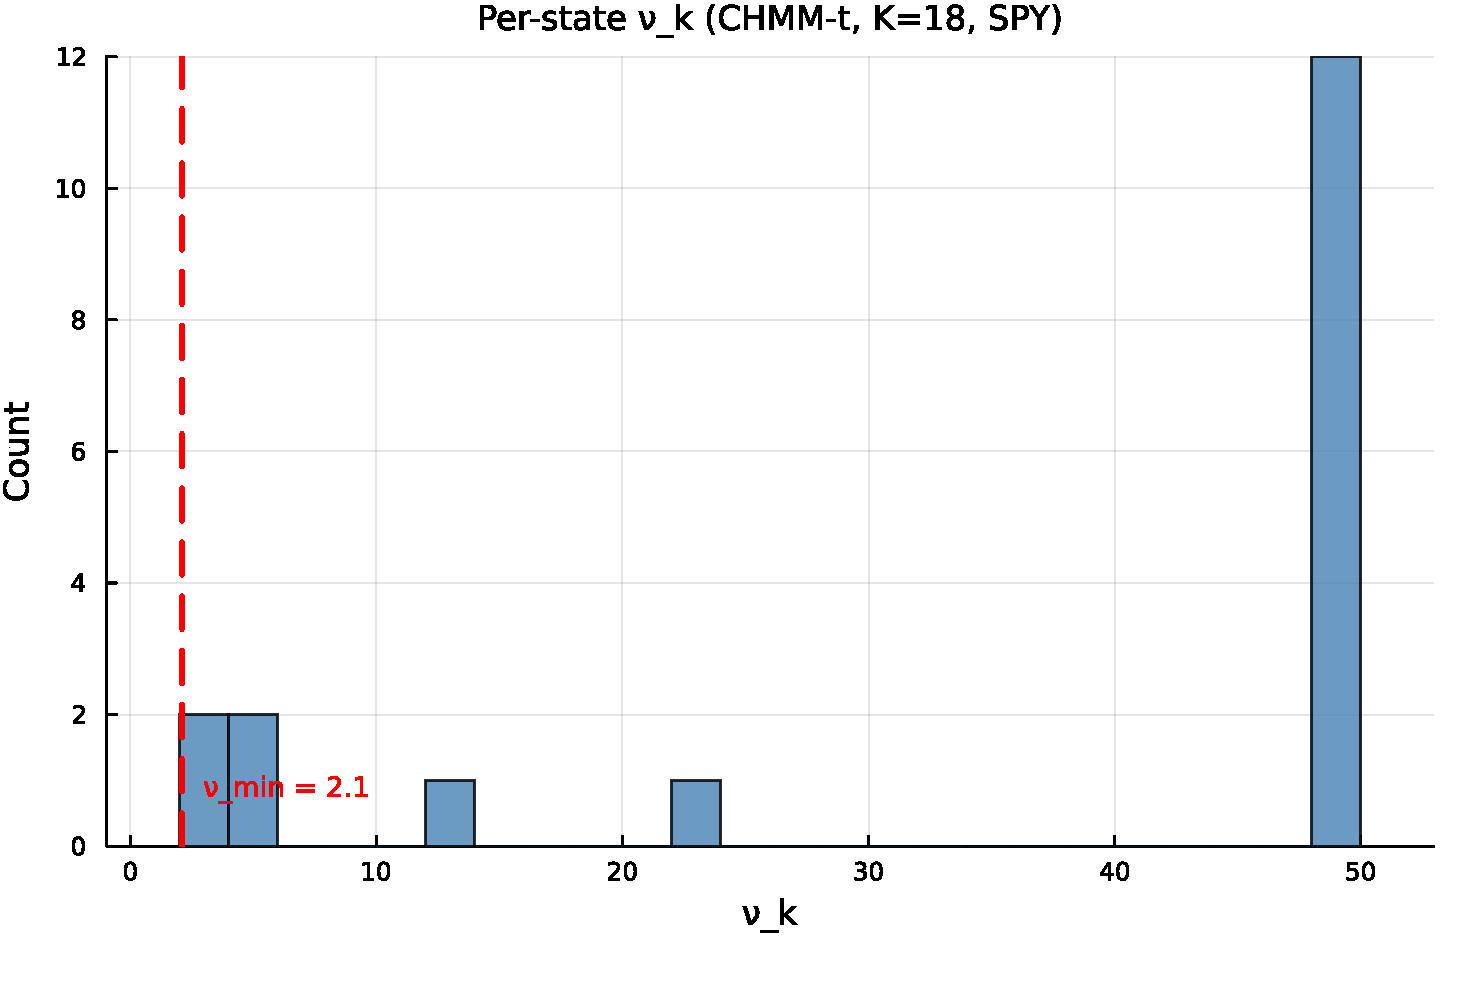
\includegraphics[width=0.65\textwidth]{figs/Fig-nu-Histogram.pdf}
\caption{Per-state degrees-of-freedom $\nu_k$ for the CHMM-t fit at $K = 18$ on SPY IS. The dashed red line marks the lower ECM bracket $\nu_{\min} = 2.1$. Only two states ($\nu_2 = 2.19$, $\nu_4 = 2.10$) sit near the lower bracket; the median $\nu_k$ is at the upper bracket.}
\label{fig:nu_hist}
\end{figure}

\paragraph{CHMM-GED per-state $p_k$ (Gaussian-bulk / Laplace-tail bimodality).}
The generator comparison reports and discusses the $\hat p_k$ partition (Figure~\ref{fig:p_hist}). Briefly, the $K = 18$ CHMM-GED fit on SPY IS was bimodal: eleven states attained exactly $p_k = 3.0$ (thirteen were Gaussian-like with $p_k \ge 1.85$), one state landed at intermediate $p_k = 1.6$, and four states clustered in the Laplace-shape regime $p_k \in [0.86, 1.24]$, concentrated in the high-volatility ranks. The smallest fitted $p_k$ on SPY was $0.86$, well clear of every $p_{\min}$ tested in the bracket sweep, so the lower bracket was non-binding. The bimodal partition replicated across $10$ Monte Carlo seeds and across the cross-asset universe (full robustness panel in the cross-asset robustness appendix).

\paragraph{Bracket-sensitivity sweeps.}
A CHMM-t bracket sweep on $\nu_{\min} \in \{2.1, 2.5, 3.0, 4.0, \infty\}$ at $K = 18$ showed that the excess kurtosis overshoot is a feature of the Student-$t$ emission at $K = 18$, not a lower-bracket artefact. The simulated IS excess kurtosis stayed in a heavy-tailed band across finite brackets and collapsed only in the full Gaussian limit. The analogous CHMM-GED sweep on $p_{\max} \in \{2.0, 2.5, 3.0, 3.5, 4.0\}$ left the non-Gaussian state count invariant, with Laplace-like states in $\{3,4,5\}$; tightening $p_{\max}$ from $4.0$ to $3.0$ cost only a few nats of LL. The $p_{\min}$ sweep on $\{0.5, 0.7, 0.85\}$ was fully degenerate: every floor produced an identical fit because the smallest observed $\hat p_k$ on SPY was $0.86$.


\paragraph{Evaluation summary.}
Observed growth rates $G_t$ are fit by Baum-Welch CHMM at the default $K^\star = 3$, with $K = 18$ retained as the sensitivity reference for excess kurtosis fidelity; $1{,}000$ paths are then simulated and per-asset metrics computed (Table~\ref{tab:model_comparison}). For the multi-asset analysis we reuse the per-asset $K^\star = 3$ fits as marginals, draw a copula sample $\mathbf U \sim \mathcal C(\Sigma)$ from the fitted Student-$t$ copula on ranks, rank-reorder the per-asset single-asset paths to match $\mathbf U$, and report cross-asset metrics (Table~\ref{tab:cross_asset}). The single-asset CHMM framework is shared across both; the CHMM training and simulation steps are Algorithms~\ref{alg:chmm_em} and~\ref{alg:chmm_simulate}, the cross-asset rank-reordering step is Algorithm~\ref{alg:copula_sim}, and the architecture diagram for the single-asset framework is Figure~\ref{fig:chmm_architecture}.


\subsection{Validation Metric Details}
\label{sec:supp_metrics}
\subsection{Validation Metric Details}
\label{sec:metric_details}

This appendix documents the precise form of the seven per-path metrics referenced in Section~\ref{sec:metrics}.
For each model, 1{,}000 independent paths of length $T$ are simulated (200 paths for the cross-asset extension) and each metric is computed per path before aggregation.

\paragraph{Kolmogorov--Smirnov (KS) pass rate.}
The two-sample KS statistic \cite{kolmogorov1933, smirnov1948} measures the maximum vertical distance between two empirical CDFs,
\begin{equation}
    D_{n,m} = \sup_x |F_n(x) - G_m(x)|.
    \label{eq:ks}
\end{equation}
The KS pass rate is the fraction of paths for which the test fails to reject distributional equivalence against the reference data at $\alpha = 0.05$.

\paragraph{Anderson--Darling (AD) pass rate.}
The AD test is the integrated squared CDF deviation with a quadratic tail weighting, making it more sensitive than KS to tail discrepancies.
The AD pass rate is the fraction of paths for which the two-sample AD test fails to reject at $\alpha = 0.05$.

\paragraph{Excess kurtosis.}
Mean simulated excess kurtosis across paths, compared to the observed value.
Given Gaussian emissions, the CHMM is expected to underestimate kurtosis relative to the heavy-tailed empirical distribution, and the shortfall is one of the reported diagnostics.

\paragraph{ACF-MAE.}
Mean absolute error between observed and mean-simulated autocorrelation functions of $|G_t|$ over $L = 252$ lags,
\begin{equation}
    \text{ACF-MAE} = \frac{1}{L}\sum_{\tau=1}^{L} \left| \hat\rho^{\text{obs}}_{|G|}(\tau) - \bar{\hat\rho}^{\,\text{sim}}_{|G|}(\tau) \right|.
    \label{eq:acf_mae_supp}
\end{equation}
This is the direct diagnostic for the Ryd\'{e}n et al.\ limitation.

\paragraph{Wasserstein-1 distance.}
The mean absolute difference of sorted empirical quantiles, equivalent to the $L^1$ distance between the empirical CDFs \cite{glasserman2003monte},
\begin{equation}
    W_1(F, G) = \int_0^1 |F^{-1}(u) - G^{-1}(u)|\, du.
    \label{eq:wasserstein}
\end{equation}

\paragraph{Hellinger distance.}
A histogram-based overlap distance in $[0, 1]$,
\begin{equation}
    H(P, Q) = \frac{1}{\sqrt{2}}\sqrt{\sum_{i=1}^{B}\left(\sqrt{p_i} - \sqrt{q_i}\right)^2},
    \label{eq:hellinger}
\end{equation}
with $B$ equal-width bins spanning the joint support and $p_i, q_i$ the observed and simulated bin probabilities.

\paragraph{Quantile coverage.}
The fraction of 99 equally-spaced observed quantiles (1st through 99th percentile) falling inside the 5th--95th percentile envelope of the corresponding simulated quantile across 1{,}000 paths.
A coverage of 100\% indicates that the simulation envelope fully brackets the observed distribution at every percentile.

\paragraph{Cross-asset metrics.}
For the cross-asset extension we additionally track the mean Frobenius norm $\|\hat\Sigma_{\text{sim}}^{(p)} - \hat\Sigma_{\text{obs}}\|_F$ and the off-diagonal Pearson correlation MAE between simulated and observed return matrices, averaged over paths.



\subsection{Formal Theoretical Statements}
\label{sec:supp_propositions}

The following propositions are referenced in Section~\ref{sec:theory} and stated formally here for reference; each is a one-line specialisation of a standard result and the proof sketch is one sentence.

\begin{proposition}[ECM monotonicity for CHMM-t (and EM monotonicity for CHMM-N, CHMM-L)]
\label{prop:ecm_monotone}
Under compactness of the parameter space ($\mu_k$, $\sigma_k$ or $b_k$, $\nu_k$ each in a closed bounded interval, $T_{ij} \ge \epsilon_T > 0$), the two-block CM step for CHMM-t of Section~\ref{sec:mstep}, namely the closed-form weighted updates of $(\mathbf T, \boldsymbol\pi, \mu_k, \sigma_k)$ at fixed $\nu_k$, followed by a golden-section maximisation of the per-state $Q$-function over $\nu_k \in [\nu_{\min}, \nu_{\max}]$, satisfies $Q(\theta^{(n+1)} \mid \theta^{(n)}) \ge Q(\theta^{(n)} \mid \theta^{(n)})$, and consequently $\mathcal L(\theta^{(n+1)}) \ge \mathcal L(\theta^{(n)})$ where $\mathcal L$ is the incomplete-data log-likelihood. The same monotonicity holds for the closed-form CHMM-N and CHMM-L M-steps under the standard EM guarantee.
\end{proposition}
\noindent\emph{Proof sketch.} Each CM step does not decrease $Q$ by definition (CM-1 is closed-form maximum, CM-2 is golden-section maximum); the standard EM inequality $\mathcal L(\theta^{(n+1)}) - \mathcal L(\theta^{(n)}) \ge Q(\theta^{(n+1)} \mid \theta^{(n)}) - Q(\theta^{(n)} \mid \theta^{(n)})$ \cite{wu1983convergence, mengrubin1993ecm} converts $Q$-monotonicity into log-likelihood monotonicity. Compactness gives boundedness above, hence convergence.

\begin{proposition}[Identifiability up to label permutation]
\label{prop:identifiability}
Under irreducibility and aperiodicity of $\mathbf T$ (Assumption~\ref{ass:irred}) and the emission contrast condition (Assumption~\ref{ass:moments}), the CHMM parameter is identifiable up to label permutation in all three emission families considered (CHMM-N, CHMM-t with $\nu_k \in [\nu_{\min}, \nu_{\max}]$, and CHMM-L).
\end{proposition}
\noindent\emph{Proof sketch.} The HMM identifiability theorem of \citet{allman2009identifiability} requires $\mathbf T$ of full rank and per-state emissions linearly independent in the space of densities on $\R$. Full-rank $\mathbf T$ follows from irreducibility \cite{levinperes2017markov}; linear independence of Gaussian, bracketed-$\nu$ Student-t, and Laplace emissions with distinct location-scale parameters follows from \citet{yakowitzspragins1968}.

\begin{proposition}[MLE consistency]
\label{prop:consistency}
Under Assumptions~\ref{ass:irred}--\ref{ass:moments} and the assumption that the true parameter lies in the interior of a compact $\Theta$, the MLE $\hat\theta_T = \arg\max_{\theta \in \Theta} \mathcal L_T(\theta)$ is consistent: $\hat\theta_T \xrightarrow{p} \theta_0$ as $T \to \infty$, modulo label permutation.
\end{proposition}
\noindent\emph{Proof reference.} \citet{bickel1998asymptotic} (Theorem~1) and \citet{doucmoulinesryden2004} apply directly under our assumption set: irreducibility supplies the mixing condition, finite second moment the moment condition, compactness the parameter-space condition.

\begin{proposition}[Marginal preservation under rank reordering]
\label{prop:rank_marginals}
Let $\tilde g_{j, 1:T}$ be a sample of size $T$ from the per-asset CHMM marginal of asset $j$, and let the rank-reordered output be $\hat g_{j,t}^{(p)} = \tilde g_{j, (r_{j,t}^{(p)})}^{(p)}$ where $r_{j,t}^{(p)}$ is the rank of the copula sample. Then for every asset $j$ the empirical CDF of $\{\hat g_{j,t}^{(p)}\}_{t=1}^T$ equals that of $\{\tilde g_{j,t}^{(p)}\}_{t=1}^T$.
\end{proposition}
\noindent\emph{Proof sketch.} The map $t \mapsto r_{j,t}^{(p)}$ is a permutation almost surely, so the multiset of values is preserved; the empirical CDF depends only on the multiset.

\subsection{State-Resolution and Multi-Emission Sensitivity}
\label{sec:supp_sensitivity}
\subsubsection{Full State-Resolution Sensitivity Table}
\label{sec:sensitivity_table}

Table~\ref{tab:sensitivity} reports the full $K$-sweep referenced in Section~\ref{sec:k_selection_results} of the main text.
Observed excess kurtosis is $7.68$ IS and $5.29$ OoS at all $K$.

\begin{table}[H]
\centering
\caption{State resolution sensitivity for SPY CHMM-N (1{,}000 paths, $\alpha = 0.05$). Every metric is computed on the identical simulation pipeline used for Table~\ref{tab:model_comparison} in the main text. IS coverage was 100\% at every $K$; OoS coverage is reported separately. ACF-MAE columns: $|G_t|$ measures the volatility-clustering reproduction; $G_t$ measures linear-autocorrelation reproduction (parallel to $|G_t|$, both averaged over lags 1--252).}
\label{tab:sensitivity}
\small
\begin{tabular}{c cc cc cc cc c c c}
\toprule
& \multicolumn{2}{c}{KS (\%)} & \multicolumn{2}{c}{AD (\%)} & \multicolumn{2}{c}{Kurtosis} & \multicolumn{2}{c}{ACF-MAE} & & & \\
\cmidrule(lr){2-3} \cmidrule(lr){4-5} \cmidrule(lr){6-7} \cmidrule(lr){8-9}
$K$ & IS & OoS & IS & OoS & Obs & Sim & $|G_t|$ & $G_t$ & $W_1$ & $H$ & Cov OoS (\%) \\
\midrule
3  & 89.0 & 77.2 & 78.9 & 68.6 & 7.68 & 3.82 & 0.0463 & 0.0240 & 0.131 & 0.0839 & 94.9 \\
6  & 92.9 & 78.7 & 84.3 & 74.3 & 7.68 & 5.38 & 0.0496 & 0.0238 & 0.116 & 0.0829 & 90.9 \\
9  & 93.0 & 81.4 & 84.4 & 74.4 & 7.68 & 4.63 & 0.0492 & 0.0238 & 0.118 & 0.0810 & 91.9 \\
12 & 94.9 & 81.6 & 85.8 & 75.0 & 7.68 & 4.57 & 0.0500 & 0.0238 & 0.113 & 0.0801 & 91.9 \\
15 & 93.9 & 81.0 & 84.8 & 73.5 & 7.68 & 4.89 & 0.0508 & 0.0238 & 0.114 & 0.0804 & 88.9 \\
\textbf{18} & 94.8 & 85.5 & 88.2 & 79.7 & 7.68 & 5.04 & 0.0515 & 0.0237 & 0.110 & 0.0807 & 91.9 \\
21 & \textbf{95.6} & \textbf{88.0} & \textbf{89.1} & \textbf{78.8} & 7.68 & 3.78 & 0.0534 & \textbf{0.0236} & 0.112 & 0.0801 & \textbf{99.0} \\
\bottomrule
\end{tabular}
\end{table}

\subsubsection{Multi-Emission State-Resolution Sensitivity}
\label{sec:multi_emission_sensitivity}

Table~\ref{tab:sensitivity_multi} extends Table~\ref{tab:sensitivity} across the three emission families, confirming that the qualitative operating point $K = 18$ is stable when the Gaussian component is replaced with Student-t or Laplace emissions.
For CHMM-t the per-state degrees of freedom $\nu_k$ are refit by ECM-plus-golden-section at every $K$; for CHMM-L the weighted-median location and weighted MAD scale are closed form and impose no additional cost.
Three patterns extend from Table~\ref{tab:sensitivity} to the new families.
First, the distributional pass rates plateau in the $K \in \{12, 15, 18, 21\}$ band for all three families: CHMM-t reaches its highest IS KS at $K = 18$ ($96.0\%$) and its highest OoS KS at $K = 18$ ($84.5\%$), and CHMM-L reaches its highest IS KS at $K = 18$ ($95.6\%$) and its highest IS AD at $K = 18$ ($92.7\%$).
Once a family enters the plateau the operating point is flat with respect to $K$, so we report the main-text results at the same $K = 18$ used for CHMM-N.
Second, the absolute-return ACF-MAE remains within the narrow $0.047$--$0.056$ band observed for the Gaussian sweep, and the raw-return ACF-MAE remains essentially constant at $\approx 0.024$ across all $21$ (family, $K$) combinations. Both temporal axes are properties of the regime structure rather than the emission family: $|G_t|$ ACF reproduction is governed by the eigenvalue spectrum of $\mathbf T$ (Section~\ref{sec:theory}), and raw-$G_t$ ACF is null in expectation under any HMM with i.i.d.\ within-state emissions.
Third, simulated kurtosis behaves as expected from the component families: the Gaussian sweep peaks around $5.0$ at the high-$K$ end, the Laplace sweep lands squarely in the $5.3$--$6.7$ range (closest to the observed $7.68$), and the Student-t sweep climbs sharply above $13$ across the entire sweep because the ECM search assigns small $\nu_k$ to a subset of tail states, over-correcting IS kurtosis.

\begin{table}[H]
\centering
\caption{Multi-emission state resolution sensitivity for SPY (1{,}000 paths, $\alpha = 0.05$). CHMM-N: Gaussian; CHMM-t: Student-t with per-state $\nu_k$ refit by ECM-plus-golden-section; CHMM-L: Laplace with weighted-median location and weighted-MAD scale. Every metric is computed on the identical simulation pipeline used for Table~\ref{tab:model_comparison}. Observed excess kurtosis is $7.68$ IS and $5.29$ OoS. ACF-MAE columns parallel the main-text Table~\ref{tab:model_comparison}: $|G_t|$ for volatility clustering, $G_t$ (raw) for linear autocorrelation.}
\label{tab:sensitivity_multi}
\small
\resizebox{\textwidth}{!}{%
\begin{tabular}{l c cc cc c cc c c}
\toprule
& & \multicolumn{2}{c}{KS (\%)} & \multicolumn{2}{c}{AD (\%)} & & \multicolumn{2}{c}{ACF-MAE} & & \\
\cmidrule(lr){3-4} \cmidrule(lr){5-6} \cmidrule(lr){8-9}
Family & $K$ & IS & OoS & IS & OoS & Kurt (IS sim) & $|G_t|$ & $G_t$ & $W_1$ IS & $H$ IS \\
\midrule
CHMM-N & 3  & 89.7 & 80.1 & 79.2 & 70.7 & 3.86  & 0.0467 & 0.0240 & 0.128 & 0.0833 \\
       & 6  & 93.8 & 79.1 & 87.2 & 72.8 & 5.29  & 0.0504 & 0.0238 & 0.114 & 0.0825 \\
       & 9  & 94.9 & 83.0 & 84.3 & 74.8 & 4.58  & 0.0490 & 0.0238 & 0.115 & 0.0806 \\
       & 12 & 93.7 & 82.7 & 85.5 & 75.0 & 4.56  & 0.0501 & 0.0237 & 0.115 & 0.0804 \\
       & 15 & 93.6 & 83.0 & 87.0 & 75.1 & 4.89  & 0.0509 & 0.0238 & 0.114 & 0.0803 \\
       & \textbf{18} & 94.7 & 83.4 & 88.5 & 76.6 & 4.97  & 0.0511 & 0.0237 & 0.108 & 0.0805 \\
       & 21 & \textbf{95.1} & \textbf{88.0} & \textbf{88.2} & \textbf{79.7} & 3.80  & 0.0532 & 0.0236 & 0.110 & 0.0796 \\
\midrule
CHMM-t & 3  & 92.2 & 82.9 & 88.0 & 79.1 & 33.68 & 0.0538 & 0.0235 & 0.108 & 0.0759 \\
       & 6  & 91.8 & 80.4 & 86.7 & 74.8 & 22.74 & 0.0527 & 0.0235 & 0.108 & 0.0772 \\
       & 9  & 95.4 & 84.0 & 89.9 & 78.0 & 16.60 & 0.0535 & 0.0234 & 0.102 & 0.0752 \\
       & 12 & 95.2 & 85.0 & 89.8 & 78.4 & 14.98 & 0.0543 & 0.0234 & 0.100 & 0.0757 \\
       & 15 & 94.7 & 83.7 & 88.8 & 79.5 & 16.36 & 0.0539 & 0.0234 & 0.101 & 0.0758 \\
       & \textbf{18} & \textbf{96.0} & \textbf{84.5} & \textbf{91.7} & \textbf{80.8} & 13.19 & 0.0551 & \textbf{0.0234} & \textbf{0.099} & \textbf{0.0759} \\
       & 21 & 94.5 & 83.3 & 88.5 & 78.1 & 14.66 & 0.0539 & 0.0234 & 0.102 & 0.0758 \\
\midrule
CHMM-L & 3  & 81.9 & 64.8 & 82.5 & 65.8 & 5.29  & 0.0535 & 0.0235 & 0.112 & 0.0854 \\
       & 6  & 90.5 & 76.4 & 85.0 & 74.2 & 5.91  & 0.0513 & 0.0235 & 0.110 & 0.0818 \\
       & 9  & 90.5 & 75.7 & 84.8 & 70.1 & 6.01  & 0.0517 & 0.0235 & 0.110 & 0.0819 \\
       & 12 & 93.6 & 81.4 & 89.8 & 78.8 & 6.18  & 0.0541 & 0.0234 & 0.106 & 0.0796 \\
       & 15 & 92.5 & 78.9 & 88.3 & 78.8 & 6.03  & 0.0541 & 0.0234 & 0.105 & 0.0792 \\
       & \textbf{18} & \textbf{95.6} & \textbf{79.9} & \textbf{92.7} & \textbf{80.7} & \textbf{6.74}  & 0.0563 & 0.0234 & 0.101 & 0.0798 \\
       & 21 & 93.1 & 79.5 & 87.7 & 76.8 & 6.05  & 0.0543 & 0.0234 & 0.107 & 0.0807 \\
\bottomrule
\end{tabular}%
}
\end{table}

\subsubsection{Baum-Welch Convergence}
\label{sec:convergence}

Figure~\ref{fig:convergence_all} shows the Baum-Welch convergence curves for representative state resolutions.
All models converged within the 60-iteration budget, with the log-likelihood monotonically increasing (as guaranteed by the EM algorithm).
Lower $K$ values typically converged faster (15--25 iterations), while higher $K$ values required 25--40 iterations to reach the convergence tolerance of $|\Delta\mathcal{L}| < 10^{-4}$.
The monotonic increase confirms that the quantile-based initialization provided a valid starting point from which the EM algorithm could improve without encountering degenerate solutions.

\begin{figure}[H]
\centering
\begin{subfigure}[b]{0.32\textwidth}
    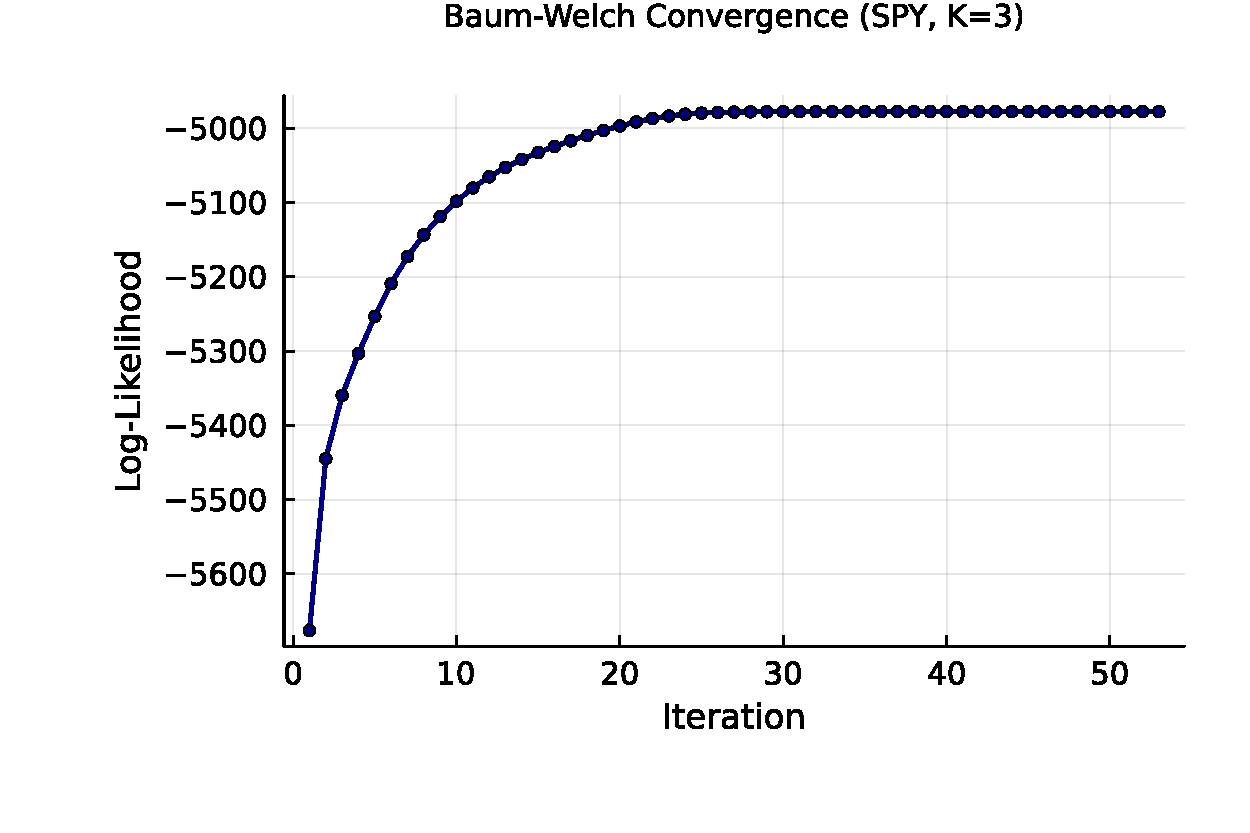
\includegraphics[width=\textwidth]{figs/Fig-Convergence-K3.pdf}
    \caption{$K = 3$}
\end{subfigure}
\hfill
\begin{subfigure}[b]{0.32\textwidth}
    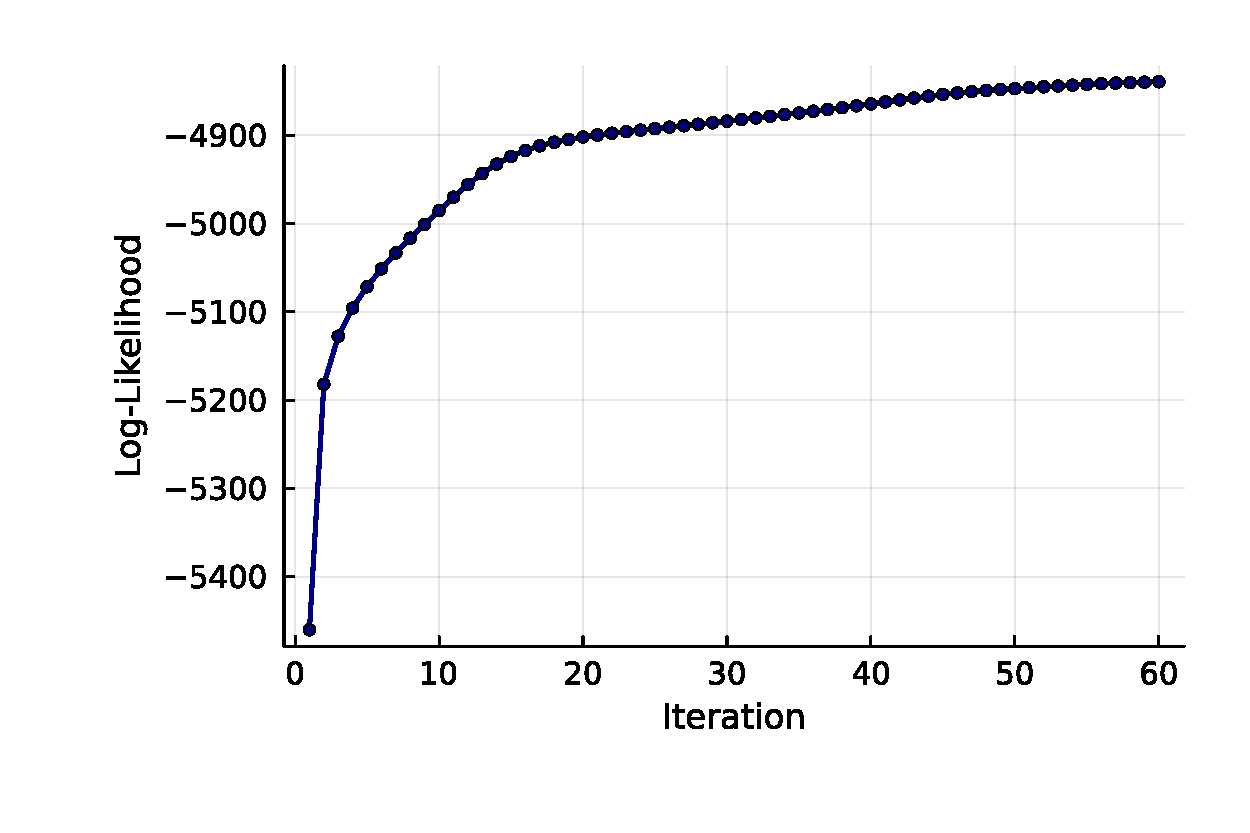
\includegraphics[width=\textwidth]{figs/Fig-Convergence-K12.pdf}
    \caption{$K = 12$}
\end{subfigure}
\hfill
\begin{subfigure}[b]{0.32\textwidth}
    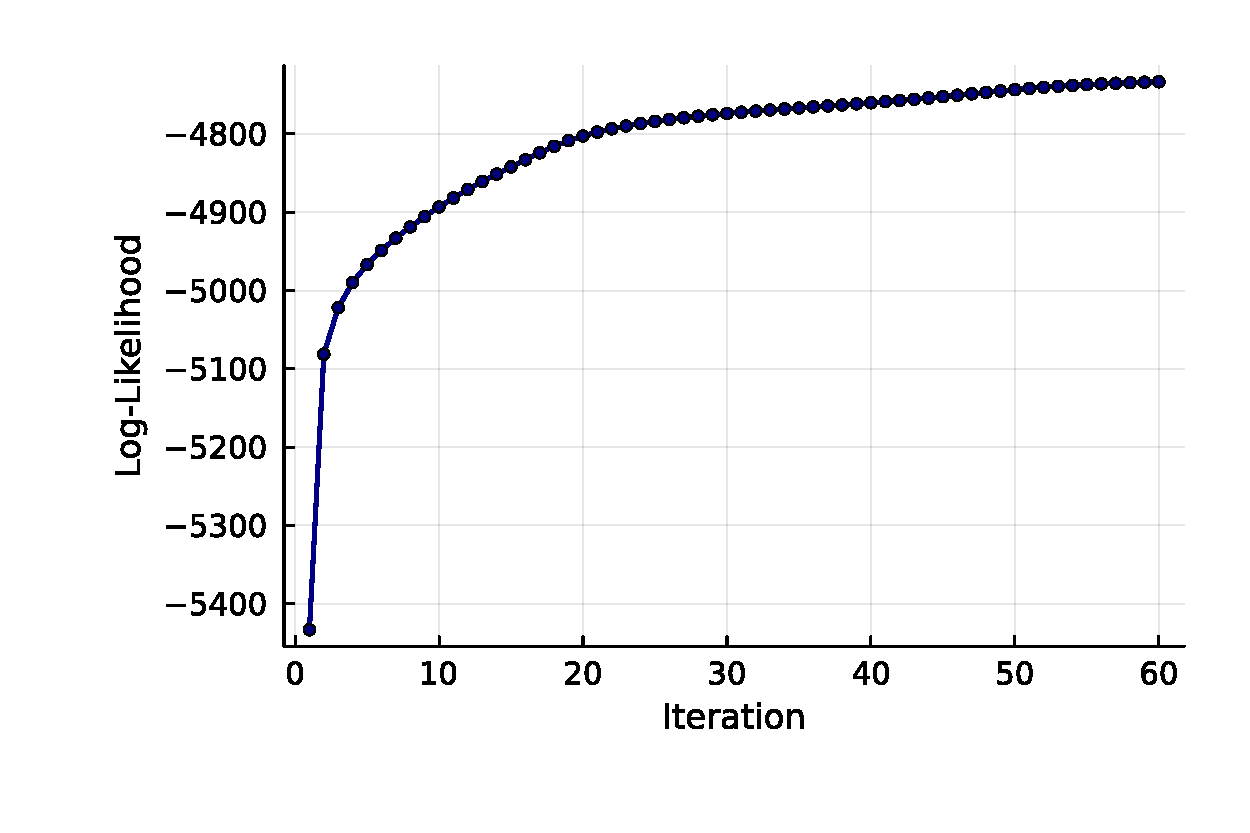
\includegraphics[width=\textwidth]{figs/Fig-Convergence-K18.pdf}
    \caption{$K = 18$ (selected)}
\end{subfigure}
\caption{Baum-Welch convergence for the SPY CHMM-N fit (Pipeline~A, IS) at selected state resolutions. Log-likelihood is monotonically increasing (EM guarantee) and plateaus well before $\texttt{max\_iter} = 60$.}
\label{fig:convergence_all}
\end{figure}

\subsubsection{IS Comparison at Non-Selected State Resolutions}
\label{sec:k_sweep_panels}

Figures~\ref{fig:k_sweep_panels_is}--\ref{fig:k_sweep_is_k21} show the IS model comparison panels for $K \in \{3, 6, 12, 21\}$, complementing the $K = 18$ comparison in Figure~\ref{fig:is_comparison} of the main text.
Across all resolutions, the CHMM's simulated density closely overlays the observed density, and the ACF of absolute returns tracks the slow decay pattern.
The visible improvement from $K = 3$ to $K = 18$ is concentrated in the tails of the Q-Q panel and the steady-state level of the ACF panel.
$K = 9$ and $K = 15$ panels are omitted because they interpolate smoothly between the shown resolutions; their numerical metrics are in Table~\ref{tab:sensitivity}.

\begin{figure}[H]
\centering
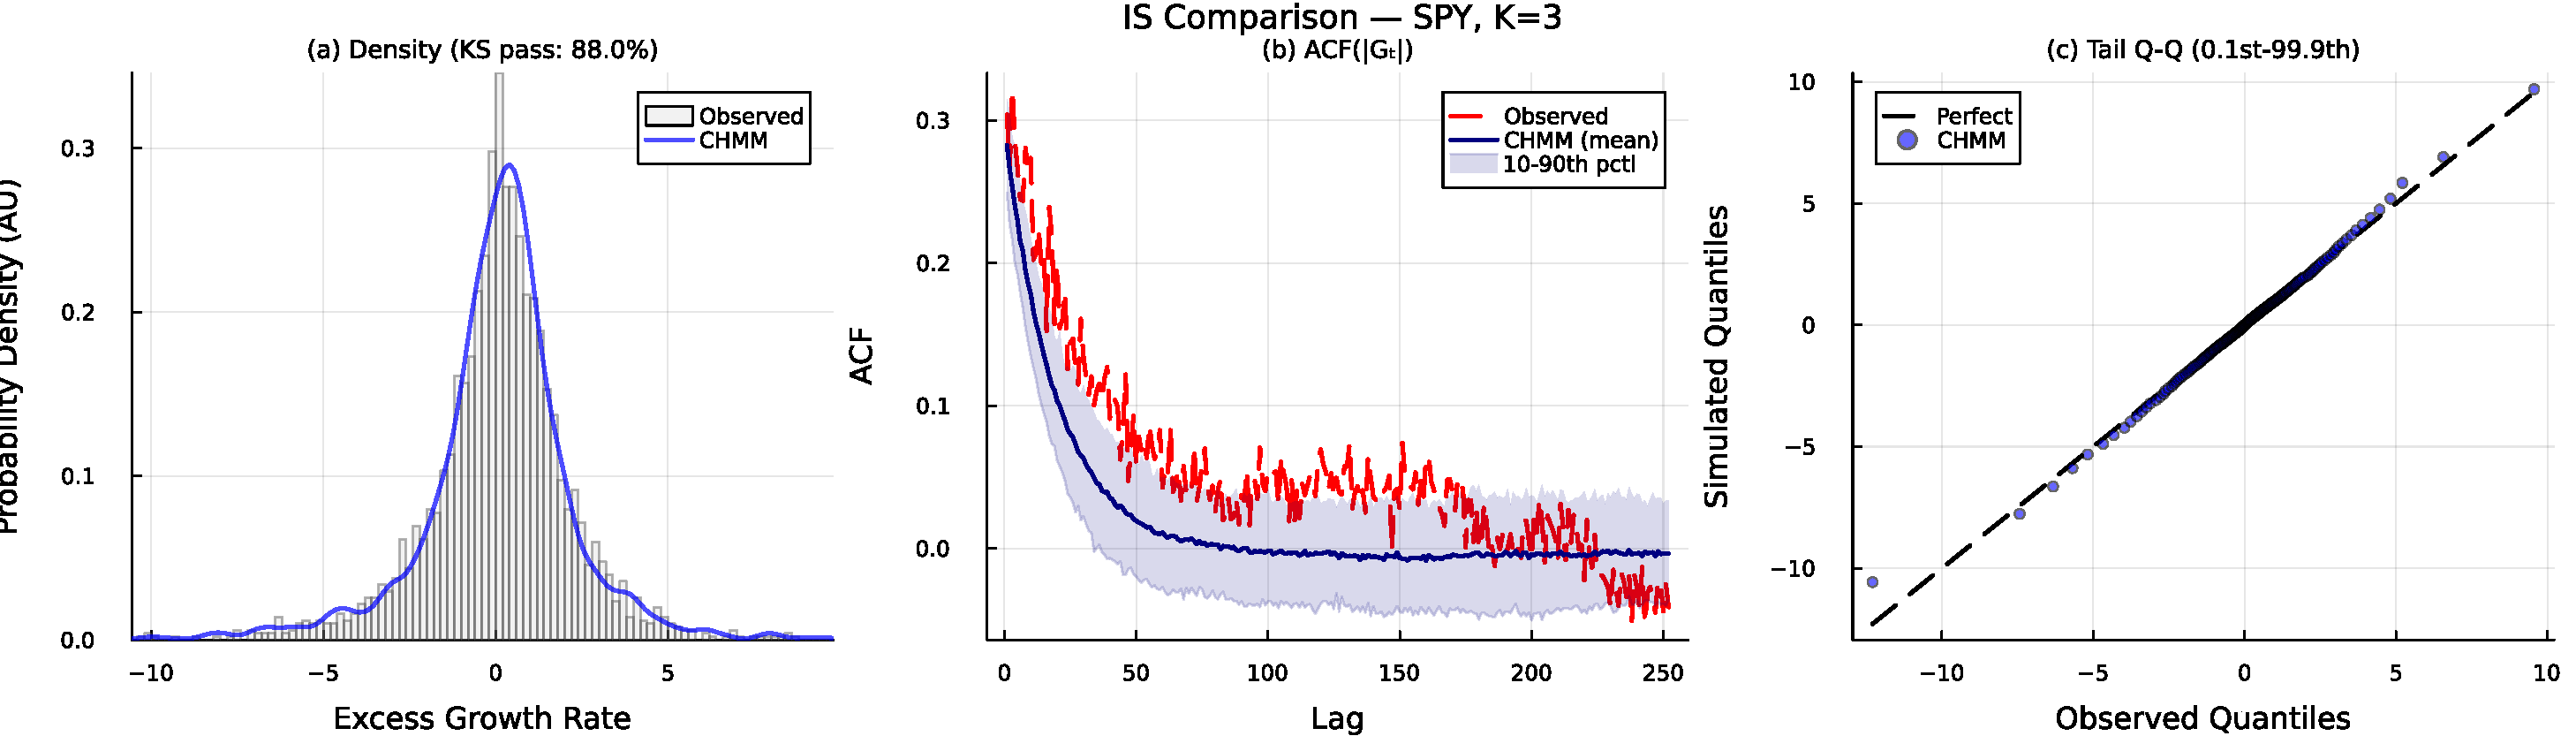
\includegraphics[width=\textwidth]{figs/Fig-3-IS-Comparison-K3.pdf}
\caption{IS SPY CHMM-N comparison at $K = 3$ (Pipeline~A, 1{,}000 simulated paths; panels as in Figure~\ref{fig:is_comparison}). The $K = 18$ counterpart is Figure~\ref{fig:is_comparison} of the main text.}
\label{fig:k_sweep_panels_is}
\end{figure}

\begin{figure}[H]
\centering
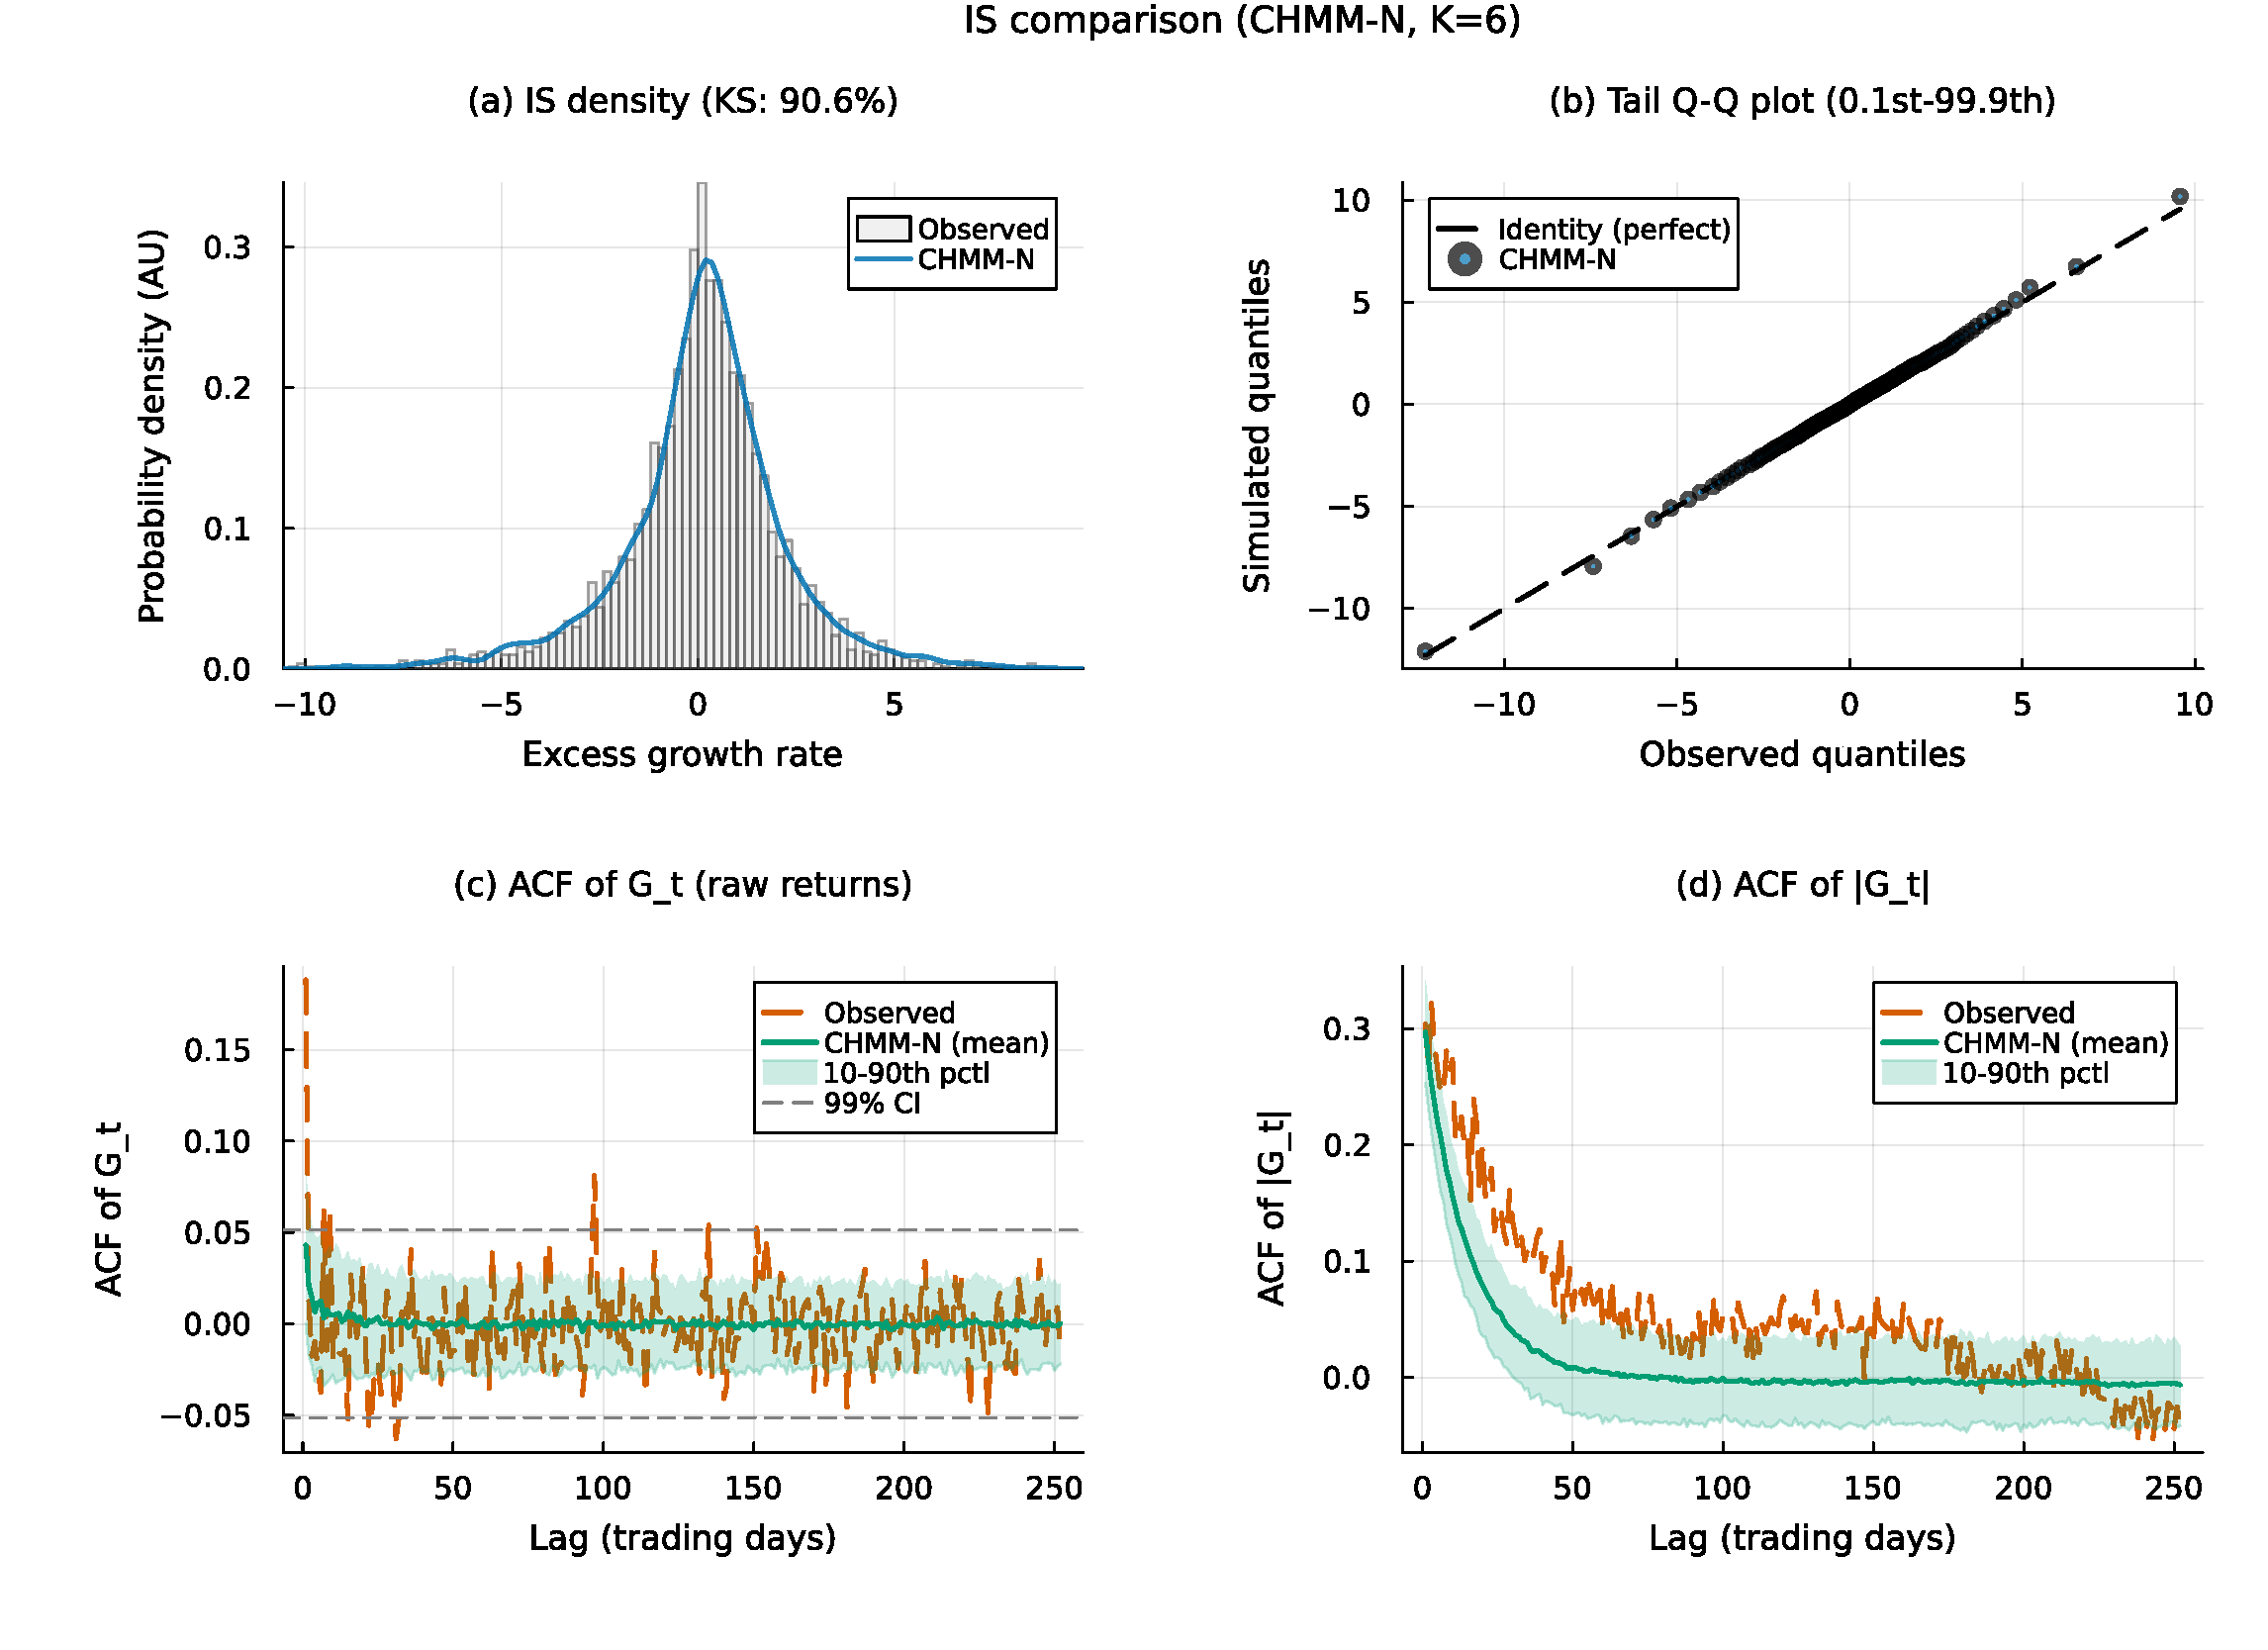
\includegraphics[width=\textwidth]{figs/Fig-3-IS-Comparison-K6.pdf}
\caption{IS SPY CHMM-N comparison at $K = 6$ (Pipeline~A, 1{,}000 simulated paths; panels as in Figure~\ref{fig:is_comparison}).}
\label{fig:k_sweep_is_k6}
\end{figure}

\begin{figure}[H]
\centering
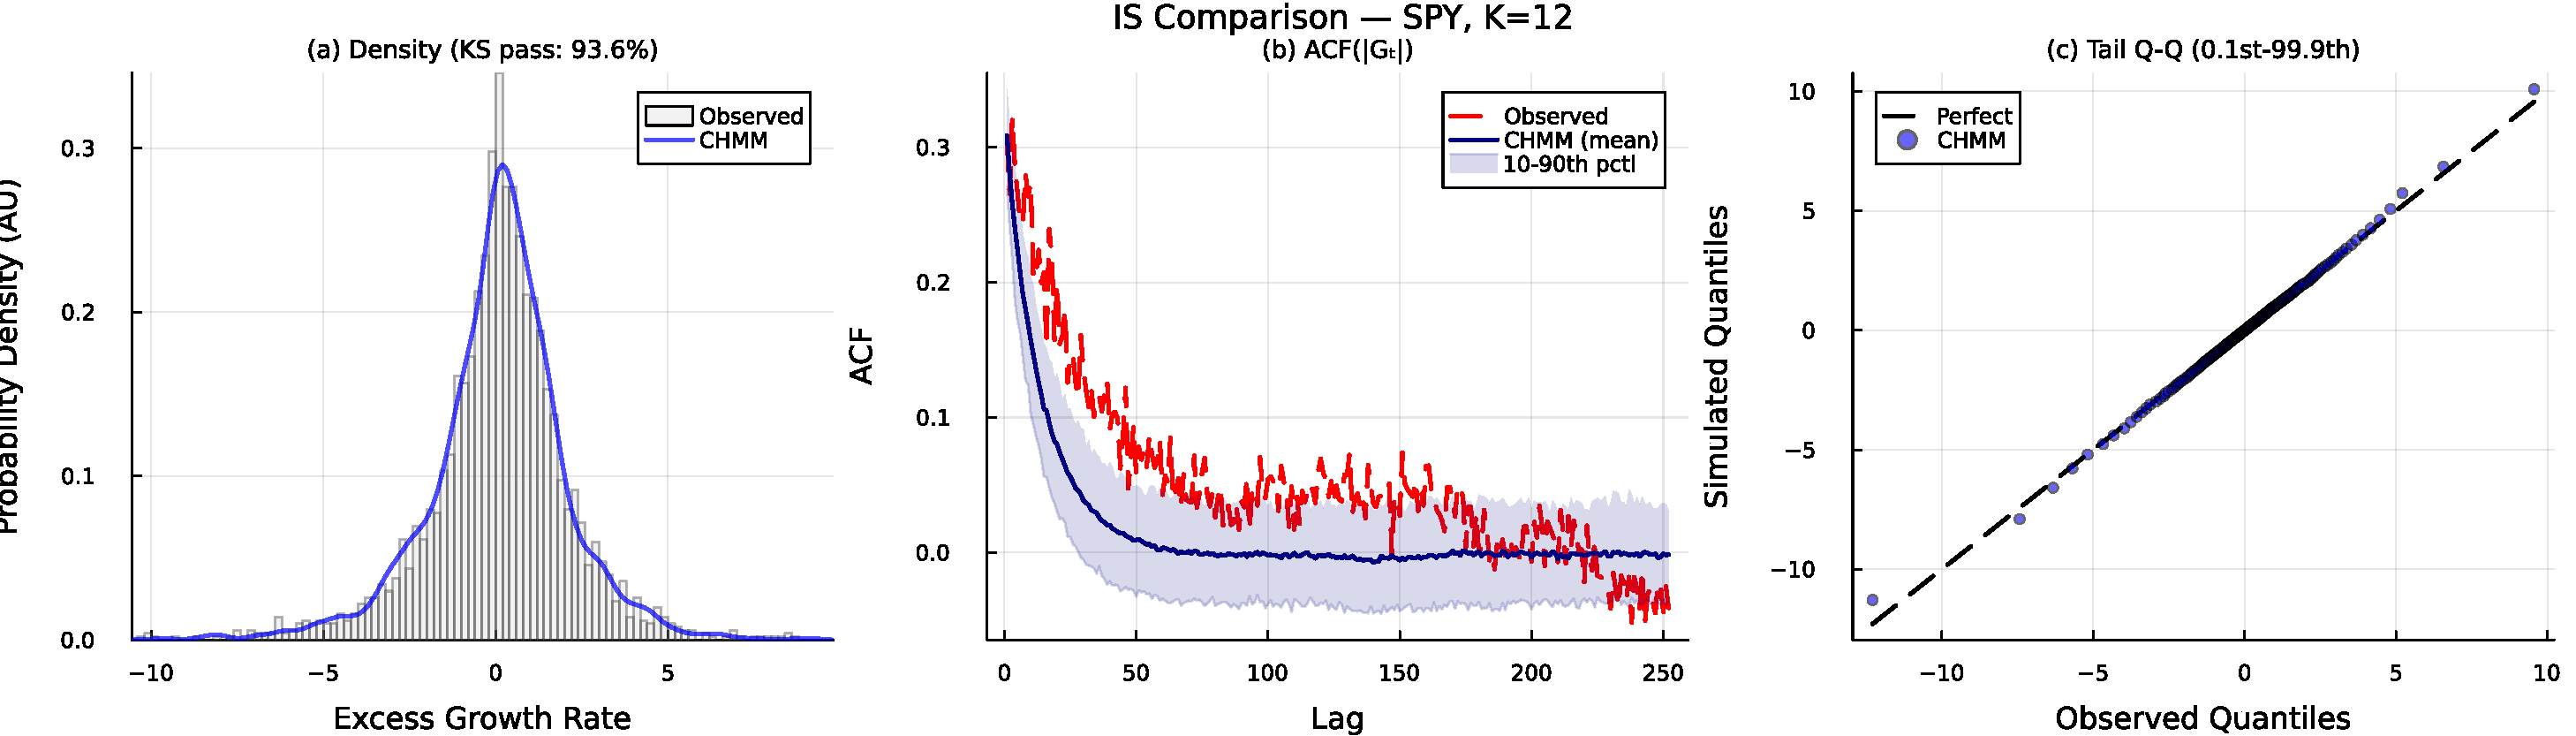
\includegraphics[width=\textwidth]{figs/Fig-3-IS-Comparison-K12.pdf}
\caption{IS SPY CHMM-N comparison at $K = 12$ (Pipeline~A, 1{,}000 simulated paths; panels as in Figure~\ref{fig:is_comparison}).}
\label{fig:k_sweep_is_k12}
\end{figure}

\begin{figure}[H]
\centering
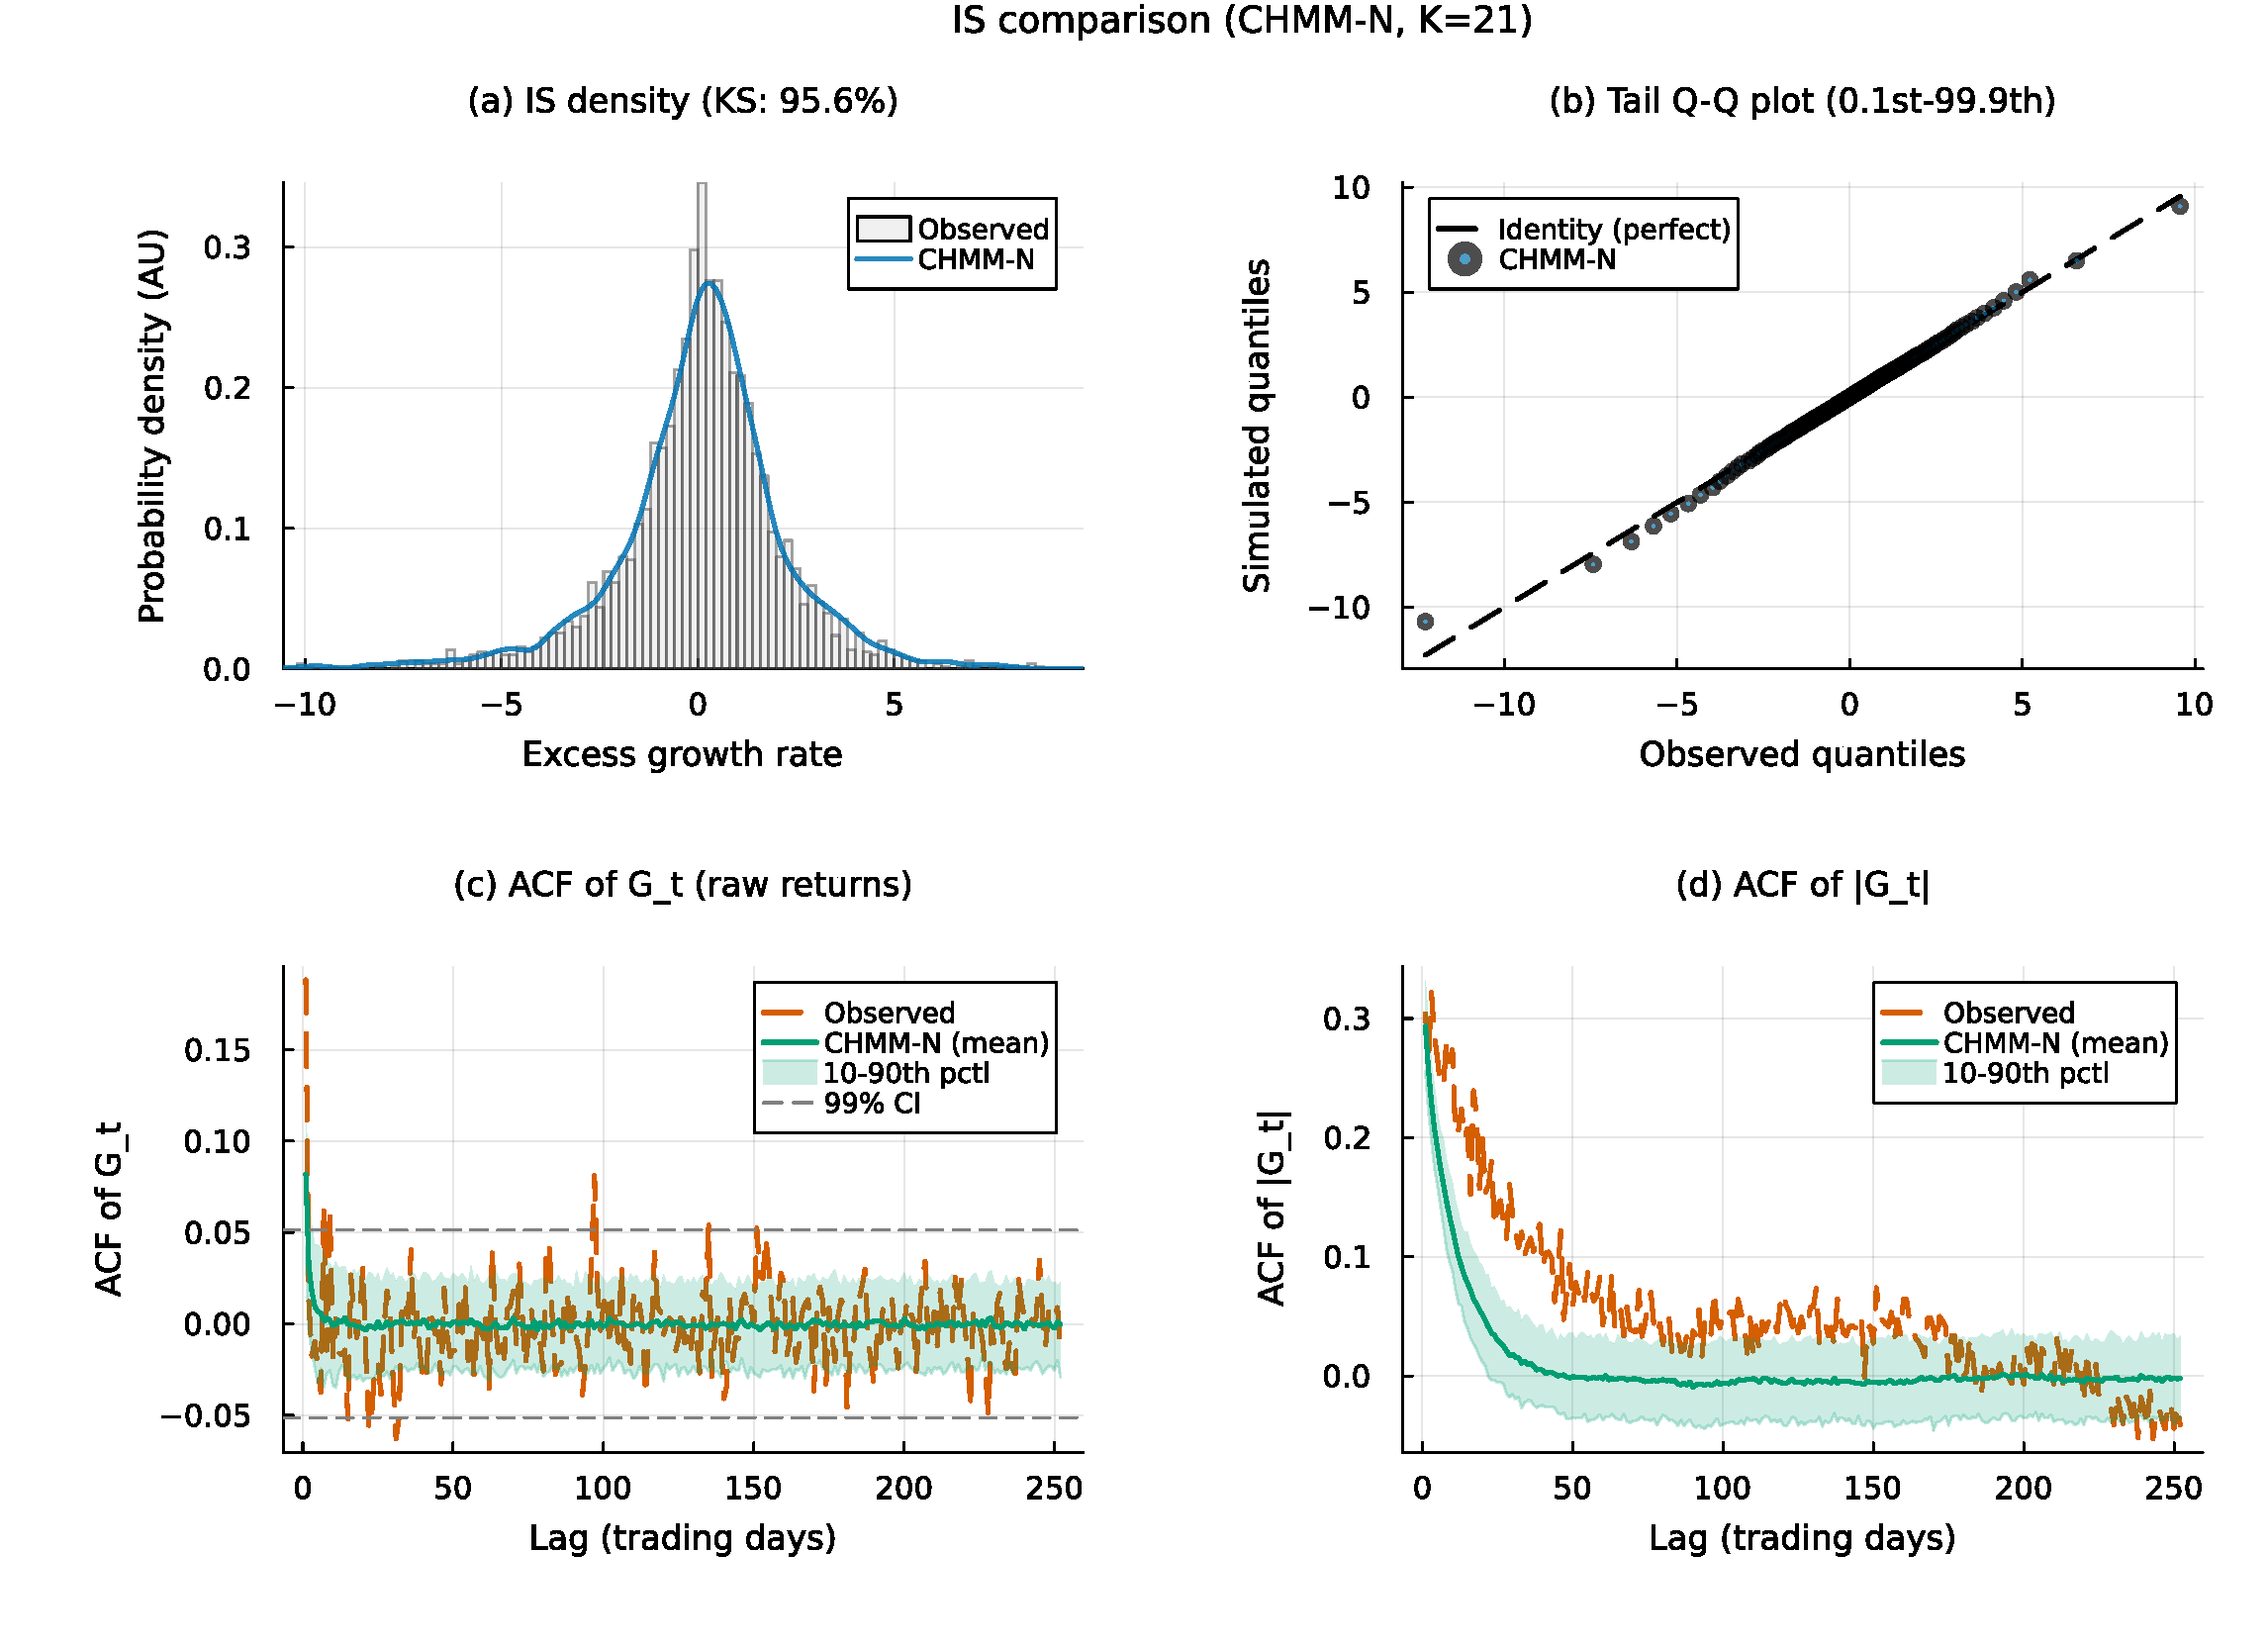
\includegraphics[width=\textwidth]{figs/Fig-3-IS-Comparison-K21.pdf}
\caption{IS SPY CHMM-N comparison at $K = 21$ (Pipeline~A, 1{,}000 simulated paths; panels as in Figure~\ref{fig:is_comparison}).}
\label{fig:k_sweep_is_k21}
\end{figure}

\subsubsection{OoS Validation at Non-Selected State Resolutions}

Figures~\ref{fig:k_sweep_panels_oos}--\ref{fig:k_sweep_oos_k21} show the OoS validation panels for $K \in \{3, 6, 12, 21\}$.
KS pass rates remain above 91\% at all resolutions; the $K = 18$ panel is reproduced in Figure~\ref{fig:oos_validation} of the main text.
As with the IS panels, $K = 9$ and $K = 15$ are omitted; numerical OoS KS pass rates are in Table~\ref{tab:sensitivity}.

\begin{figure}[H]
\centering
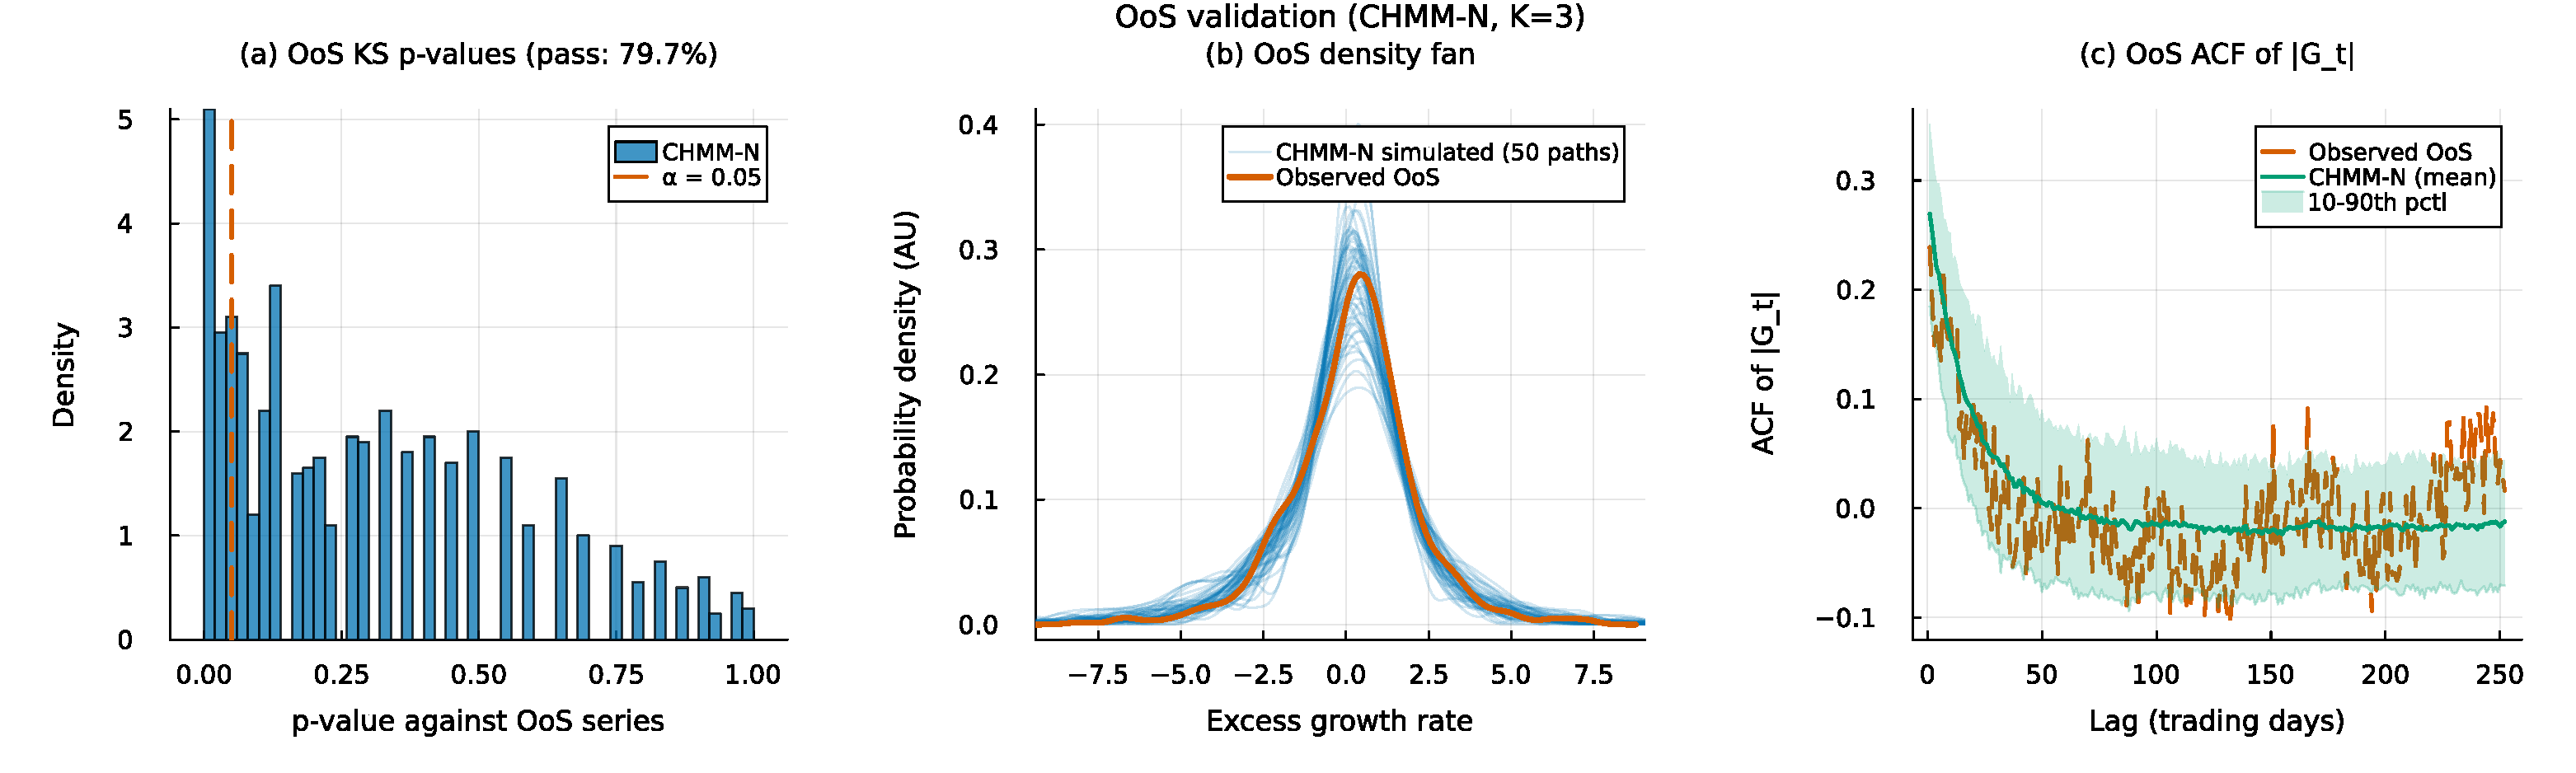
\includegraphics[width=\textwidth]{figs/Fig-4-OoS-Validation-K3.pdf}
\caption{OoS SPY CHMM-N validation at $K = 3$ (Pipeline~A, 1{,}000 simulated paths; panels as in Figure~\ref{fig:oos_validation}). The $K = 18$ counterpart is Figure~\ref{fig:oos_validation} of the main text.}
\label{fig:k_sweep_panels_oos}
\end{figure}

\begin{figure}[H]
\centering
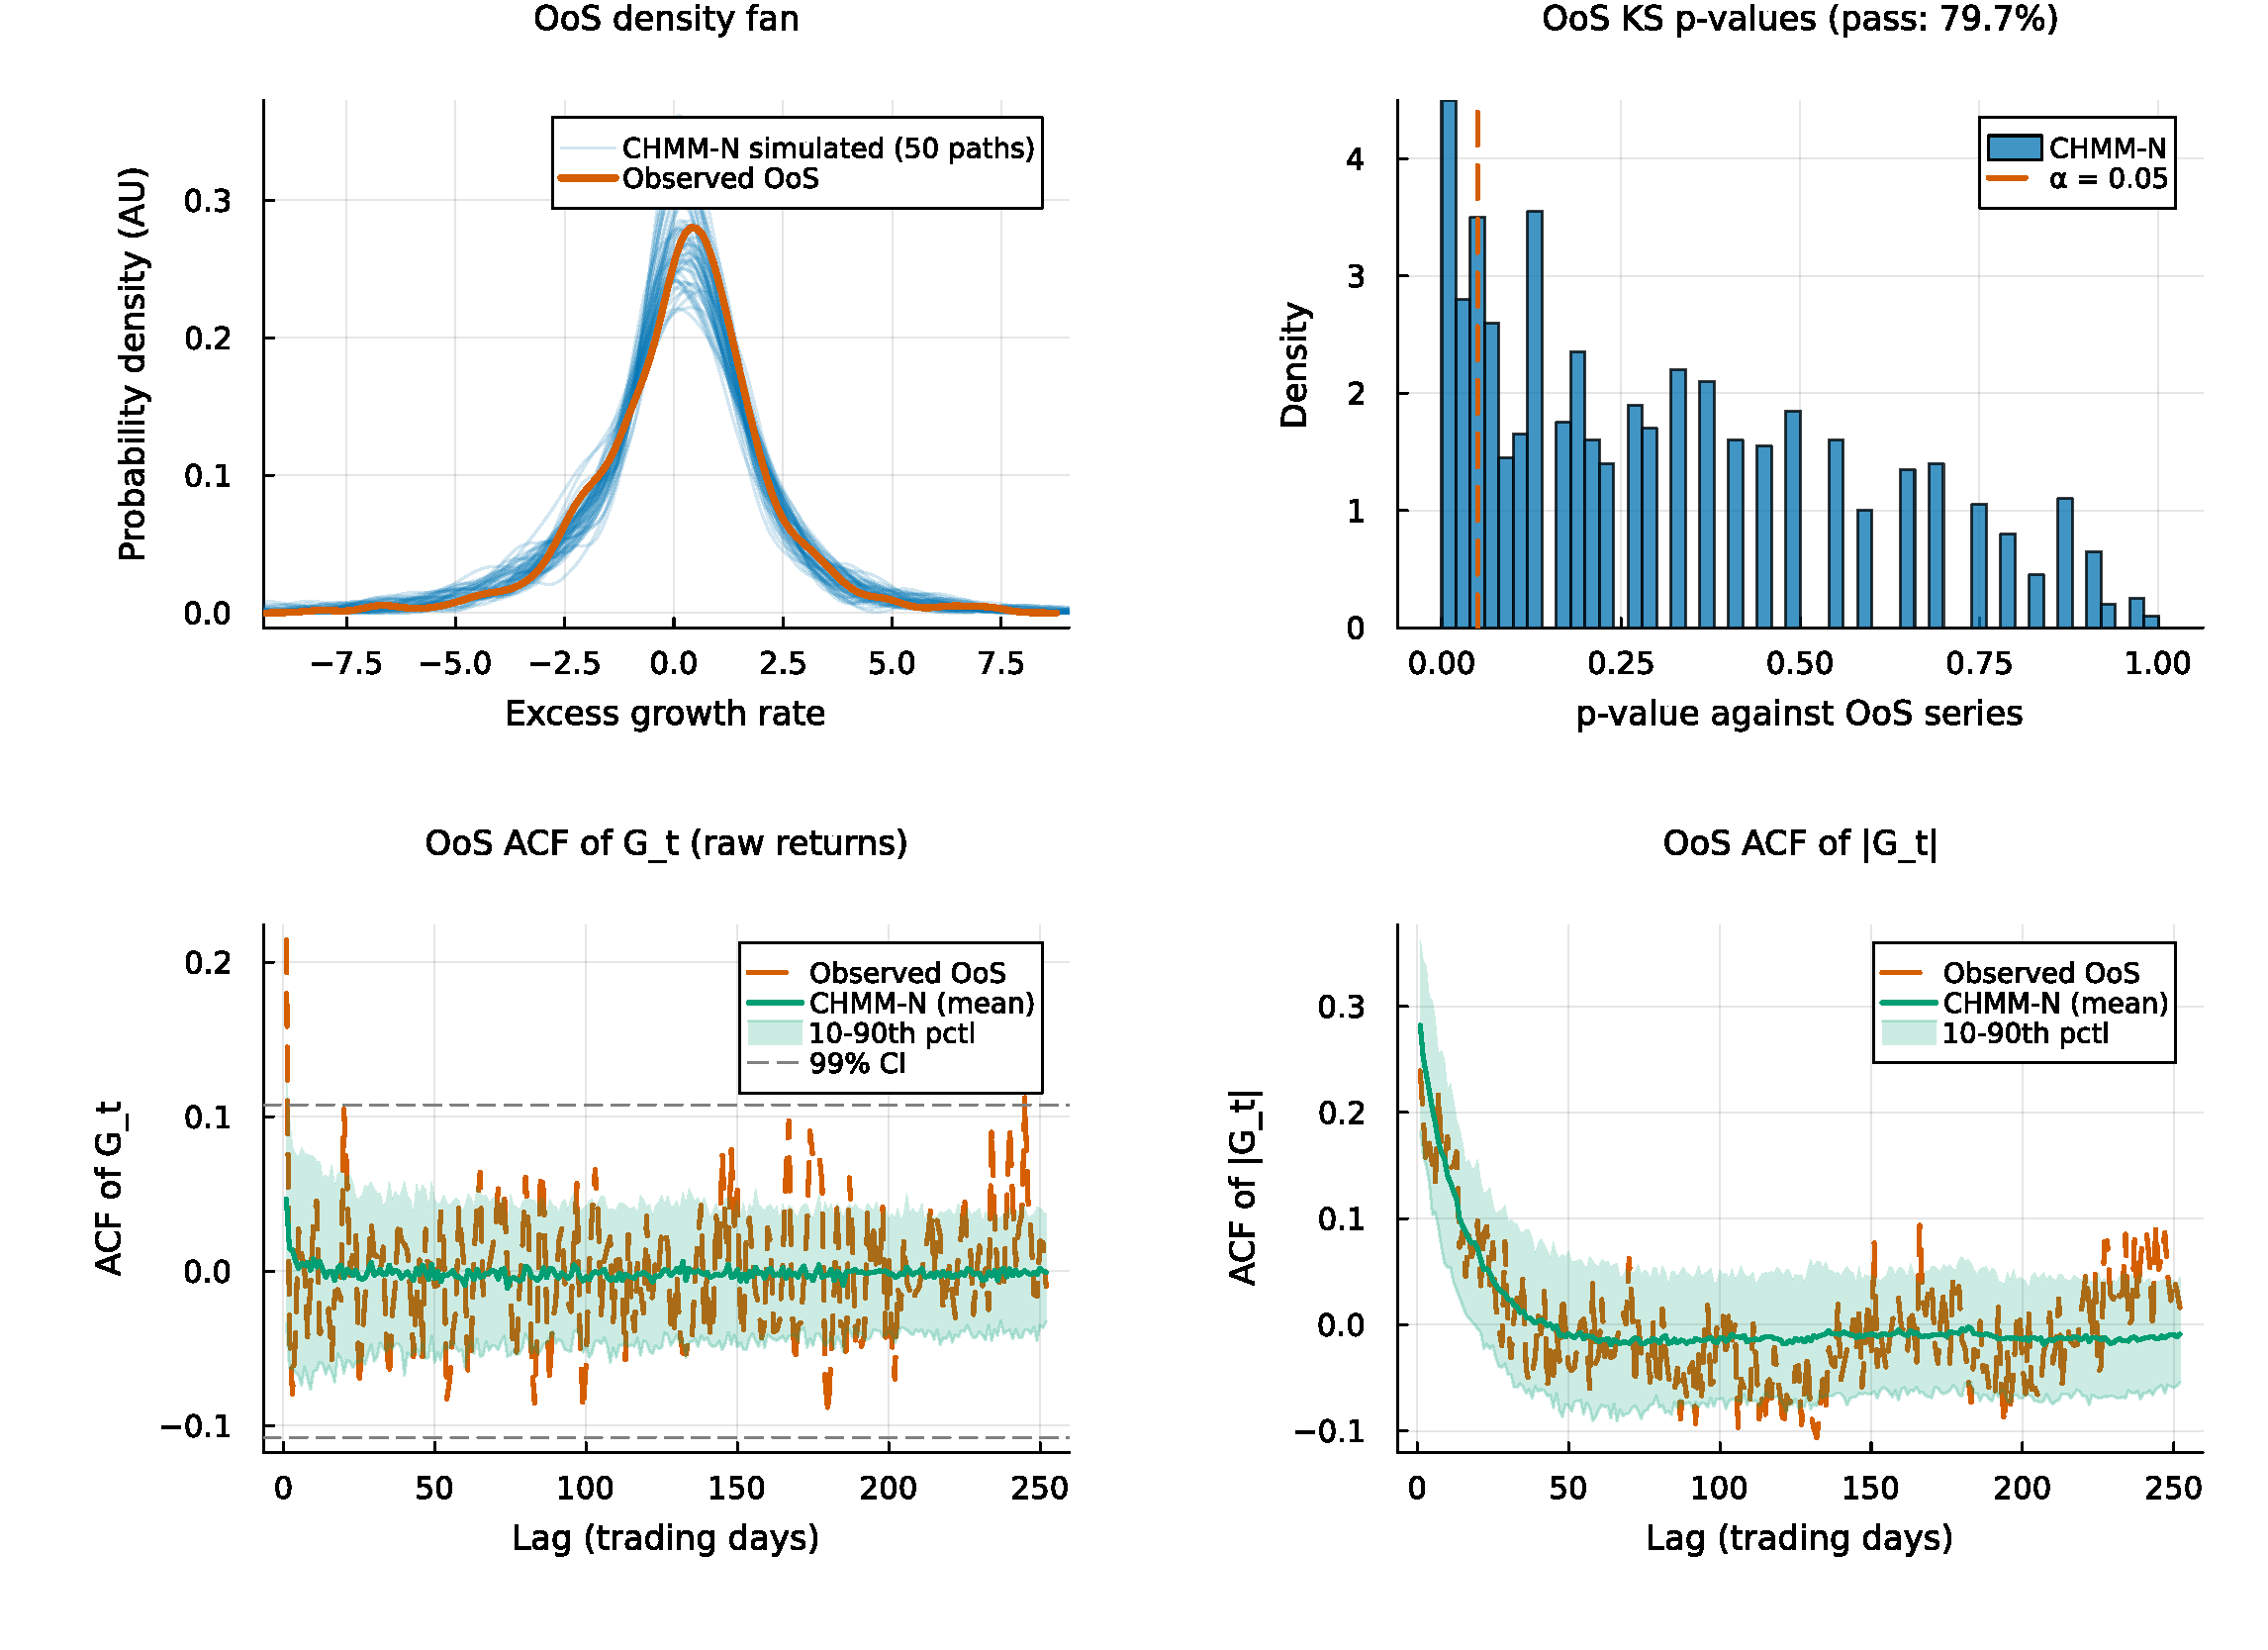
\includegraphics[width=\textwidth]{figs/Fig-4-OoS-Validation-K6.pdf}
\caption{OoS SPY CHMM-N validation at $K = 6$ (Pipeline~A, 1{,}000 simulated paths; panels as in Figure~\ref{fig:oos_validation}).}
\label{fig:k_sweep_oos_k6}
\end{figure}

\begin{figure}[H]
\centering
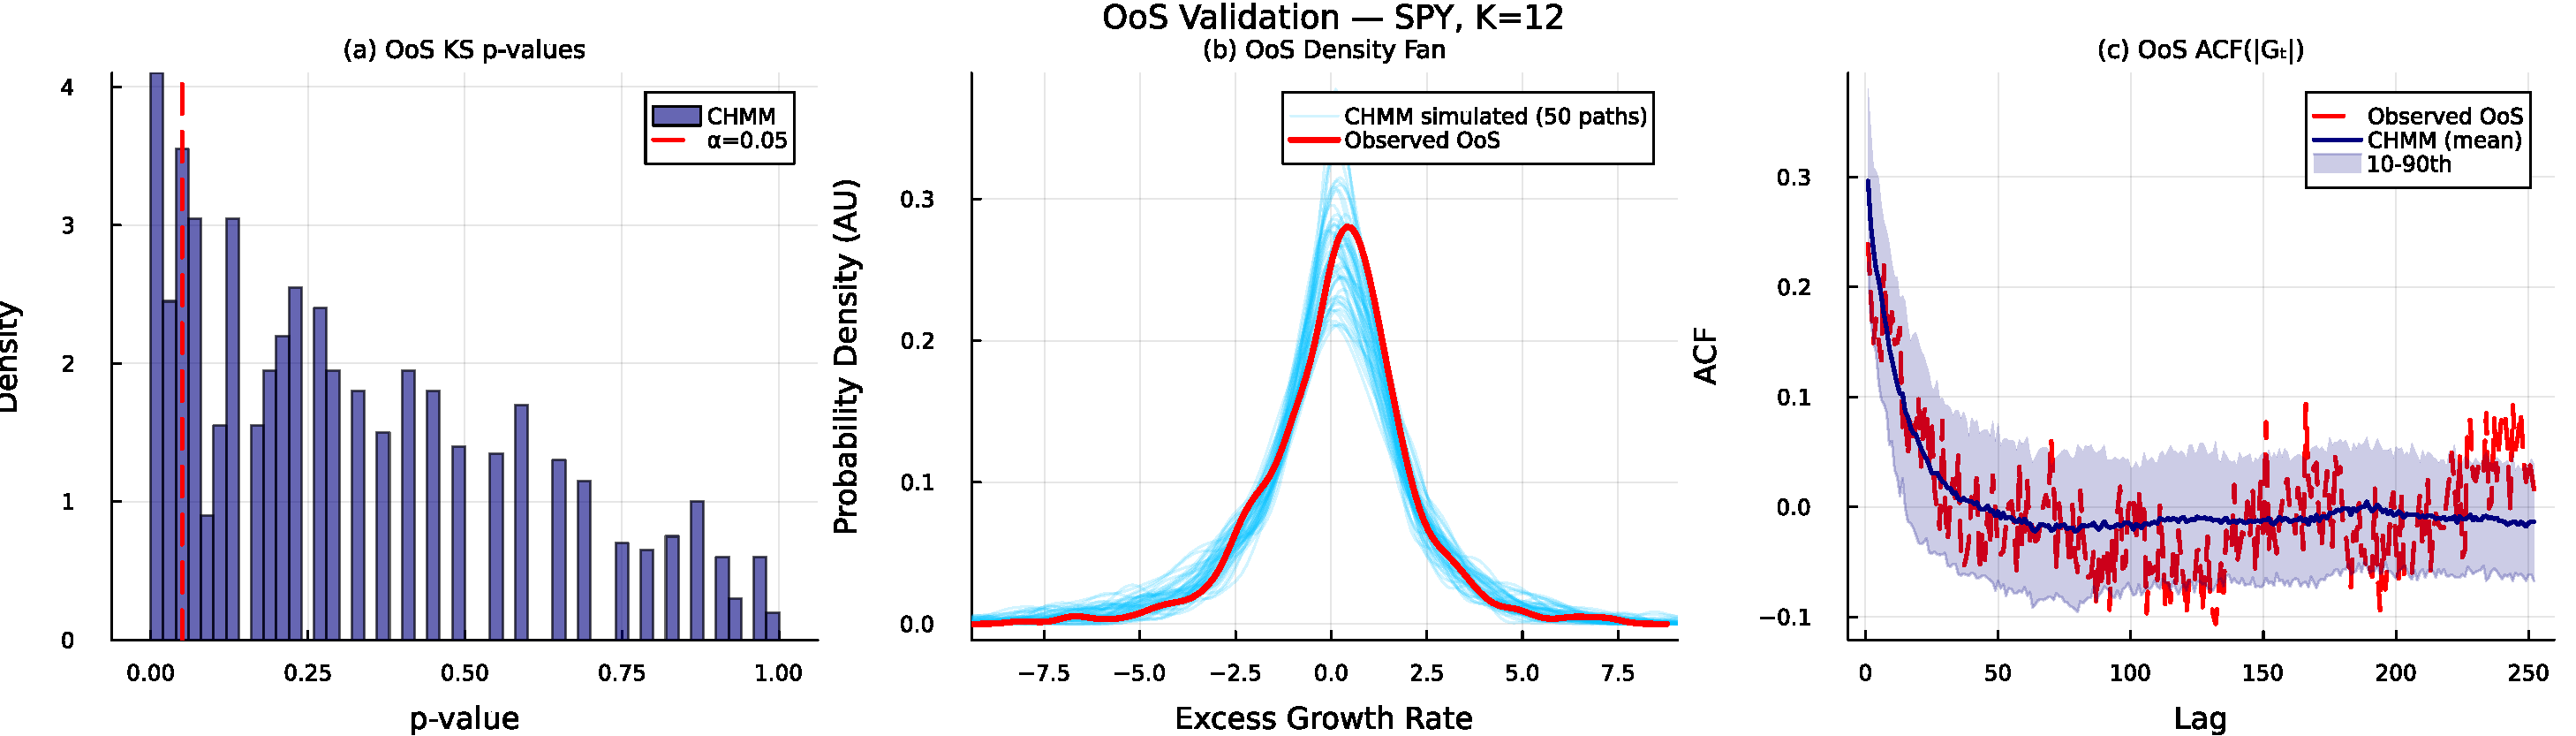
\includegraphics[width=\textwidth]{figs/Fig-4-OoS-Validation-K12.pdf}
\caption{OoS SPY CHMM-N validation at $K = 12$ (Pipeline~A, 1{,}000 simulated paths; panels as in Figure~\ref{fig:oos_validation}).}
\label{fig:k_sweep_oos_k12}
\end{figure}

\begin{figure}[H]
\centering
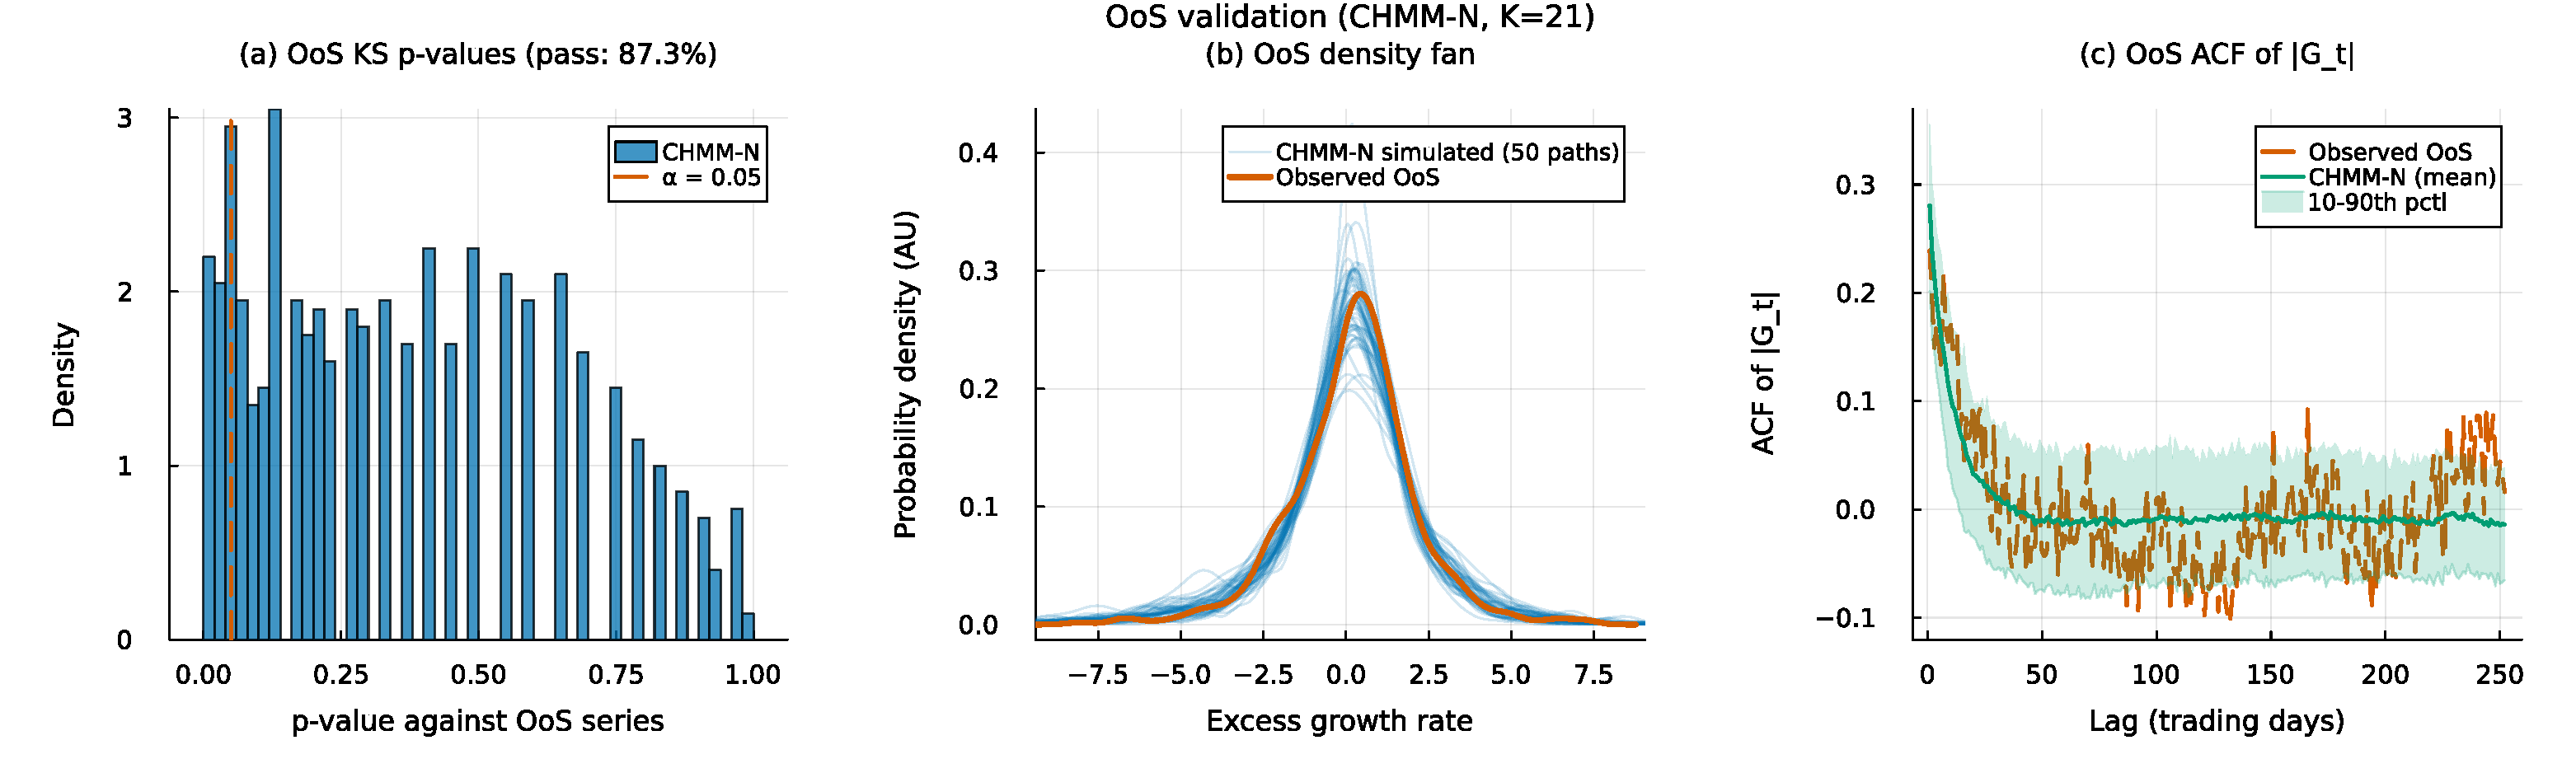
\includegraphics[width=\textwidth]{figs/Fig-4-OoS-Validation-K21.pdf}
\caption{OoS SPY CHMM-N validation at $K = 21$ (Pipeline~A, 1{,}000 simulated paths; panels as in Figure~\ref{fig:oos_validation}).}
\label{fig:k_sweep_oos_k21}
\end{figure}

\subsubsection{\texorpdfstring{Multi-Emission Figures at $K = 18$}{Multi-Emission Figures at K = 18}}
\label{sec:multi_emission_figs}

This appendix reproduces the standard diagnostic suite (emission PDFs, residence times, IS comparison, OoS validation, and convergence) for the two heavy-tailed emission families (CHMM-t and CHMM-L) at the selected state resolution $K = 18$; transition matrices and stationary distributions are discussed in prose only below, since they are visually indistinguishable across families at $K = 18$.
The Gaussian counterparts are already shown as Figures~\ref{fig:is_comparison} and~\ref{fig:oos_validation} in the main text and as Figure~\ref{fig:convergence_all} above in this appendix.
The figures confirm that the shared forward--backward scaffold produces internally-similar regime structure across the three families: the near-diagonal transition band, the $K$-component dense emission cover, the longer central-state residence times, and the monotone log-likelihood convergence are features of the CHMM framework and not of the Gaussian component specifically.

\paragraph{Emission PDFs.}
Figure~\ref{fig:emissions_families} compares the learned $K = 18$ emissions for the three families.
The CHMM-t panel's per-state $\nu_k$ allocation is visible in the narrower modes of certain tail states; the CHMM-L panel's Laplace components have sharper peaks and slower exponential tail decay than the Gaussians.

\begin{figure}[H]
\centering
\begin{subfigure}[b]{0.32\textwidth}
    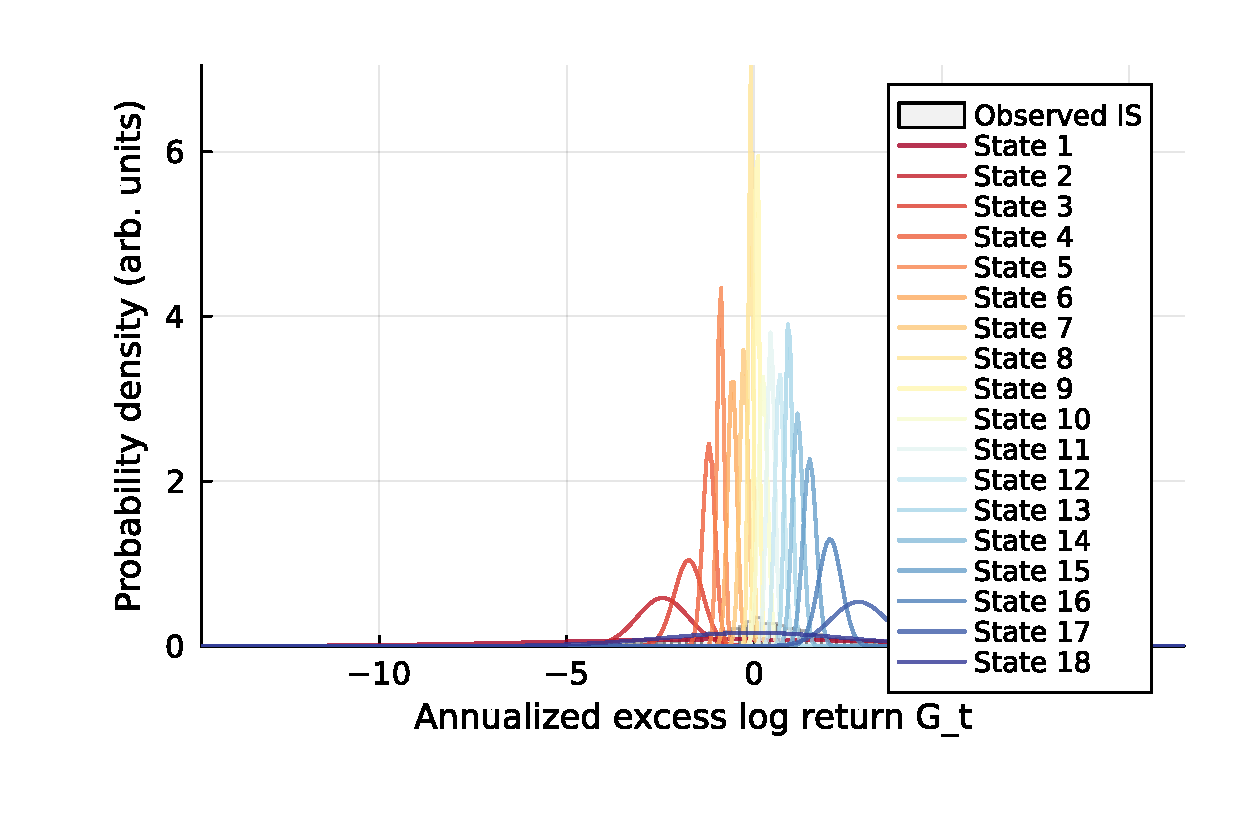
\includegraphics[width=\textwidth]{figs/Fig-Emission-PDFs-K18-N.pdf}
    \caption{CHMM-N (Gaussian)}
\end{subfigure}
\hfill
\begin{subfigure}[b]{0.32\textwidth}
    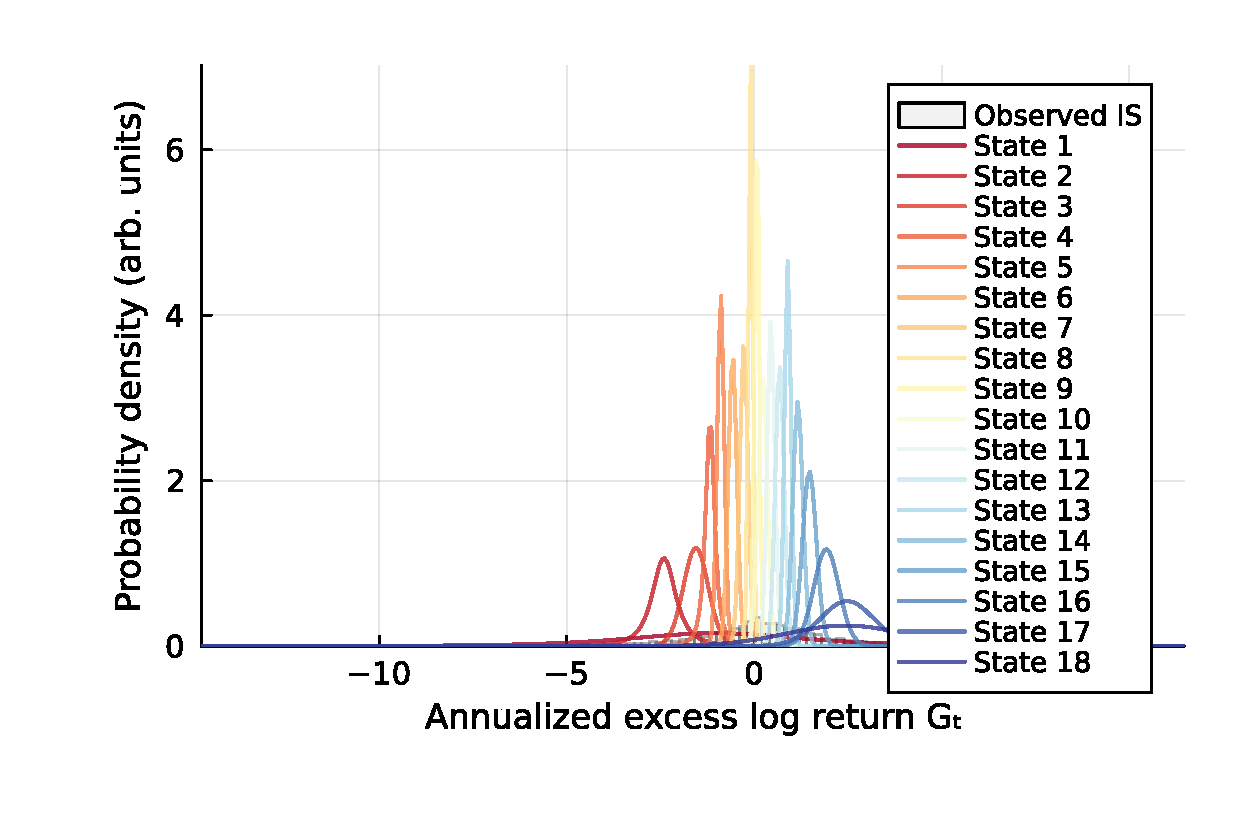
\includegraphics[width=\textwidth]{figs/Fig-Emission-PDFs-K18-t.pdf}
    \caption{CHMM-t (Student-t)}
\end{subfigure}
\hfill
\begin{subfigure}[b]{0.32\textwidth}
    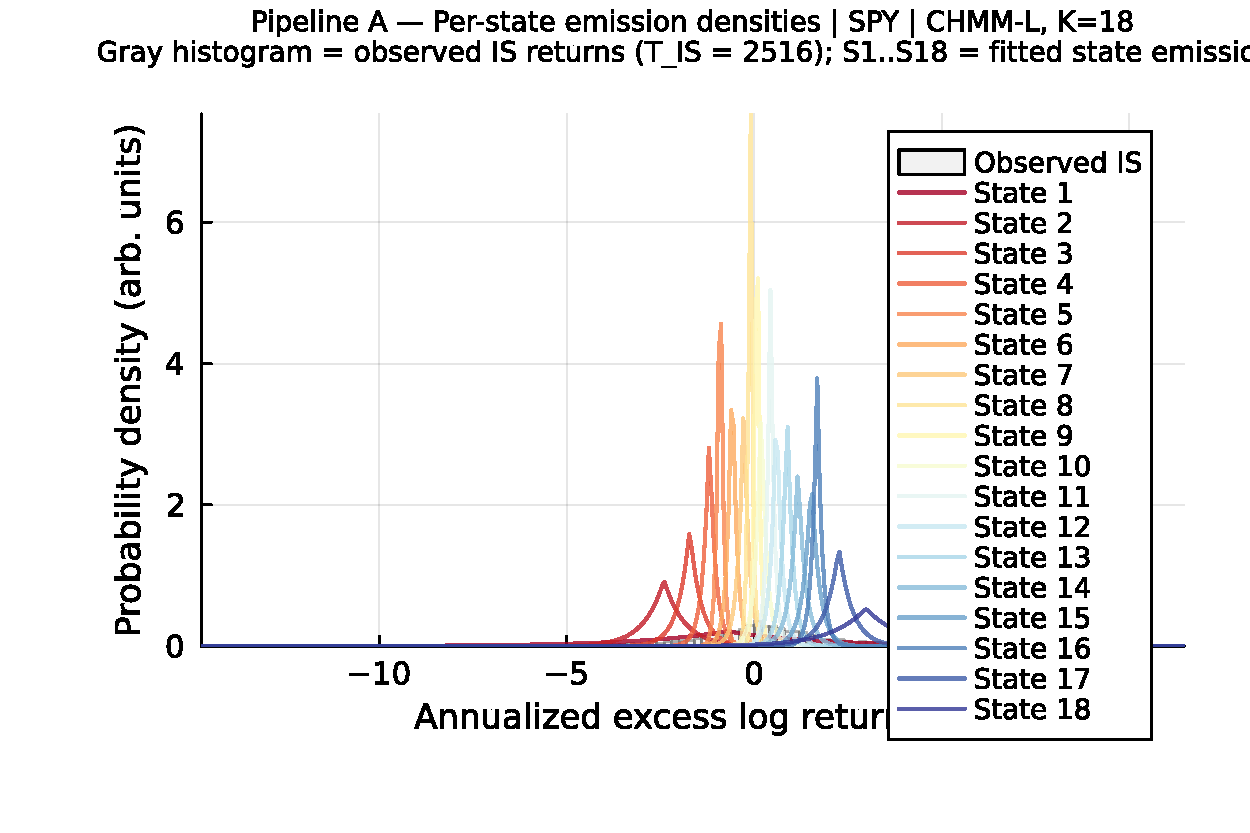
\includegraphics[width=\textwidth]{figs/Fig-Emission-PDFs-K18-L.pdf}
    \caption{CHMM-L (Laplace)}
\end{subfigure}
\caption{Learned emission distributions at $K = 18$ across the three emission families (CHMM-N Gaussian, CHMM-t Student-t with per-state $\nu_k$, CHMM-L Laplace), overlaid on the observed SPY IS return histogram (Pipeline~A). Heavier-tailed emission families (t, L) give individual components more tail mass, which is what closes the kurtosis gap of the Gaussian CHMM.}
\label{fig:emissions_families}
\end{figure}

\paragraph{Transition matrices and stationary distributions.}
The $K = 18$ transition matrices and stationary distributions learned under CHMM-t and CHMM-L are visually indistinguishable from their CHMM-N counterparts: the near-diagonal band, the magnitude of self-transition probabilities, and the mass concentration at central states are features of the regime structure, not the emission family. This is consistent with the ACF-MAE being stable across the family axis (Table~\ref{tab:sensitivity_multi}). The per-family residence times $\tau_k = 1/(1 - T_{kk})$, which magnify small differences in the self-transition probabilities each family recovers, are compared in Figure~\ref{fig:residence_families}.

\begin{figure}[H]
\centering
\begin{subfigure}[b]{0.32\textwidth}
    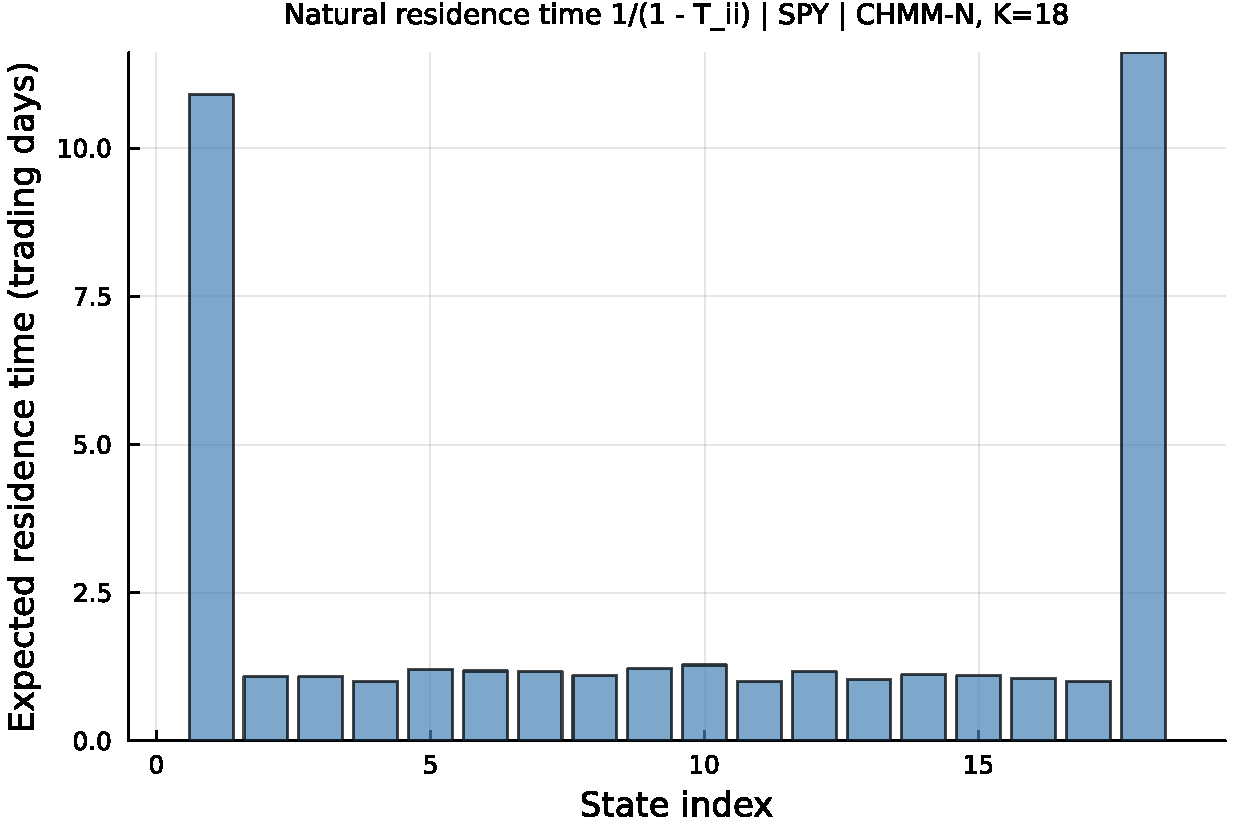
\includegraphics[width=\textwidth]{figs/Fig-Residence-Times-K18-N.pdf}
    \caption{CHMM-N}
\end{subfigure}
\hfill
\begin{subfigure}[b]{0.32\textwidth}
    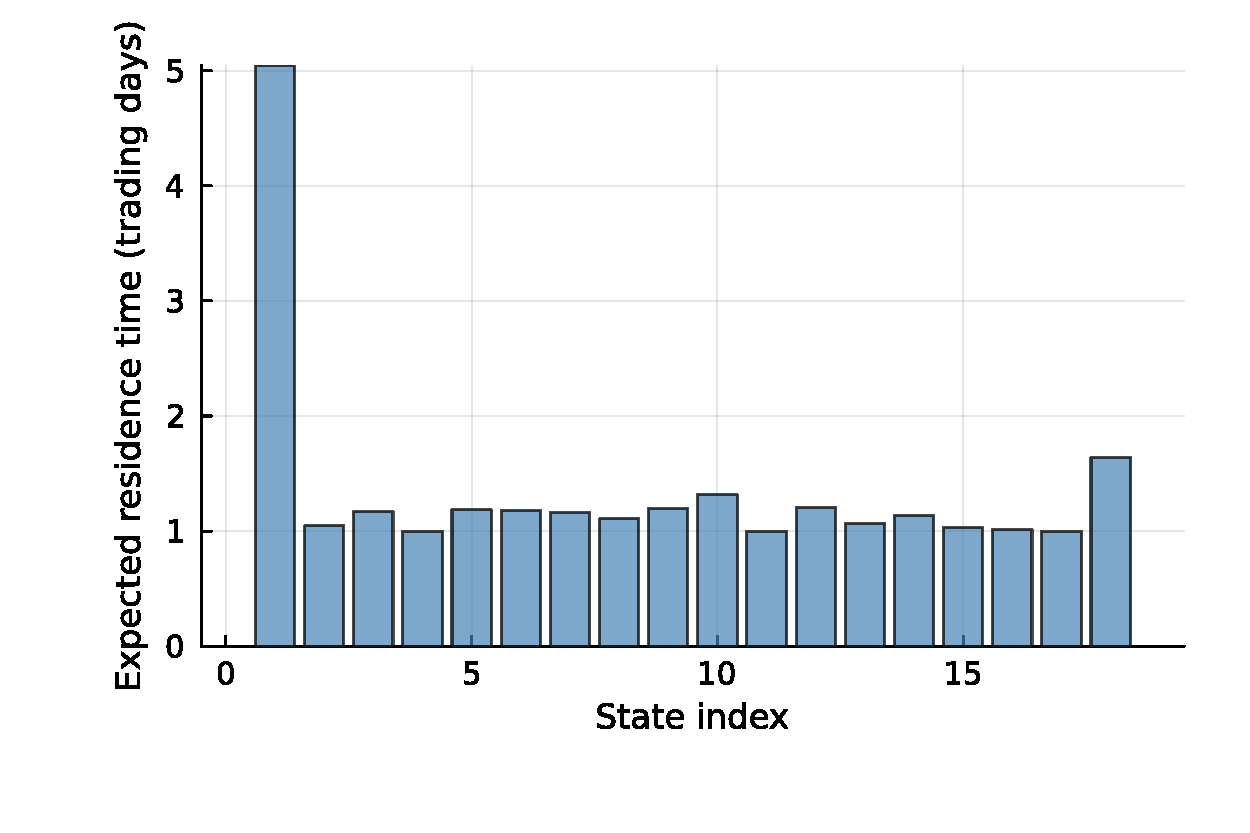
\includegraphics[width=\textwidth]{figs/Fig-Residence-Times-K18-t.pdf}
    \caption{CHMM-t}
\end{subfigure}
\hfill
\begin{subfigure}[b]{0.32\textwidth}
    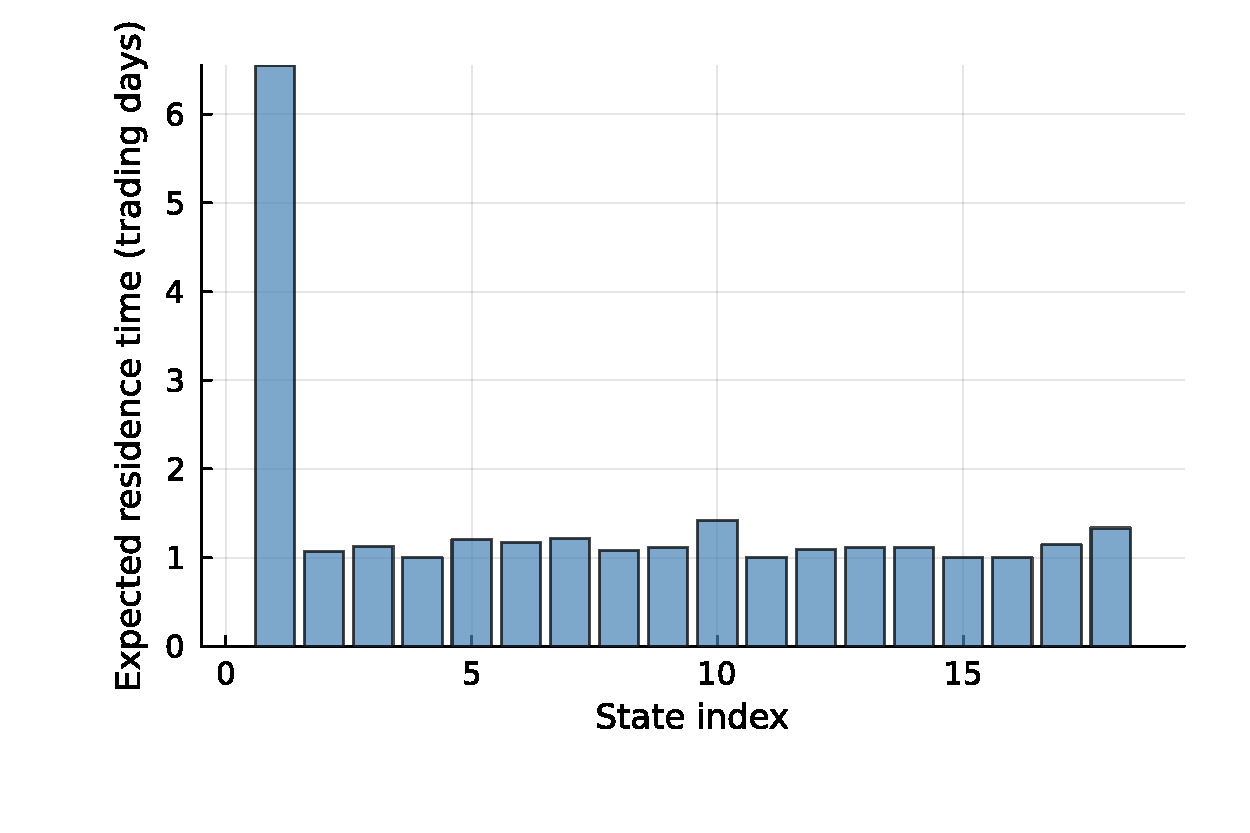
\includegraphics[width=\textwidth]{figs/Fig-Residence-Times-K18-L.pdf}
    \caption{CHMM-L}
\end{subfigure}
\caption{Natural residence times $\tau_k = 1/(1 - T_{kk})$ at $K = 18$ for the SPY IS fit (Pipeline~A) across the three emission families (CHMM-N Gaussian, CHMM-t Student-t, CHMM-L Laplace).}
\label{fig:residence_families}
\end{figure}

\paragraph{IS comparison.}
Figures~\ref{fig:is_families}--\ref{fig:is_families_L} reproduce the three-panel IS comparison (density, ACF of $|G_t|$, tail Q-Q) at $K = 18$ for the two heavy-tailed families; the CHMM-N panel is Figure~\ref{fig:is_comparison} in the main text.

\begin{figure}[H]
\centering
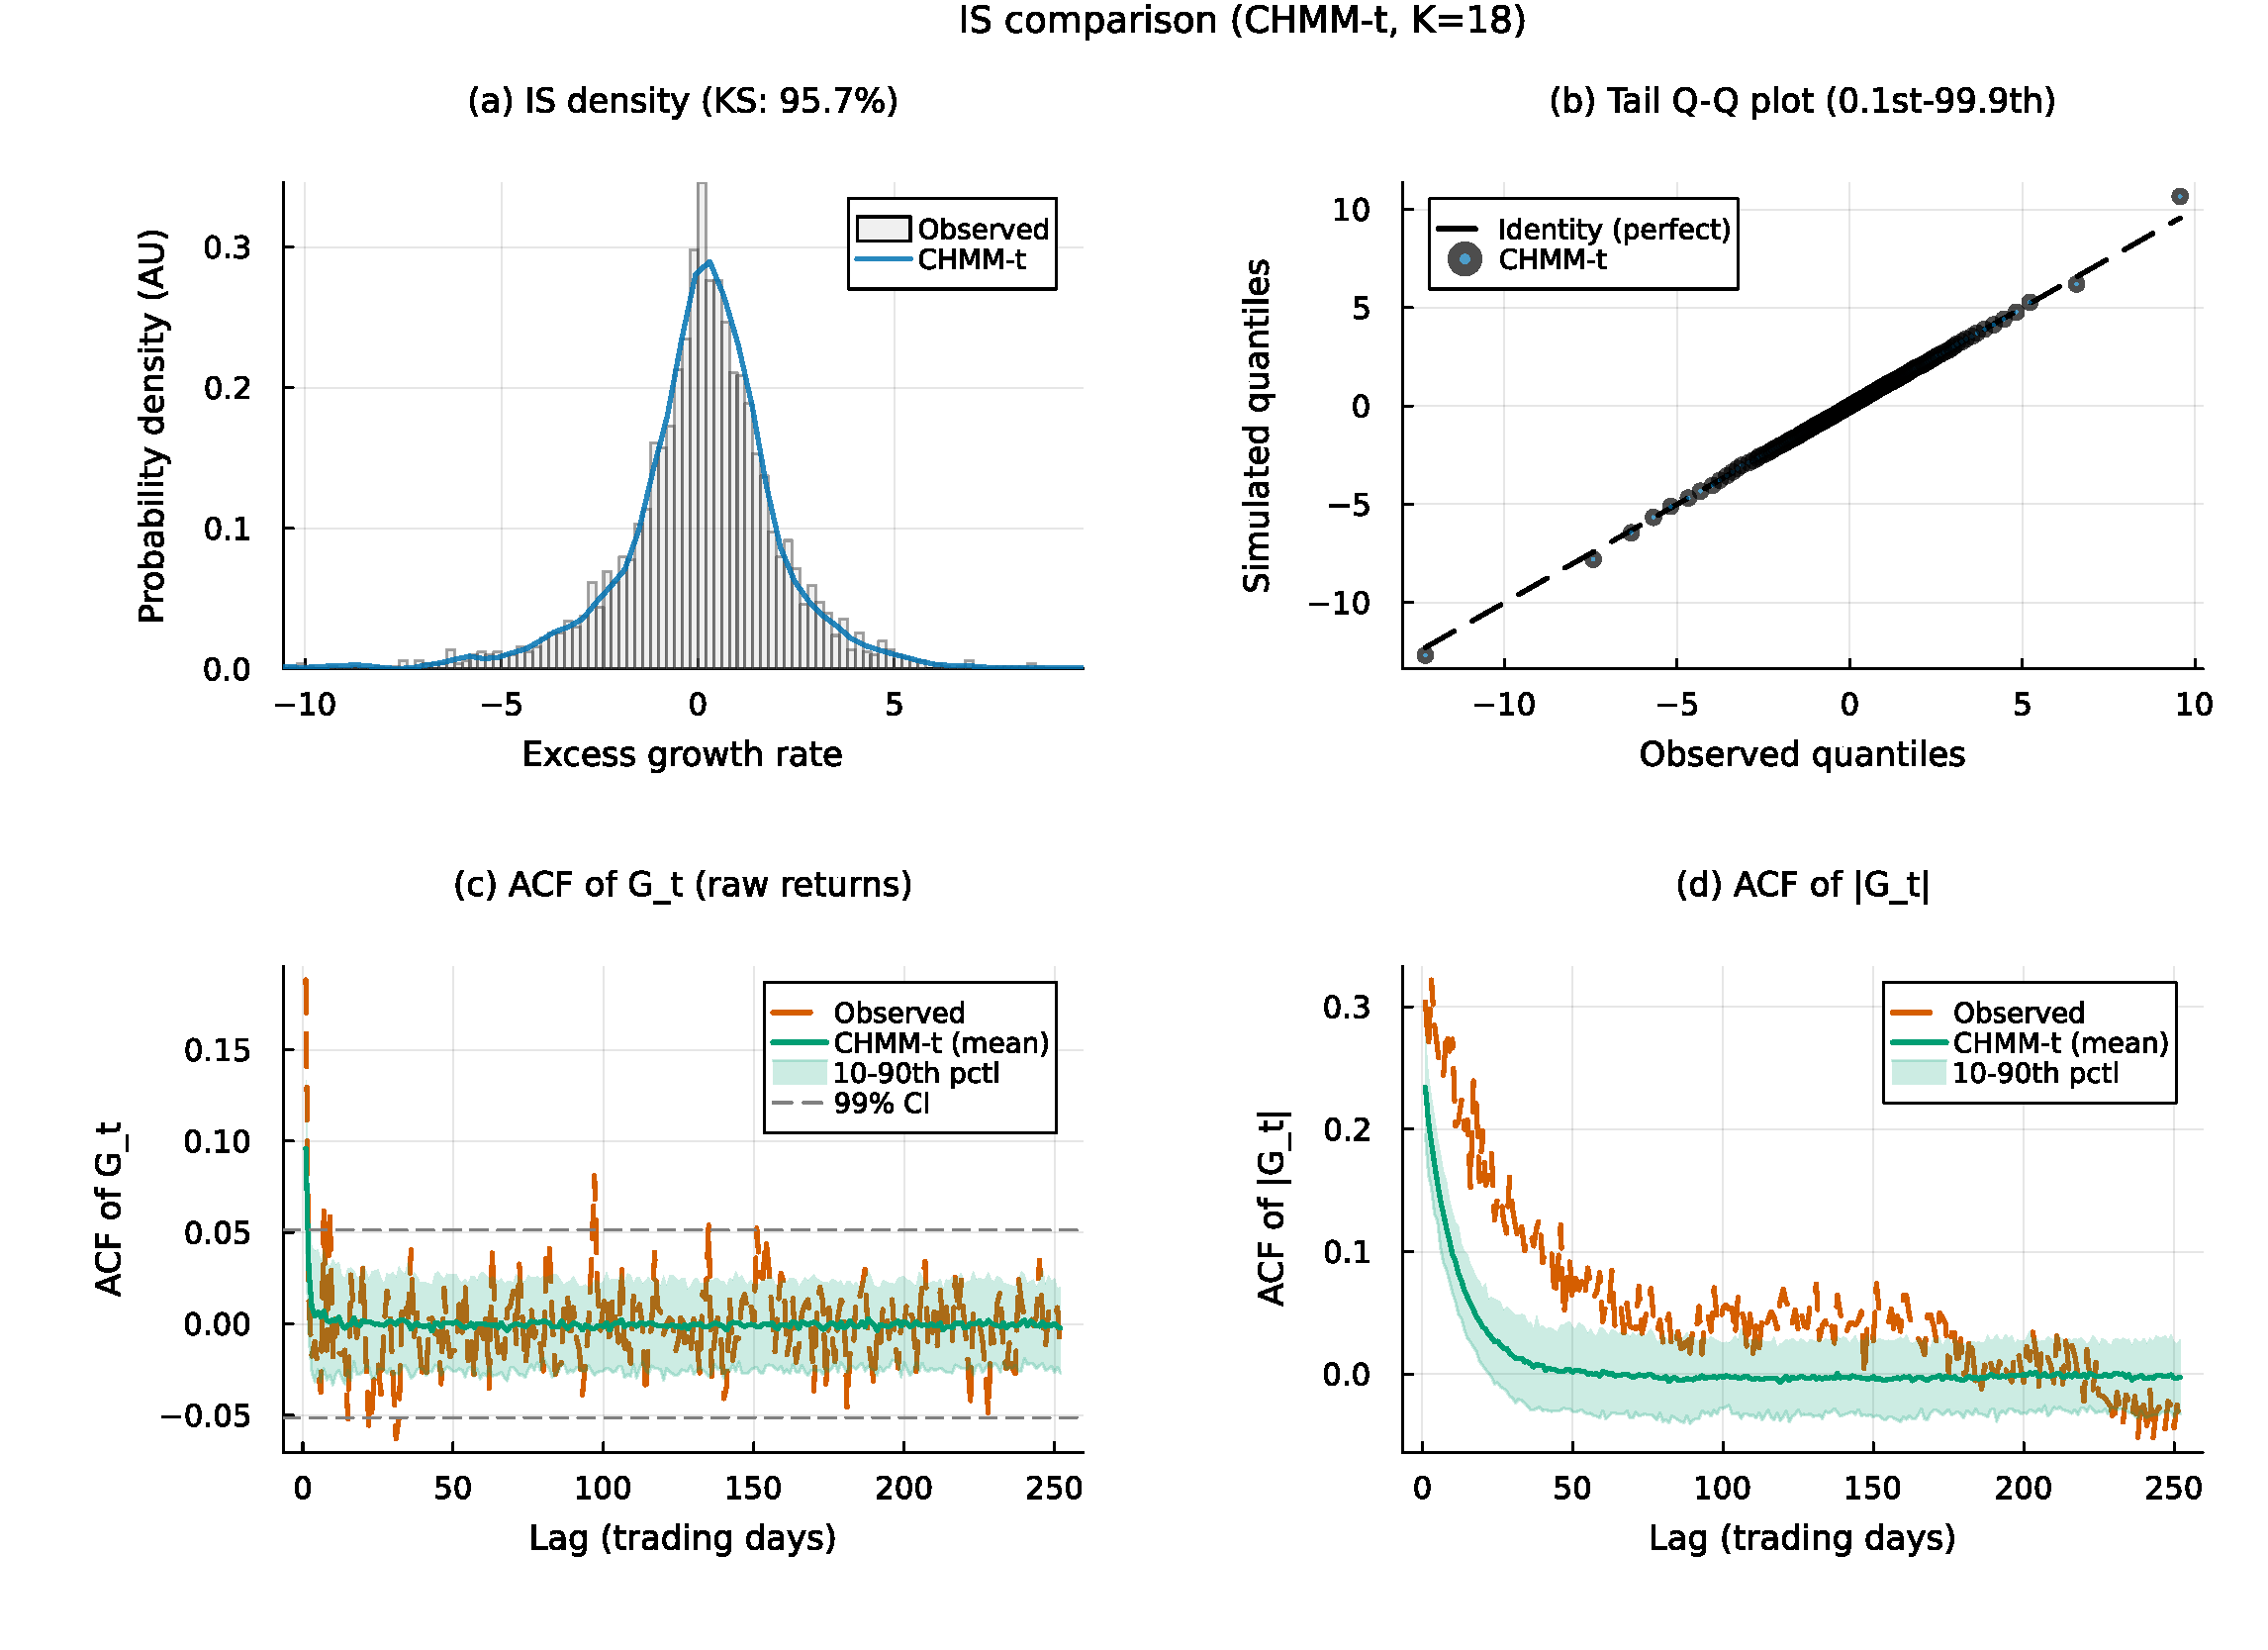
\includegraphics[width=\textwidth]{figs/Fig-3-IS-Comparison-K18-t.pdf}
\caption{IS SPY model comparison at $K = 18$ for CHMM-t Student-t emissions (Pipeline~A, 1{,}000 simulated paths). Panels show (a) marginal density with KS pass rate, (b) ACF of $|G_t|$, and (c) tail Q-Q plot. The CHMM-N counterpart is Figure~\ref{fig:is_comparison}; the CHMM-L counterpart is Figure~\ref{fig:is_families_L}.}
\label{fig:is_families}
\end{figure}

\begin{figure}[H]
\centering
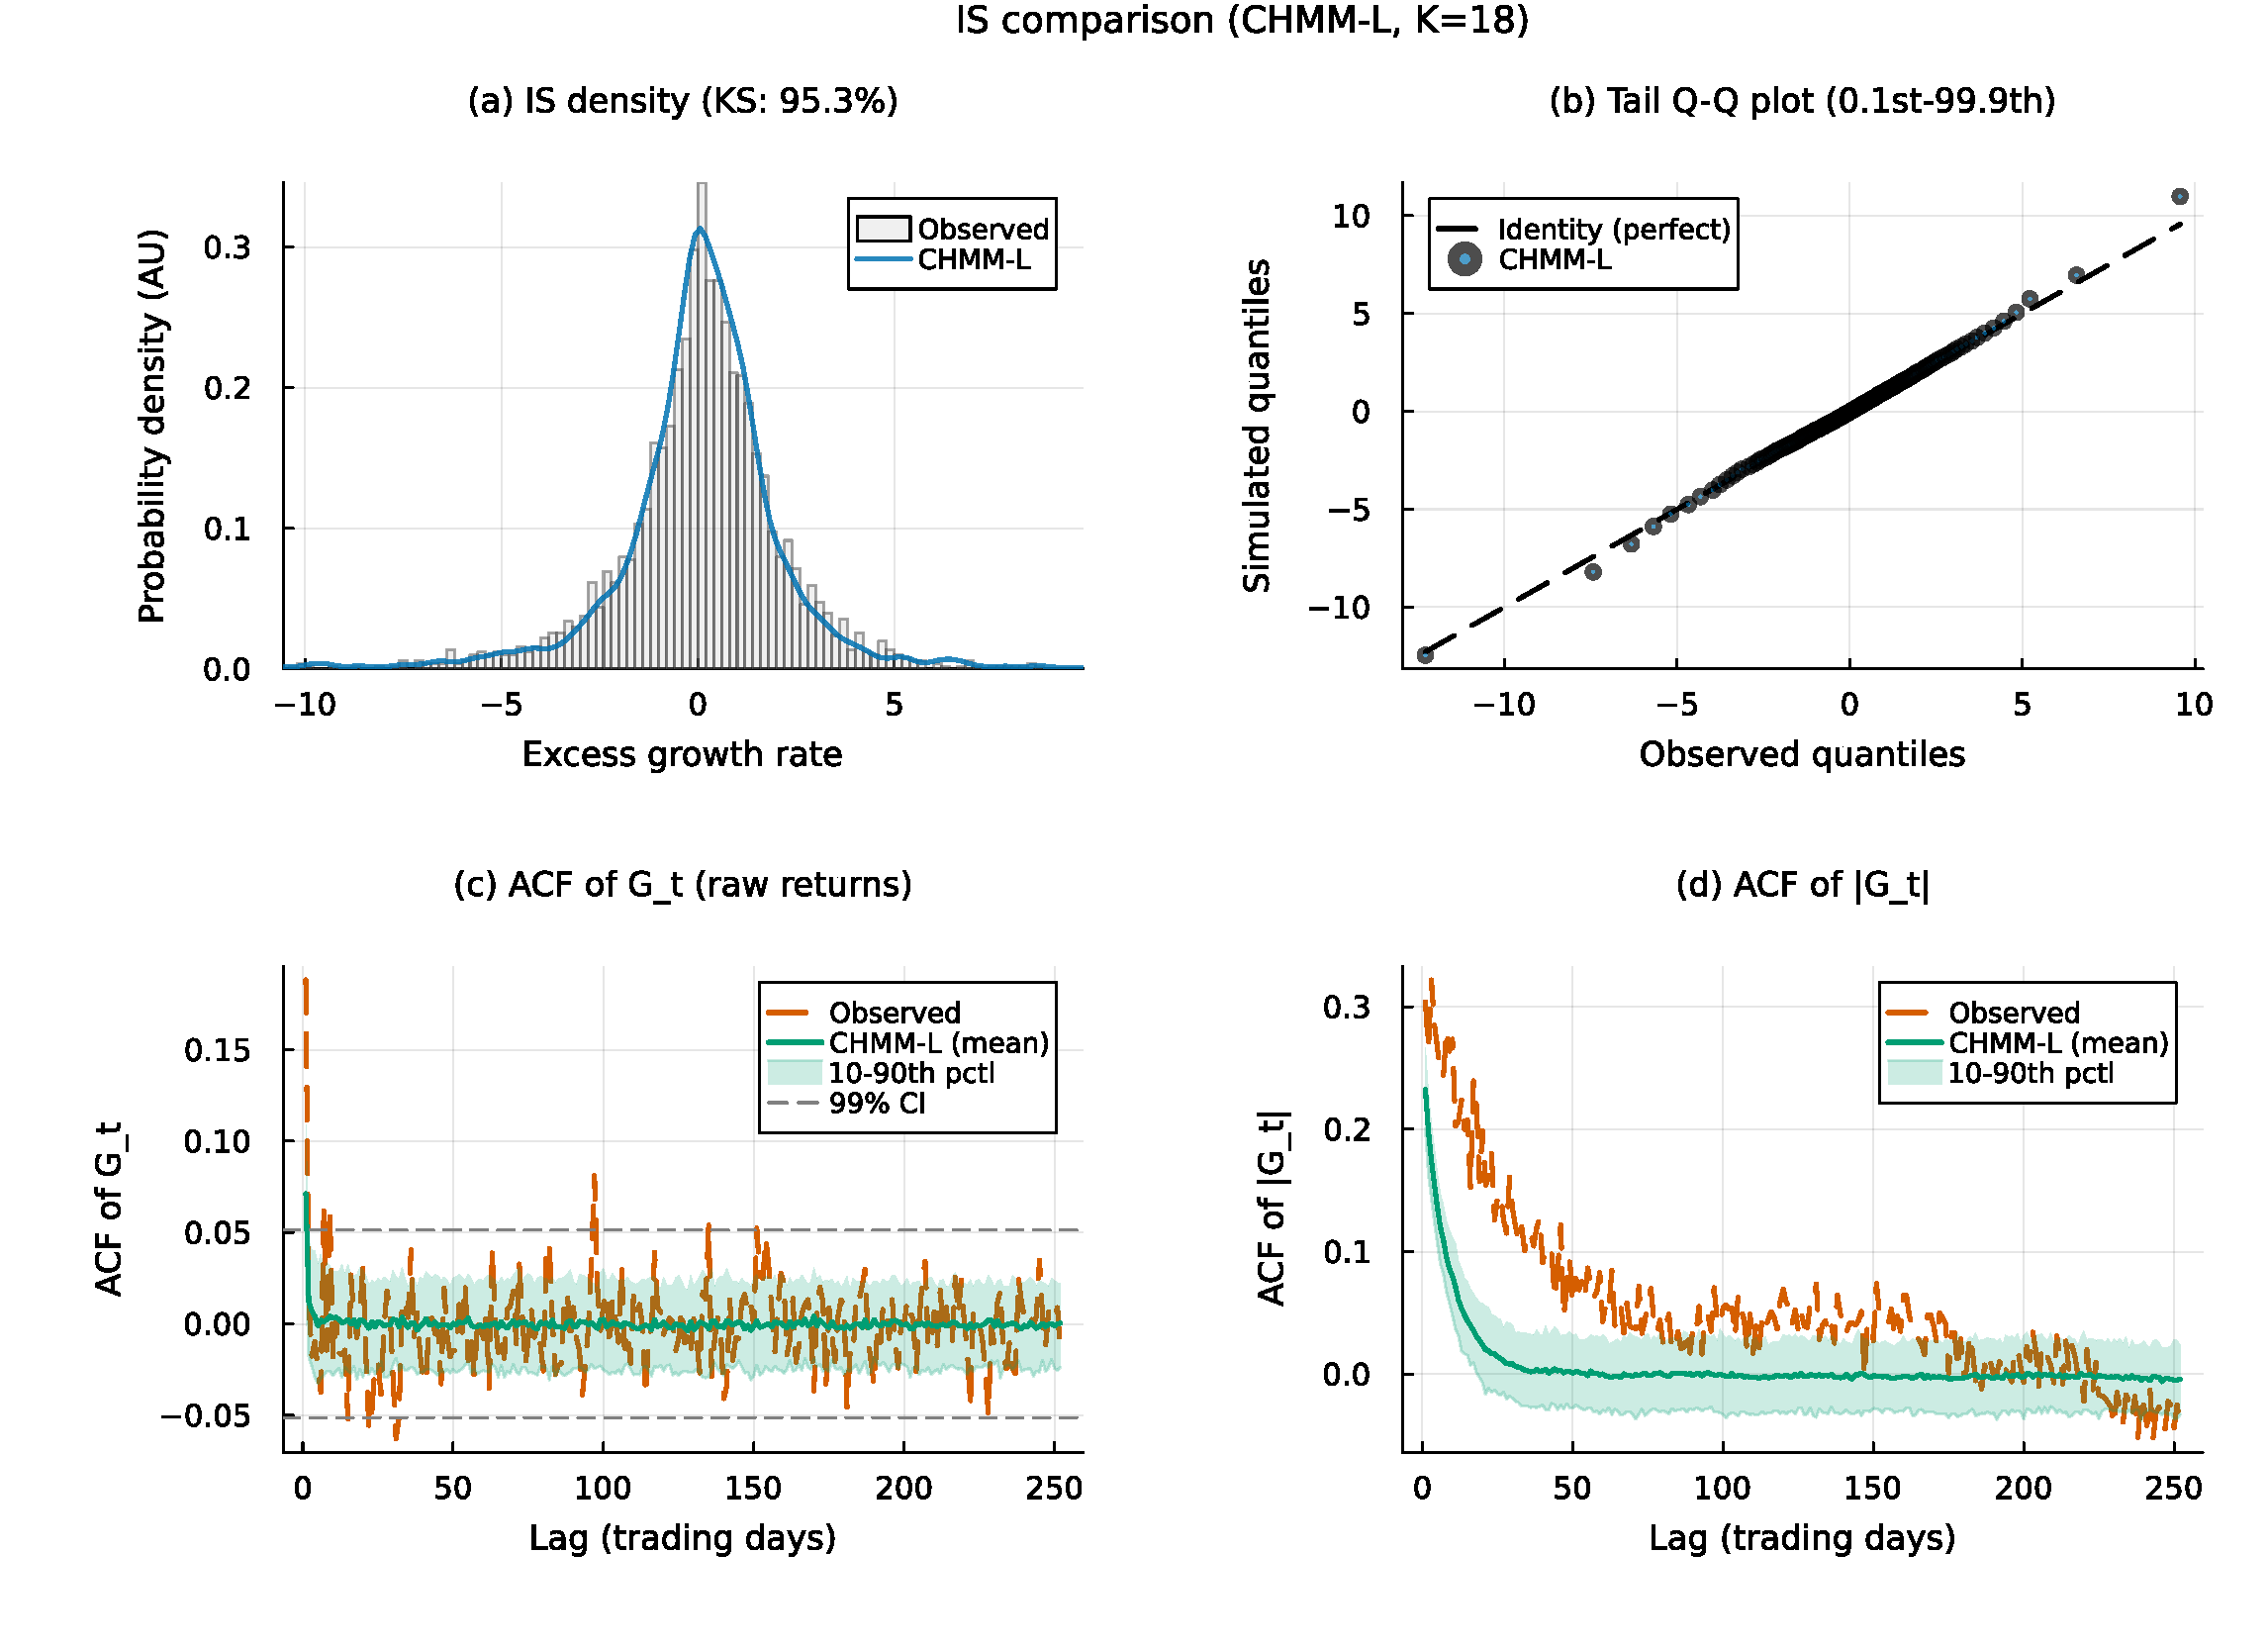
\includegraphics[width=\textwidth]{figs/Fig-3-IS-Comparison-K18-L.pdf}
\caption{IS SPY model comparison at $K = 18$ for CHMM-L Laplace emissions (Pipeline~A, 1{,}000 simulated paths). Panels as in Figure~\ref{fig:is_families}.}
\label{fig:is_families_L}
\end{figure}

\paragraph{OoS validation.}
Figures~\ref{fig:oos_families}--\ref{fig:oos_families_L} show the OoS validation panels for CHMM-t and CHMM-L at $K = 18$.
The CHMM-t panel demonstrates the OoS kurtosis alignment noted in the main text (simulated 6.40 vs.\ observed 6.24), and the CHMM-L panel shows the tighter density fan produced by the heavier Laplace tails relative to the Gaussian.

\begin{figure}[H]
\centering
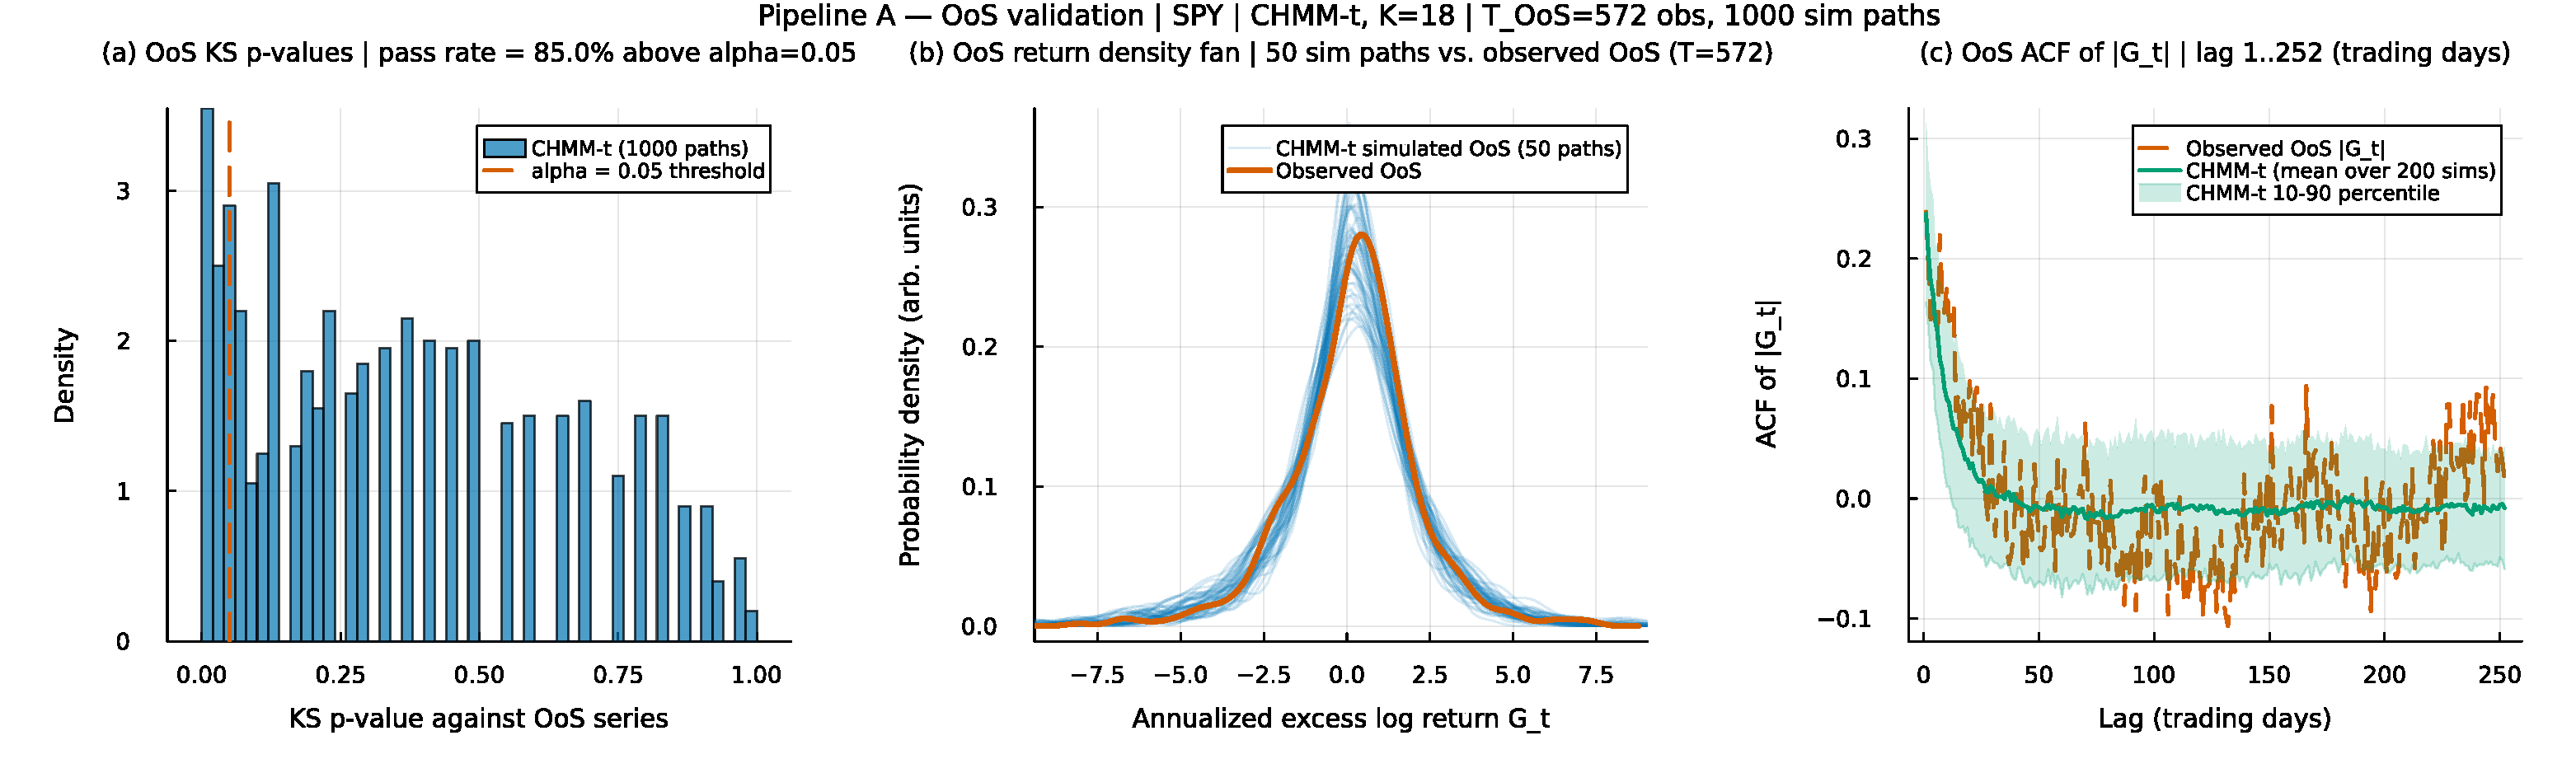
\includegraphics[width=\textwidth]{figs/Fig-4-OoS-Validation-K18-t.pdf}
\caption{OoS SPY validation at $K = 18$ for CHMM-t Student-t emissions (Pipeline~A, 1{,}000 simulated paths). Panels show (a) KS $p$-values, (b) OoS density fan, and (c) OoS ACF of $|G_t|$. The CHMM-N counterpart is Figure~\ref{fig:oos_validation}; the CHMM-L counterpart is Figure~\ref{fig:oos_families_L}.}
\label{fig:oos_families}
\end{figure}

\begin{figure}[H]
\centering
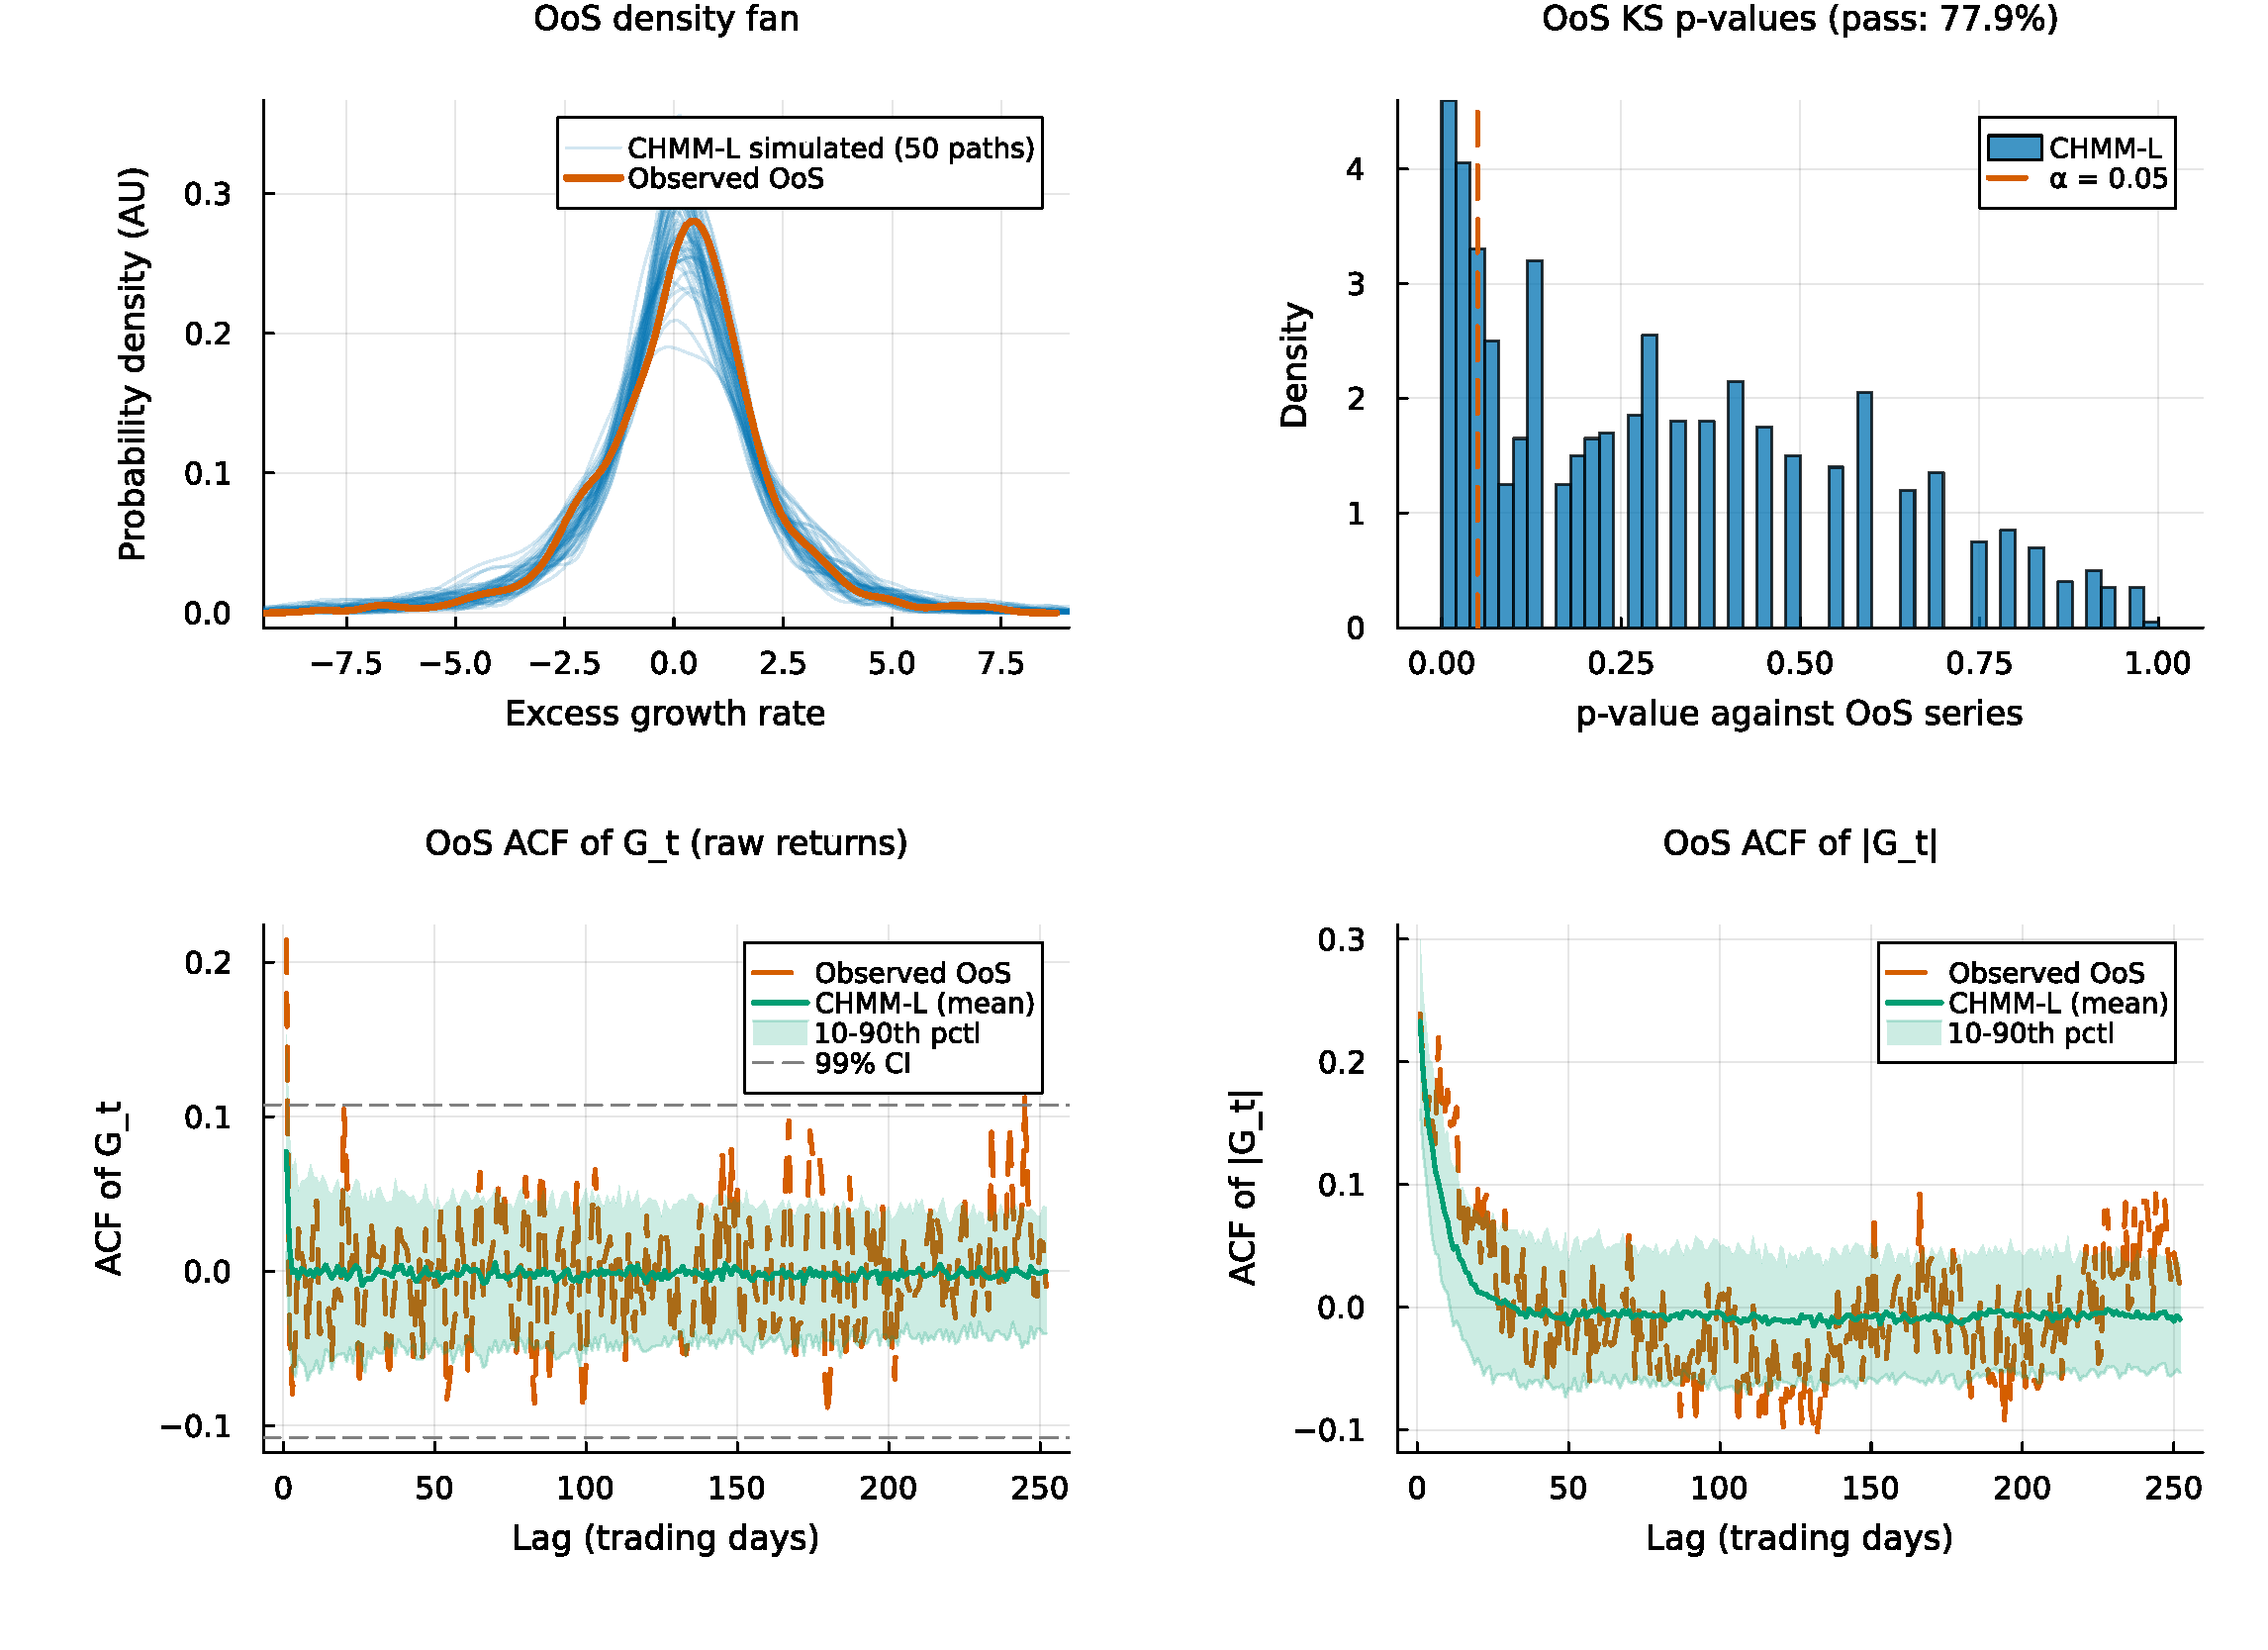
\includegraphics[width=\textwidth]{figs/Fig-4-OoS-Validation-K18-L.pdf}
\caption{OoS SPY validation at $K = 18$ for CHMM-L Laplace emissions (Pipeline~A, 1{,}000 simulated paths). Panels as in Figure~\ref{fig:oos_families}.}
\label{fig:oos_families_L}
\end{figure}

\paragraph{Convergence.}
Figure~\ref{fig:convergence_families} shows the Baum-Welch / ECM / weighted-EM log-likelihood histories at $K = 18$ for all three families.
The CHMM-t and CHMM-L curves inherit the monotone increase of the classical EM guarantee; the CHMM-t curve has a slightly longer pre-plateau phase because each ECM sub-iteration refines $\nu_k$ with a golden-section search.

\begin{figure}[H]
\centering
\begin{subfigure}[b]{0.32\textwidth}
    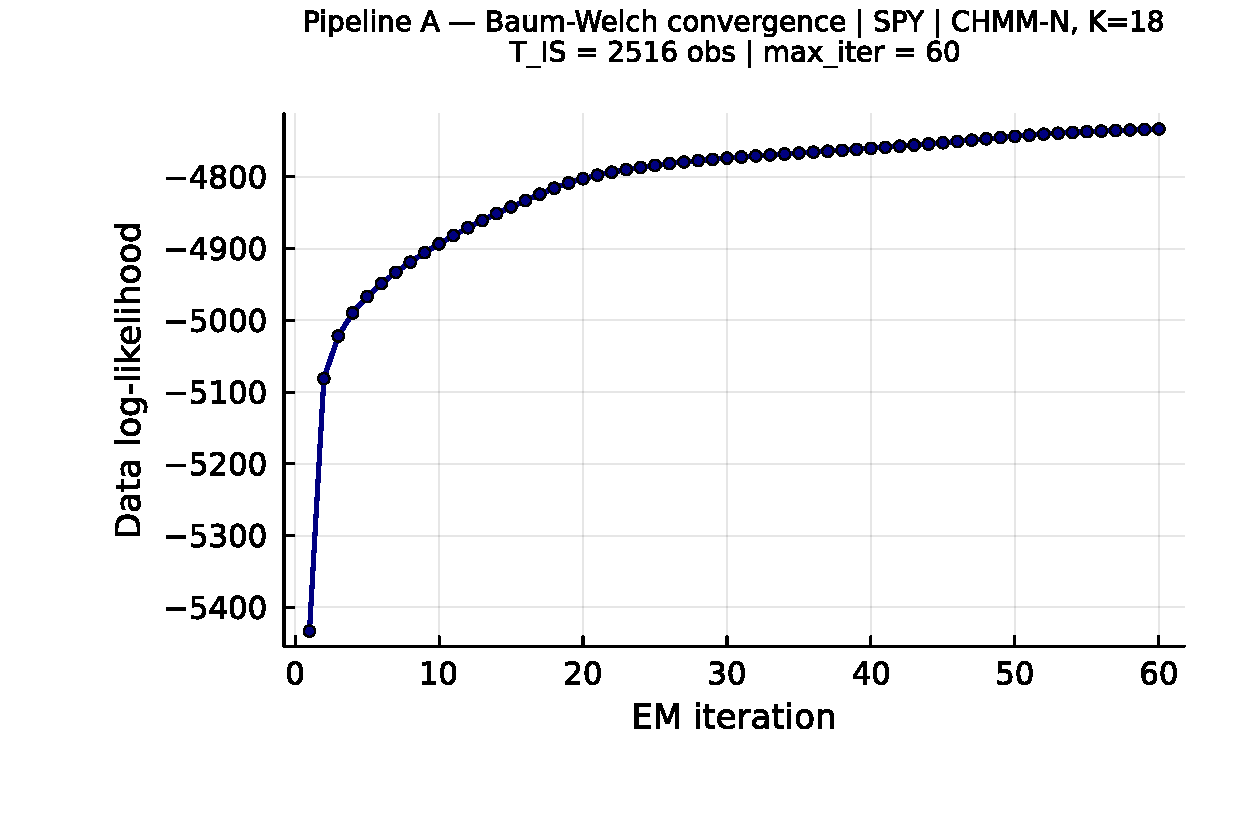
\includegraphics[width=\textwidth]{figs/Fig-Convergence-K18-N.pdf}
    \caption{CHMM-N}
\end{subfigure}
\hfill
\begin{subfigure}[b]{0.32\textwidth}
    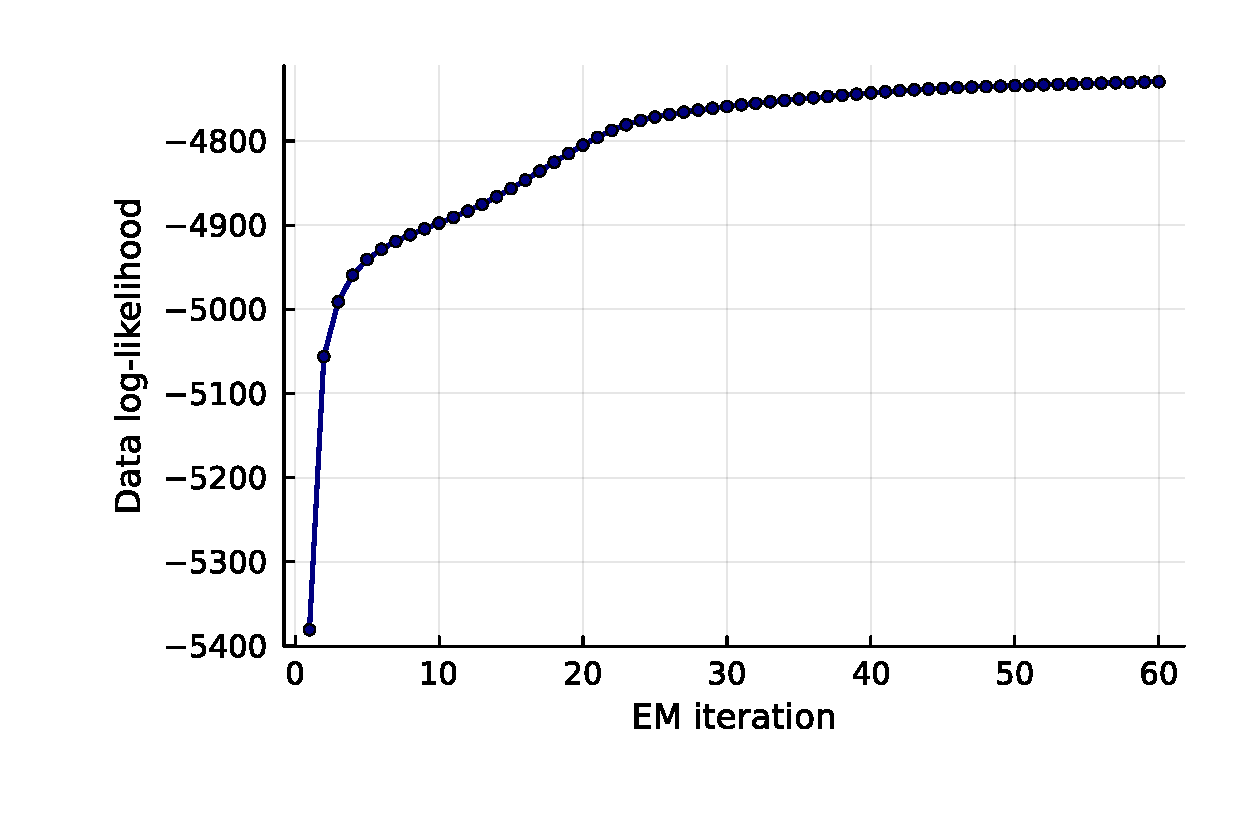
\includegraphics[width=\textwidth]{figs/Fig-Convergence-K18-t.pdf}
    \caption{CHMM-t}
\end{subfigure}
\hfill
\begin{subfigure}[b]{0.32\textwidth}
    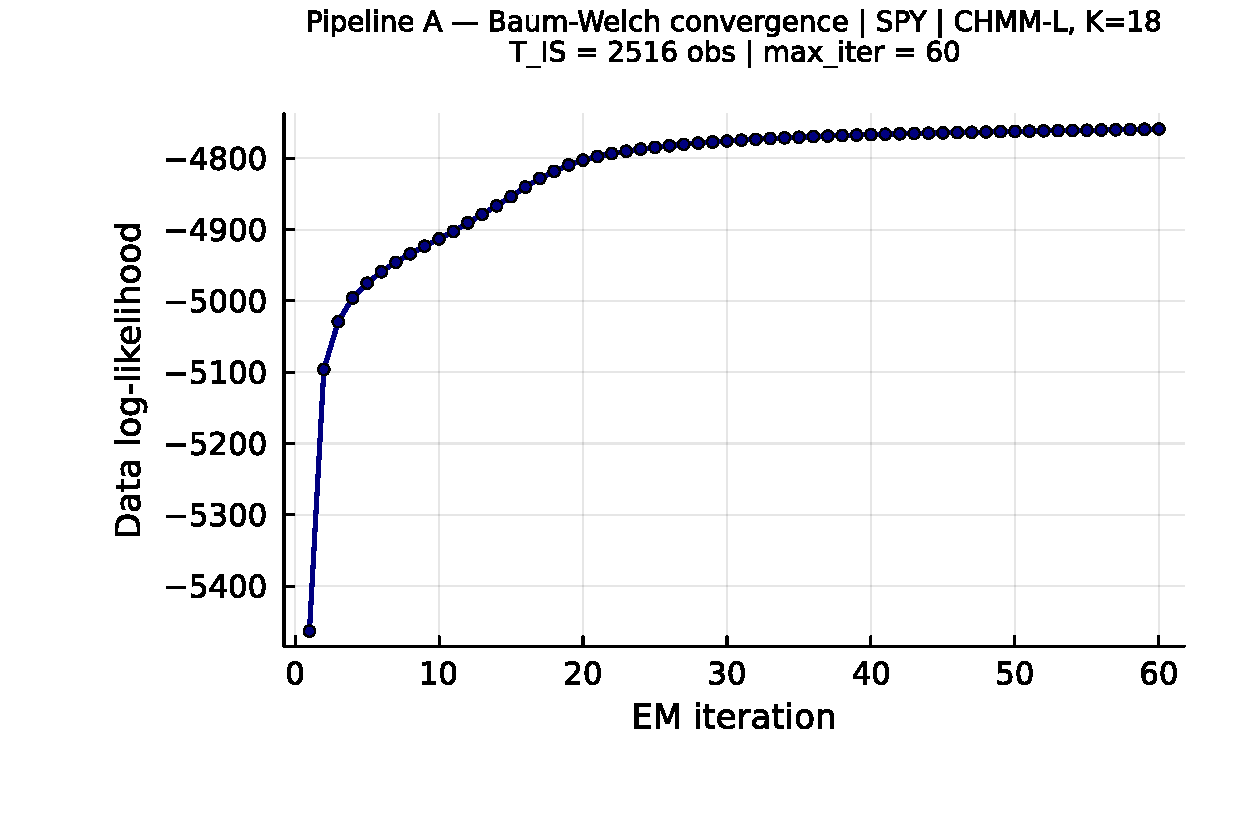
\includegraphics[width=\textwidth]{figs/Fig-Convergence-K18-L.pdf}
    \caption{CHMM-L}
\end{subfigure}
\caption{Log-likelihood histories for the SPY IS fit (Pipeline~A) at $K = 18$ across the three emission families (CHMM-N Gaussian classical EM; CHMM-t Student-t ECM with per-state $\nu_k$ golden-section sub-step; CHMM-L Laplace weighted-EM). All three curves are monotonically non-decreasing and plateau well before the $\texttt{max\_iter} = 60$ budget.}
\label{fig:convergence_families}
\end{figure}

\subsubsection{Ryd\'{e}n K = 2 Replication}
\label{sec:ryden_replication}

Table~\ref{tab:ryden_init} reports the direct replication of Ryd\'{e}n et al.'s 1998 $K = 2$ setting on SPY IS under both initialization strategies, as discussed in Section~\ref{sec:discussion}.
The quantile-based initialization used in the main body is row 1; five independent random-seed initializations are rows 2--6.
Random init here draws per-state $(\mu_k, \sigma_k)$ from a moderate perturbation of the sample moments, which is representative of the random-init practice common in the 1990s HMM literature.

\begin{table}[h]
\centering
\small
\caption{Ryd\'{e}n replication: $K = 2$ CHMM-N on SPY IS under quantile vs random initialization (seed sub-index varies the random init).}
\label{tab:ryden_init}
\begin{tabular}{l c c c c c}
\toprule
Init & KS IS (\%) & AD IS (\%) & ACF-MAE & Kurt IS & KS OoS (\%) \\
\midrule
Quantile (main body) & 79.0 & 71.5 & 0.0501 & 2.57 & 72.4 \\
Random seed = 1      & 78.7 & 70.7 & 0.0502 & 2.57 & 73.2 \\
Random seed = 7      & 75.3 & 69.6 & 0.0498 & 2.56 & 74.0 \\
Random seed = 42     & 77.6 & 70.0 & 0.0498 & 2.59 & 71.8 \\
Random seed = 100    & 76.2 & 69.4 & 0.0500 & 2.59 & 72.3 \\
Random seed = 2024   & 76.4 & 69.8 & 0.0499 & 2.54 & 72.9 \\
\bottomrule
\end{tabular}
\end{table}

The key observation is that ACF-MAE is essentially constant at $\approx 0.050$ across all six rows, matching the $K = 18$ CHMM-N of the main body.
IS KS pass rate remains below the $K = 18$ operating point ($75.3$--$79.0\%$) because two Gaussian components cannot tile the full multi-regime return distribution.
The combination is consistent with the reading that the binding low-$K$ constraint in the \citet{ryden1998stylized} setup is distributional rather than temporal: the ACF is already well reproduced at $K = 2$, and it is distributional fidelity that drives the preference for $K = 18$.



\subsection{Robustness, Test Power, Multi-Seed, and Auxiliary Baselines}
\label{sec:supp_robustness}
\subsection{OoS KS Test-Power Calibration}
\label{sec:ks_power}

Table~\ref{tab:ks_power} reports the two-sample KS test-power calibration used to anchor the OoS KS pass rates of Section~\ref{sec:oos}.
For each of $1{,}000$ Monte Carlo replications (seed = 20260420), a simulated series of length $T_{\text{OoS}} = 572$ is drawn from each of three reference generators and tested against the observed OoS series using the same $\alpha = 0.05$ threshold as the main-body pass-rate metric.

\begin{table}[h]
\centering
\small
\caption{OoS KS pass-rate calibration (1000 replications, seed = 20260420).}
\label{tab:ks_power}
\begin{tabular}{l c}
\toprule
Reference generator & Pass rate (\%) \\
\midrule
I.i.d.\ resamples of $R_{\text{OoS}}$ at length $T_{\text{OoS}} = 572$ (known-correct ceiling) & 100.0 \\
I.i.d.\ resamples of $R_{\text{IS}}$ at length $T_{\text{OoS}} = 572$ (nearly correct)          & 90.0  \\
Gaussian$(\hat\mu_{\text{IS}}, \hat\sigma_{\text{IS}})$ at length $T_{\text{IS}}$ (negative control) & 0.0 \\
\bottomrule
\end{tabular}
\end{table}

The $90.0\%$ "nearly correct" rate is the practical ceiling for the CHMM OoS KS pass rates reported in Section~\ref{sec:oos} ($80$--$84\%$); the $0\%$ rate on the Gaussian misspecified generator confirms that the KS test retains ample power at IS length to reject clearly wrong generators.

\subsection{Walk-Forward Rolling-Window Re-Estimation (Pipeline A)}
\label{sec:walk_forward}

This robustness check lives inside Pipeline A: the CHMM-N is still fit per ticker independently, only the fit window rolls forward. It does not introduce cross-asset coupling, and therefore should not be interpreted alongside the Pipeline B results in Section~\ref{sec:cross_asset}. Table~\ref{tab:walk_forward} reports the quarterly walk-forward re-estimation results referenced in Section~\ref{sec:cross_asset_univariate}.
The walk-forward protocol refits the CHMM-N every $63$ trading days (one quarter) across the $572$-day OoS window, feeding the realized returns of the prior quarter into the training set before each refit.
The rolling protocol recovers a modest $\sim 1$ percentage point on JNJ and a substantial $\sim 15$ percentage points on JPM relative to the fixed-IS baseline, confirming that the stationarity assumption is the principal contributor to the JPM OoS gap while JNJ's OoS gap is already small under the fixed fit.

\begin{table}[h]
\centering
\small
\caption{\textbf{Walk-forward (quarterly CHMM-N refit) vs fixed-IS CHMM-N on JNJ and JPM} (Pipeline A, per-ticker independent fits; walk-forward only rolls the fit window, it does not introduce cross-asset dependence). $K = 18$, 1000 simulated paths per (ticker, mode), seed = 20260420. IS window 2014-01-03 through 2024-01-03; OoS window 2024-01-04 through 2026-04-17 ($T_{\text{OoS}} = 572$). The walk-forward mode refits the CHMM-N every 63 trading days across the OoS window, feeding each completed quarter's realized returns back into the training set before the next refit. Columns report percent KS / AD pass rate at $\alpha = 0.05$, excess kurtosis, ACF-MAE of $|G_t|$, Wasserstein-1, and Hellinger distance.}
\label{tab:walk_forward}
\resizebox{\textwidth}{!}{%
\begin{tabular}{l cc cc cc c c c}
\toprule
Mode & KS IS & AD IS & KS OoS & AD OoS & Kurt IS & Kurt OoS & ACF-MAE & $W_1$ & $H$ \\
\midrule
JNJ fixed-IS      & 99.3 & 98.2 & 94.0 & 92.1 & 5.46 & 4.98 & 0.0322 & 0.095 & 0.0786 \\
JNJ walk-forward  & 99.3 & 98.2 & 94.9 & 91.3 & 5.46 & 5.14 & 0.0322 & 0.095 & 0.0786 \\
JPM fixed-IS      & 96.6 & 94.4 & 49.0 & 48.6 & 7.33 & 6.31 & 0.0449 & 0.165 & 0.0875 \\
JPM walk-forward  & 96.6 & 94.4 & 64.3 & 63.6 & 7.33 & 5.96 & 0.0449 & 0.165 & 0.0875 \\
\bottomrule
\end{tabular}%
}
\end{table}

\subsection{Block-Bootstrap Baseline}
\label{sec:block_bootstrap_supp}

Table~\ref{tab:block_bootstrap} reports the full seven-metric panel for the stationary block bootstrap at block length $b = 10$ trading days, the temporally-aware non-parametric baseline added to Table~\ref{tab:model_comparison}.

\begin{table}[h]
\centering
\small
\caption{Stationary block bootstrap (block length $b = 10$ trading days) on SPY (1000 paths, seed = 20260420).}
\label{tab:block_bootstrap}
\begin{tabular}{l cc cc c c c c}
\toprule
Window & KS & AD & Kurt & ACF-MAE & $W_1$ & $H$ & Cov \\
\midrule
IS  & 99.2 & 96.4 & 7.07 & 0.0568 & 0.092 & 0.0534 & 100.0 \\
OoS & 87.5 & 86.4 & 5.34 & 0.0512 & 0.225 & 0.1570 & 86.9  \\
\bottomrule
\end{tabular}
\end{table}

\subsection{Discrete HMM with Bin-Conditional Student-t Emissions}
\label{sec:bin_t_supp}

Table~\ref{tab:bin_t} reports the full seven-metric panel for the Bin-T NJ variant referenced in Section~\ref{sec:model_comparison}: the discrete NJ transition matrix with $K_{\text{disc}} = 13$ quantile bins, but with each bin emitting from a bin-conditional Student-t density rather than from the bin centroid.

\begin{table}[h]
\centering
\small
\caption{Discrete HMM with bin-conditional Student-t emissions on SPY (no jumps, $K_{\text{disc}} = 13$, 1000 paths, seed = 20260420).}
\label{tab:bin_t}
\begin{tabular}{l cc cc c c c c}
\toprule
Window & KS & AD & Kurt & ACF-MAE & $W_1$ & $H$ & Cov \\
\midrule
IS  & 95.4 & 92.1 & 26.18 & 0.0619 & 0.116 & 0.0929 & 89.9 \\
OoS & 86.7 & 93.2 & 10.76 & 0.0538 & 0.177 & 0.1614 & 93.9 \\
\bottomrule
\end{tabular}
\end{table}

The bin-conditional Student-t fit picks $\nu \approx 2.71$ for the two extreme bins (bins $1$ and $13$, corresponding to the lower and upper quantile tails of the IS distribution) and $\nu = 50$ (upper bracket) for the eleven central bins, which explains both the large in-sample simulated kurtosis ($26.18$) and the very thin-scale central bins ($\sigma$ $\sim$ $0.06$--$0.28$).



\subsection{GRU Deep-Generative Baseline}
\label{sec:gru_supp}

Architecture and training details for the GRU baseline used in
Section~\ref{sec:model_comparison} are summarised here.

\begin{itemize}
    \item \textbf{Architecture.} A single-layer Gated Recurrent Unit (GRU)
    with hidden dimension $H = 32$ followed by a Dense head with two
    outputs $(\mu_t, \log \sigma_t)$. Input is a single feature (the
    standardised return) over a context window of $w = 20$ trading days.

    \item \textbf{Loss.} Per-window negative log-likelihood of a Gaussian
    next-step density, equation~\eqref{eq:gru_nll}.

    \item \textbf{Optimiser.} Adam, learning rate $1.0 \times 10^{-3}$.

    \item \textbf{Training schedule.} $20$ epochs, full pass per epoch
    over $T_{\text{IS}} - w$ training windows, randomly shuffled at each
    epoch.

    \item \textbf{Numerical stability.} $\log \sigma_t$ is clamped to
    $[-6, 4]$ inside the loss to prevent gradient explosion when the
    network attempts to assign vanishingly-small variance to extreme
    observations.

    \item \textbf{Pre-processing.} The input return series is standardised
    by its in-sample mean and standard deviation; predictions are
    re-scaled back at sampling time.

    \item \textbf{Synthesis.} The trailing $w$ in-sample returns seed the
    recurrence; for each generation step the predicted Gaussian is
    sampled, the sample is appended to the context window, and the
    procedure rolls forward. The first $64$ steps are discarded as
    burn-in.

    \item \textbf{Implementation.} Julia using \texttt{Flux.jl}
    \cite{innes2018flux} with the \texttt{Optimisers.Adam} state.
    Random seed for weight initialisation, training shuffling, and per-path
    sampling: $20260420$, with deterministic per-path sub-seeds.
\end{itemize}

The trained model is callable through the same
\texttt{simulate\_gru(model, n\_steps; seed\_window)} interface as the
CHMM and discrete-HMM models, so the seven-metric panel evaluates the GRU
on byte-identical windows to the other generators.

\begin{table}[h]
\centering
\small
\caption{GRU deep-generative baseline on SPY (single-layer, hidden $H=32$, window $w=20$, $20$ epochs, Adam $\eta=10^{-3}$, $1{,}000$ paths, seed = 20260420). Final training NLL: $0.2005$.}
\label{tab:gru}
\begin{tabular}{l cc c c c c c}
\toprule
Window & KS & AD & Kurt & ACF-MAE & $W_1$ & $H$ & Cov \\
\midrule
IS  & 18.1 & 13.7 & 2.85 & 0.0518 & 0.196 & 0.0966 & 37.4 \\
OoS & 52.5 & 55.0 & 2.21 & 0.0500 & 0.293 & 0.1603 & 69.7 \\
\bottomrule
\end{tabular}
\end{table}

\subsection{Per-Ticker OoS Price-Simulation Figures (Unconditional CHMM)}
\label{sec:price_sim_oos_appendix}

This appendix collects the per-ticker price-fan and terminal-distribution figures deferred from Section~\ref{sec:price_sim_oos} for the four non-body tickers JNJ, JPM, AAPL, and QQQ.
All figures use the same plotting conventions as Figure~\ref{fig:price_fan_spy} in the main body: blue shaded bands are the $5$--$95\%$ and $25$--$75\%$ quantile envelopes of the $500$ simulated paths, blue solid line is the simulated median, red solid line is the observed OoS price track.
Terminal histograms follow the conventions of Figure~\ref{fig:price_terminal_hists}.
Summary metrics for all four tickers are in Tables~\ref{tab:price_sim_oos} and~\ref{tab:price_sim_path_metrics} in the main body.

\begin{figure}[h]
\centering
\begin{subfigure}[t]{0.32\textwidth}
    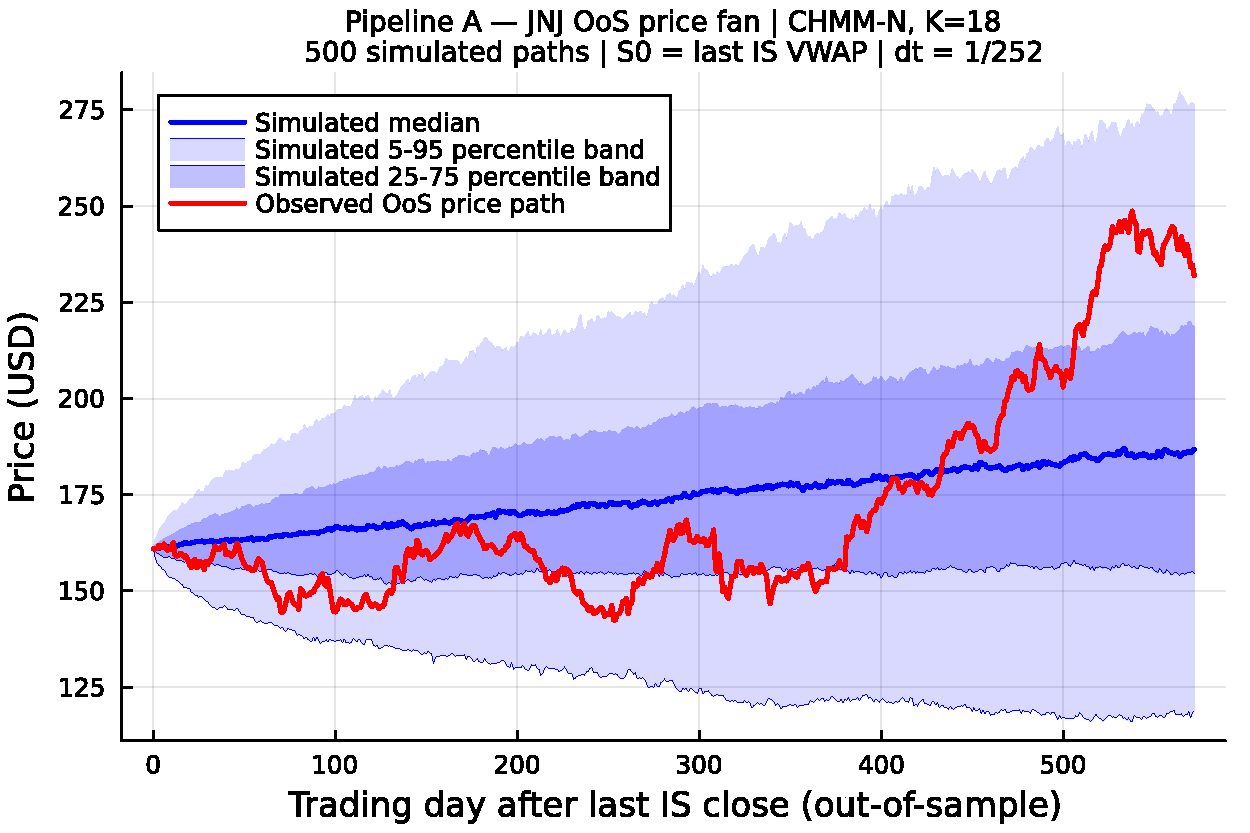
\includegraphics[width=\textwidth]{figs/Fig-JNJ-PriceFan-N.pdf}
    \caption{CHMM-N.}
\end{subfigure}
\begin{subfigure}[t]{0.32\textwidth}
    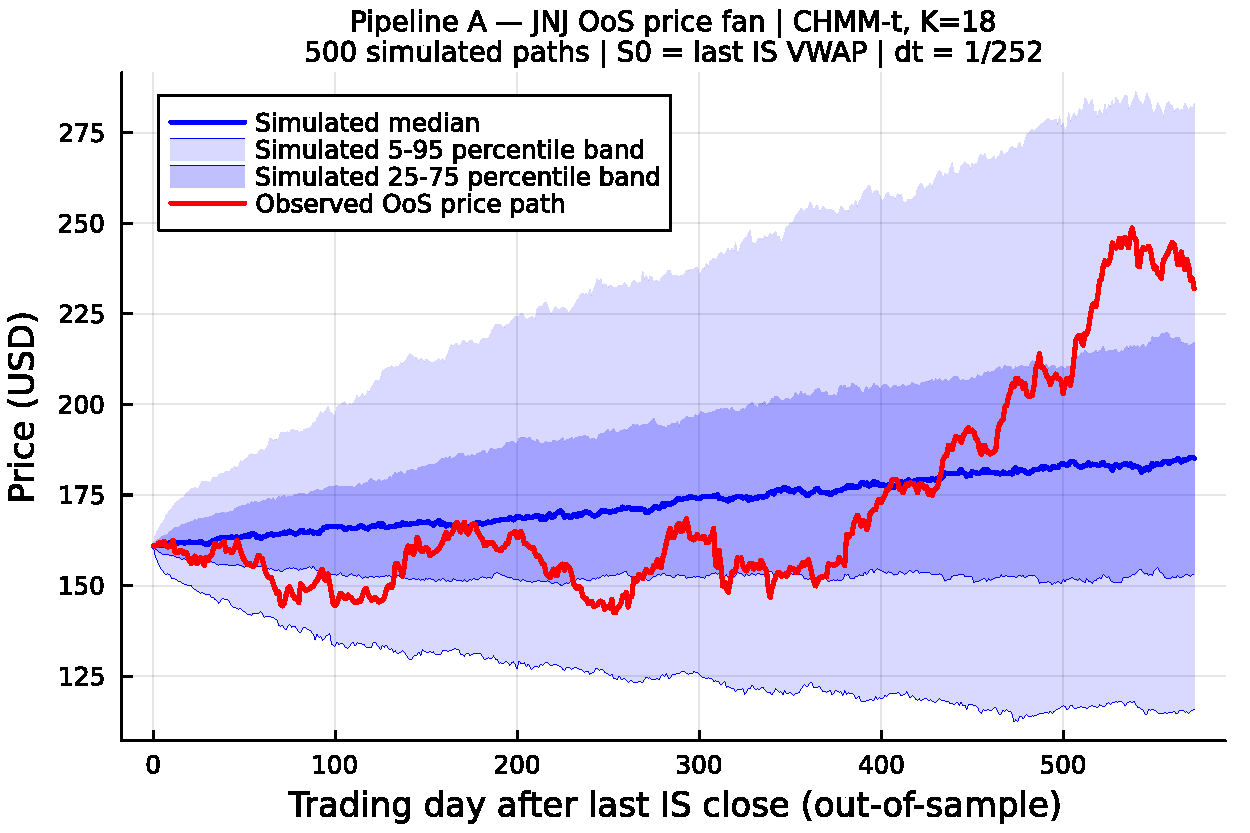
\includegraphics[width=\textwidth]{figs/Fig-JNJ-PriceFan-t.pdf}
    \caption{CHMM-t.}
\end{subfigure}
\begin{subfigure}[t]{0.32\textwidth}
    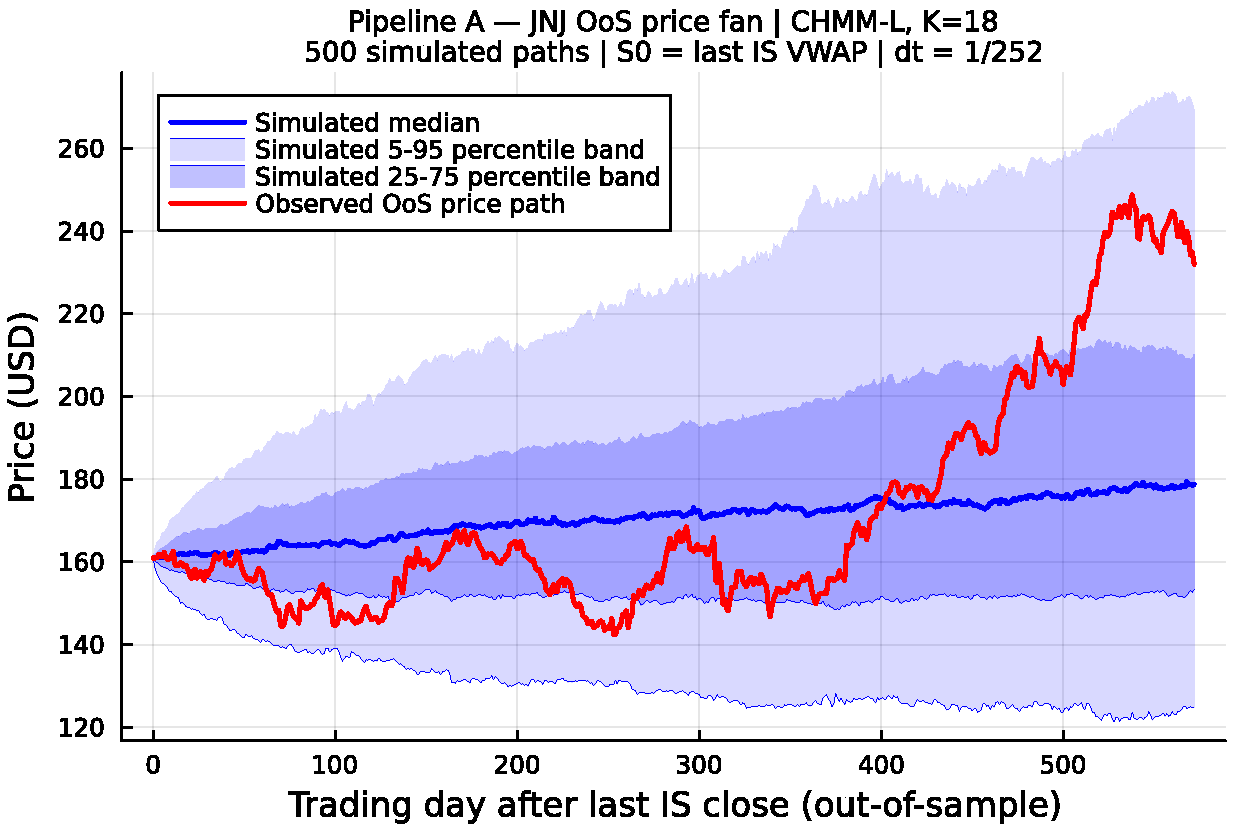
\includegraphics[width=\textwidth]{figs/Fig-JNJ-PriceFan-L.pdf}
    \caption{CHMM-L.}
\end{subfigure}
\caption{JNJ out-of-sample price fan, unconditional CHMM sampler.}
\label{fig:price_fan_jnj_appendix}
\end{figure}

\begin{figure}[h]
\centering
\begin{subfigure}[t]{0.32\textwidth}
    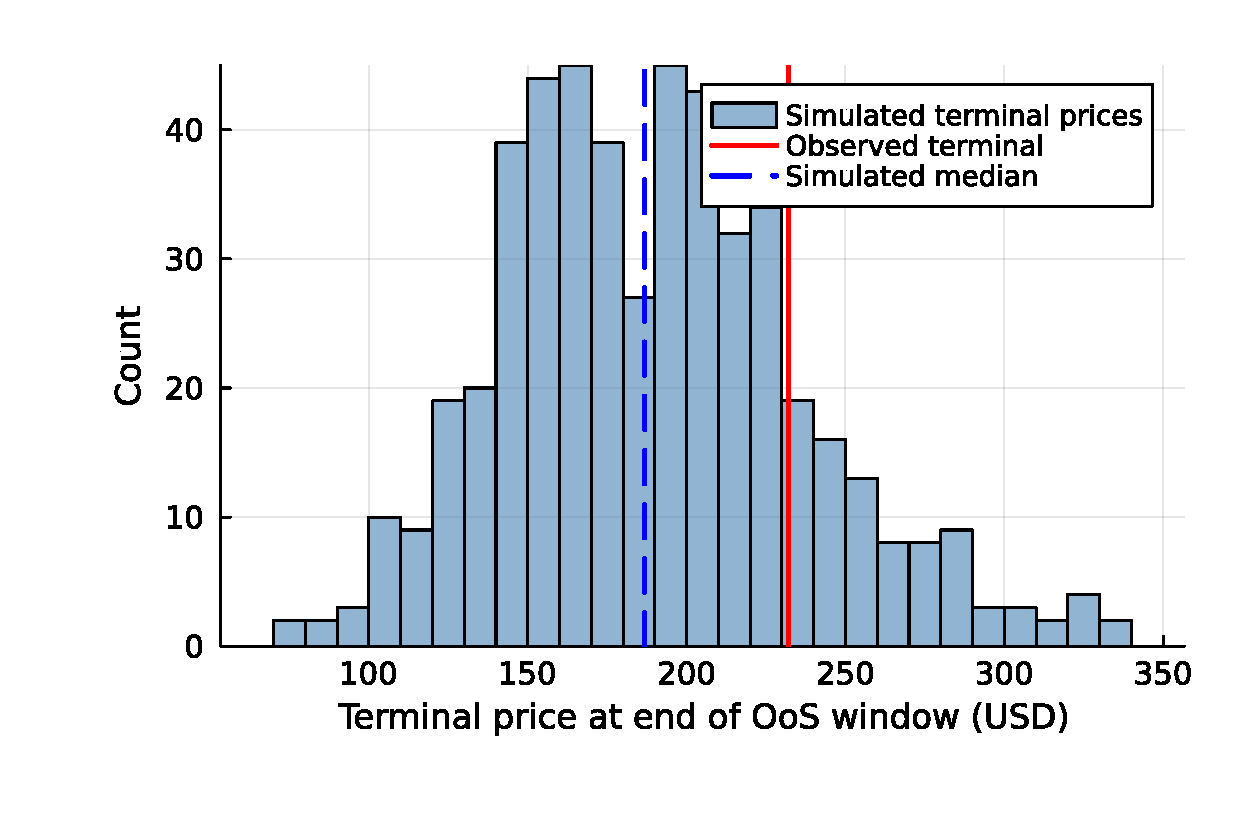
\includegraphics[width=\textwidth]{figs/Fig-JNJ-TerminalDist-N.pdf}
    \caption{CHMM-N.}
\end{subfigure}
\begin{subfigure}[t]{0.32\textwidth}
    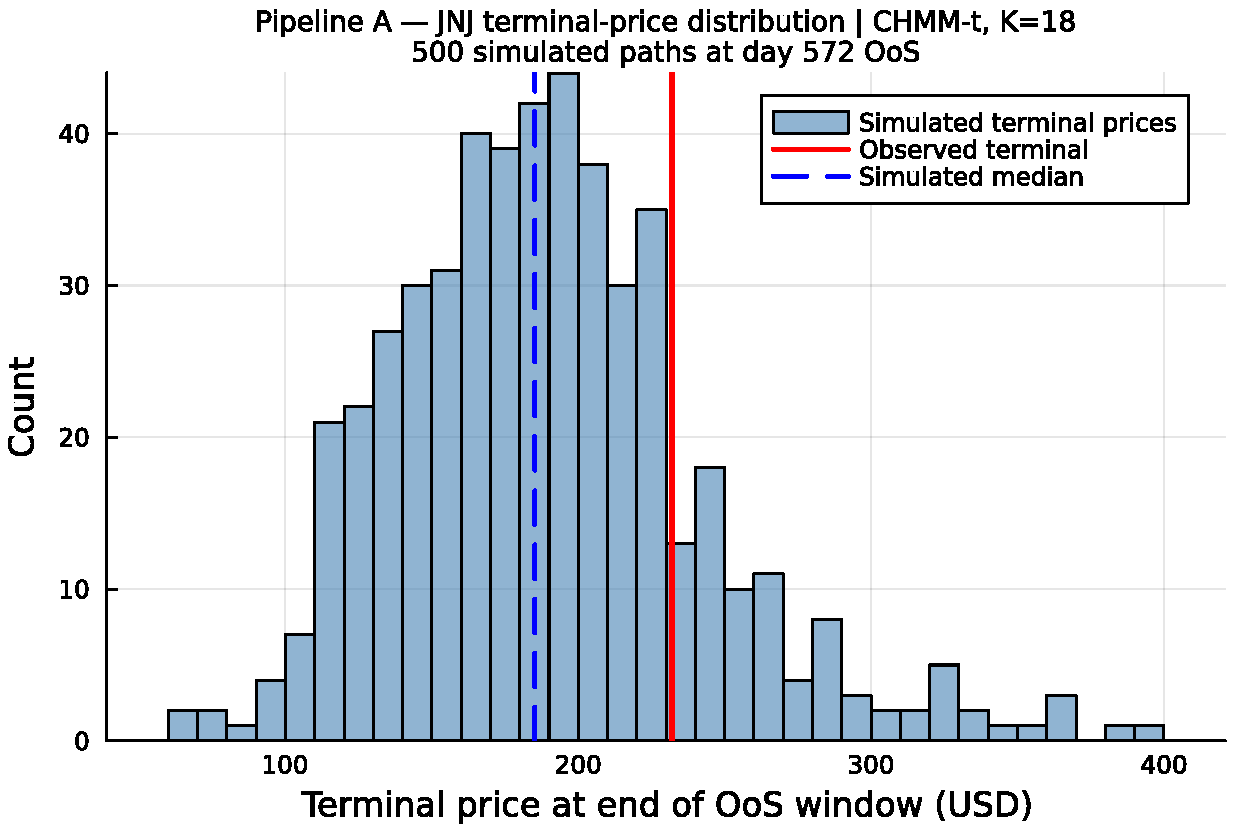
\includegraphics[width=\textwidth]{figs/Fig-JNJ-TerminalDist-t.pdf}
    \caption{CHMM-t.}
\end{subfigure}
\begin{subfigure}[t]{0.32\textwidth}
    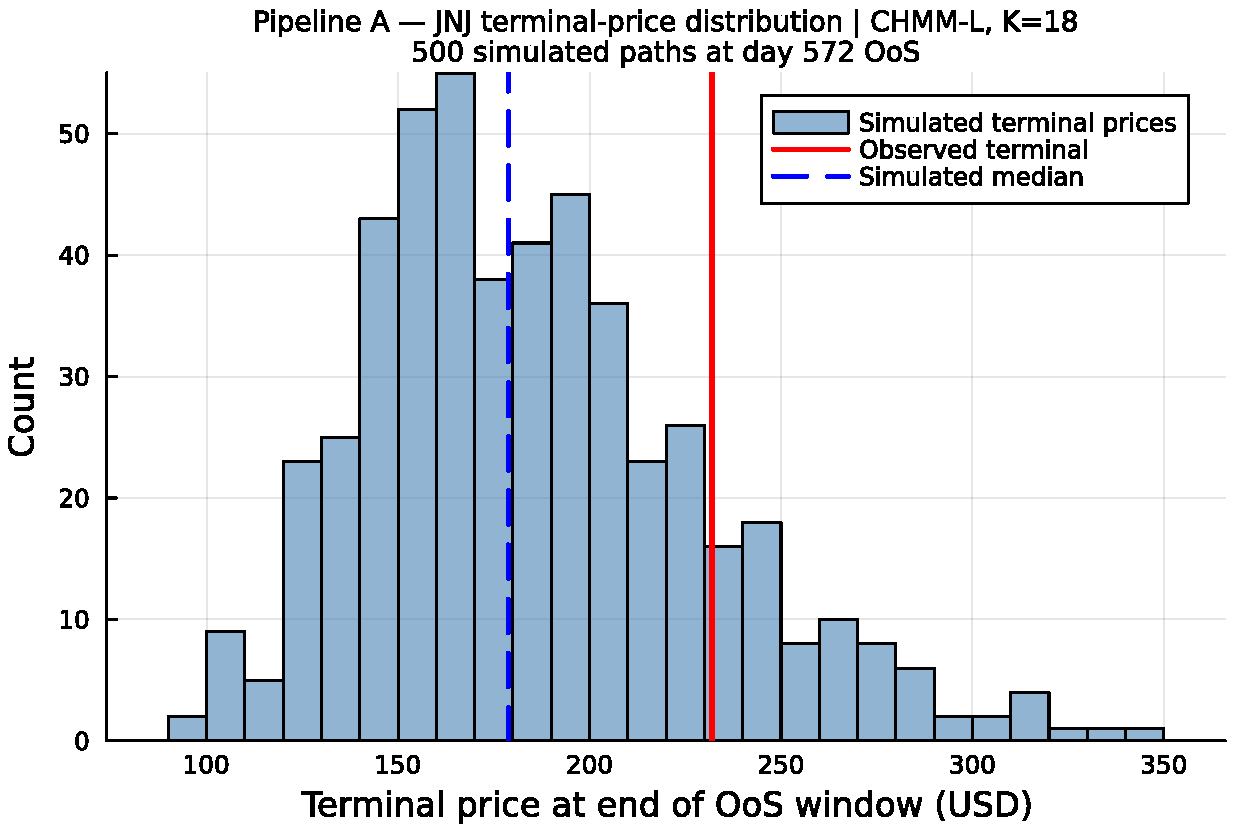
\includegraphics[width=\textwidth]{figs/Fig-JNJ-TerminalDist-L.pdf}
    \caption{CHMM-L.}
\end{subfigure}
\caption{JNJ terminal-price distribution, unconditional CHMM sampler.}
\label{fig:terminal_jnj_appendix}
\end{figure}

\begin{figure}[h]
\centering
\begin{subfigure}[t]{0.32\textwidth}
    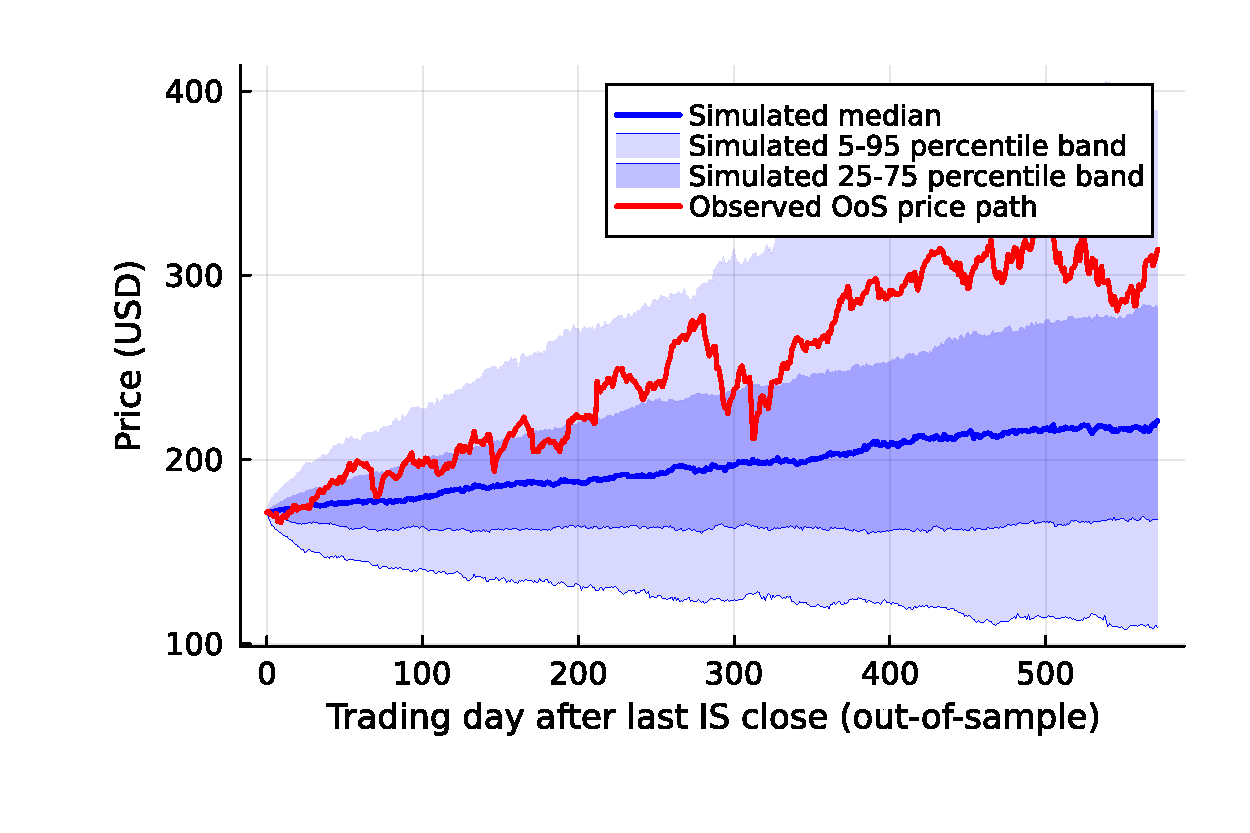
\includegraphics[width=\textwidth]{figs/Fig-JPM-PriceFan-N.pdf}
    \caption{CHMM-N.}
\end{subfigure}
\begin{subfigure}[t]{0.32\textwidth}
    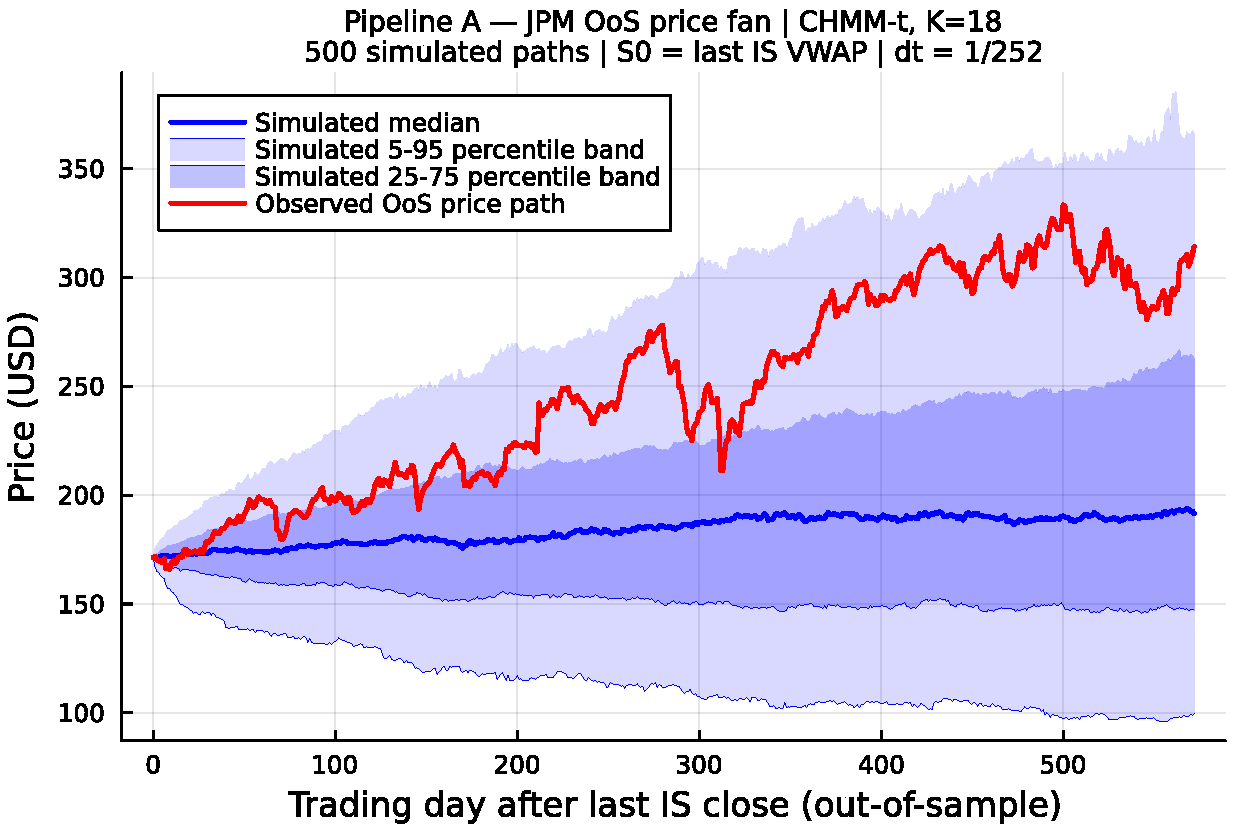
\includegraphics[width=\textwidth]{figs/Fig-JPM-PriceFan-t.pdf}
    \caption{CHMM-t.}
\end{subfigure}
\begin{subfigure}[t]{0.32\textwidth}
    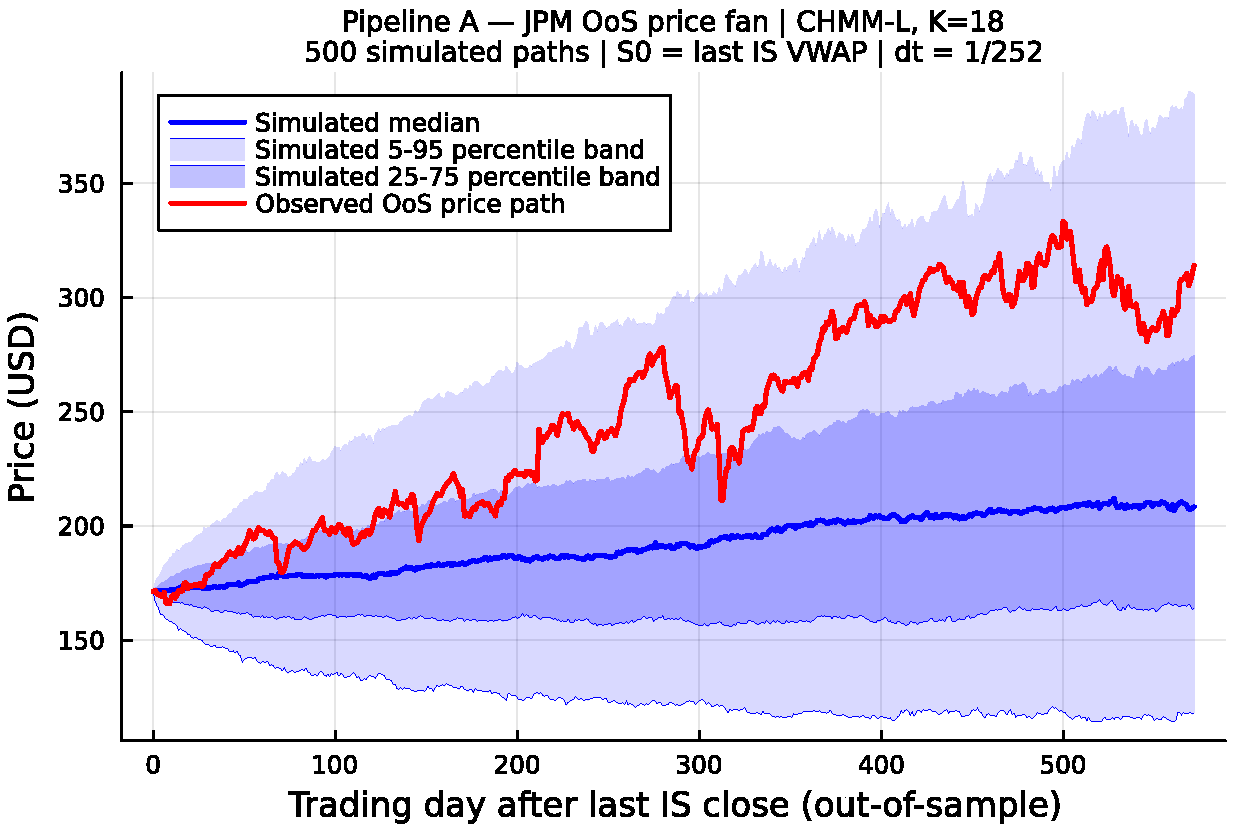
\includegraphics[width=\textwidth]{figs/Fig-JPM-PriceFan-L.pdf}
    \caption{CHMM-L.}
\end{subfigure}
\caption{JPM out-of-sample price fan, unconditional CHMM sampler.}
\label{fig:price_fan_jpm_appendix}
\end{figure}

\begin{figure}[h]
\centering
\begin{subfigure}[t]{0.32\textwidth}
    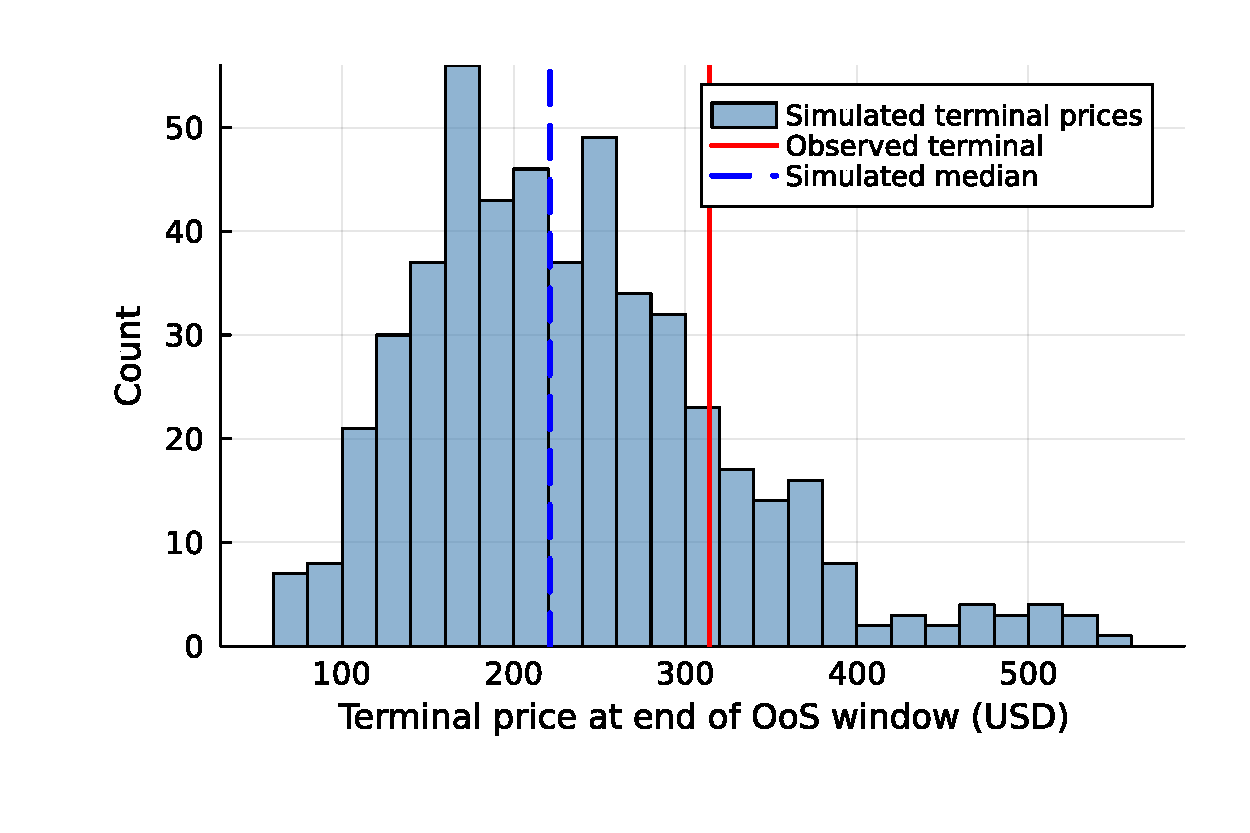
\includegraphics[width=\textwidth]{figs/Fig-JPM-TerminalDist-N.pdf}
    \caption{CHMM-N.}
\end{subfigure}
\begin{subfigure}[t]{0.32\textwidth}
    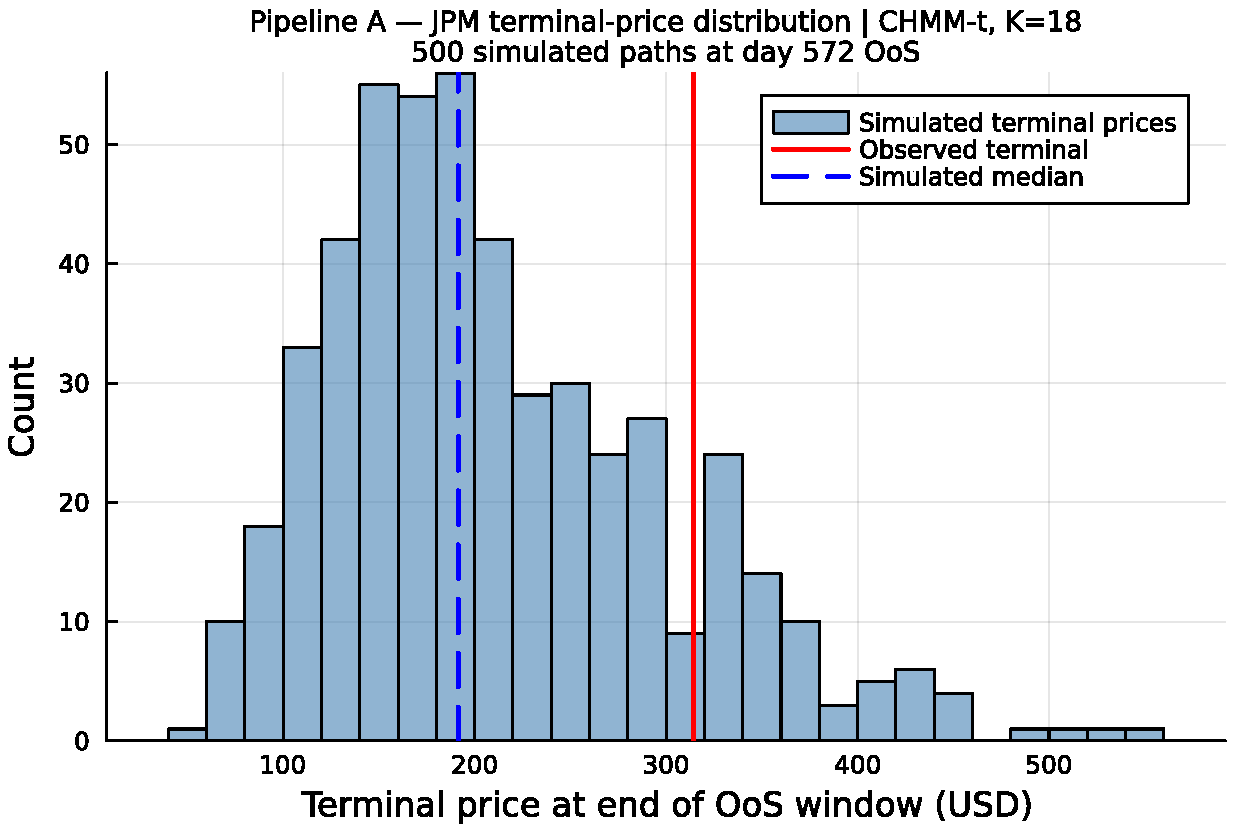
\includegraphics[width=\textwidth]{figs/Fig-JPM-TerminalDist-t.pdf}
    \caption{CHMM-t.}
\end{subfigure}
\begin{subfigure}[t]{0.32\textwidth}
    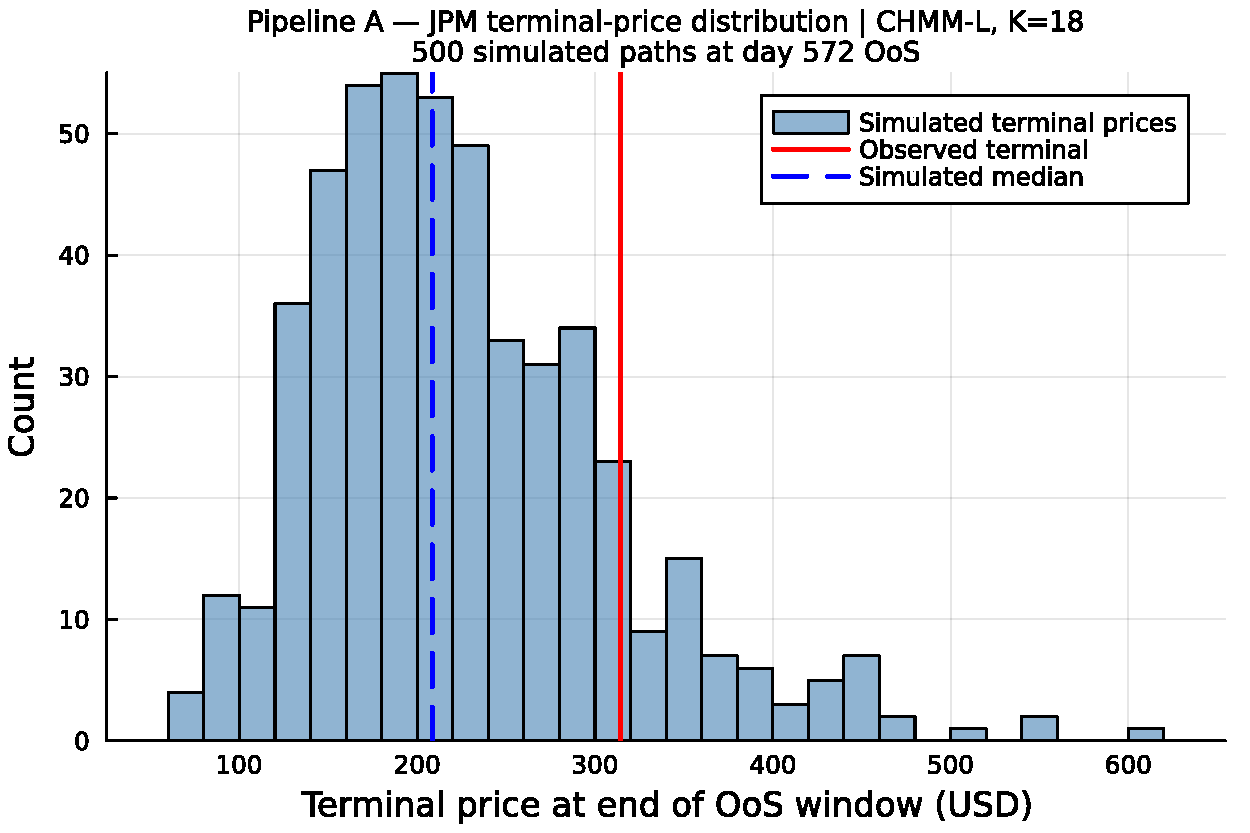
\includegraphics[width=\textwidth]{figs/Fig-JPM-TerminalDist-L.pdf}
    \caption{CHMM-L.}
\end{subfigure}
\caption{JPM terminal-price distribution, unconditional CHMM sampler.}
\label{fig:terminal_jpm_appendix}
\end{figure}

\begin{figure}[h]
\centering
\begin{subfigure}[t]{0.32\textwidth}
    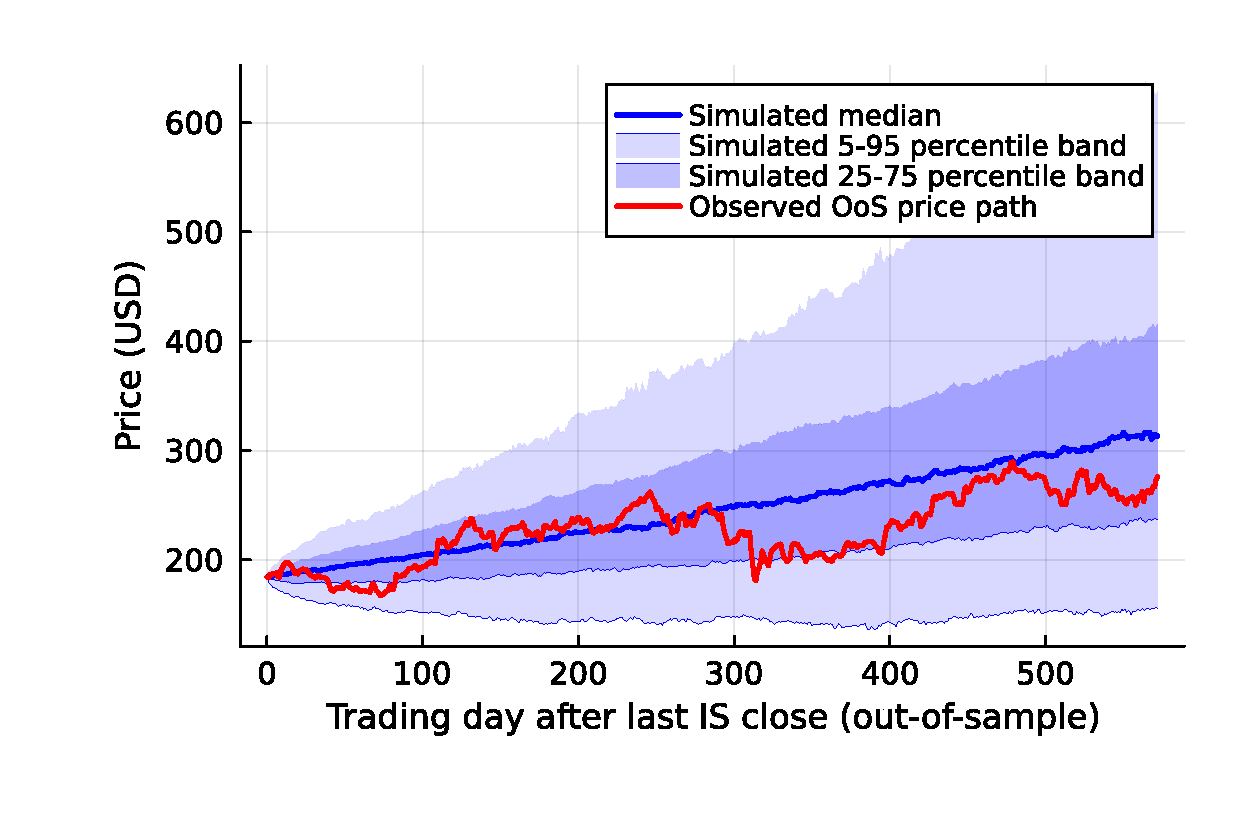
\includegraphics[width=\textwidth]{figs/Fig-AAPL-PriceFan-N.pdf}
    \caption{CHMM-N.}
\end{subfigure}
\begin{subfigure}[t]{0.32\textwidth}
    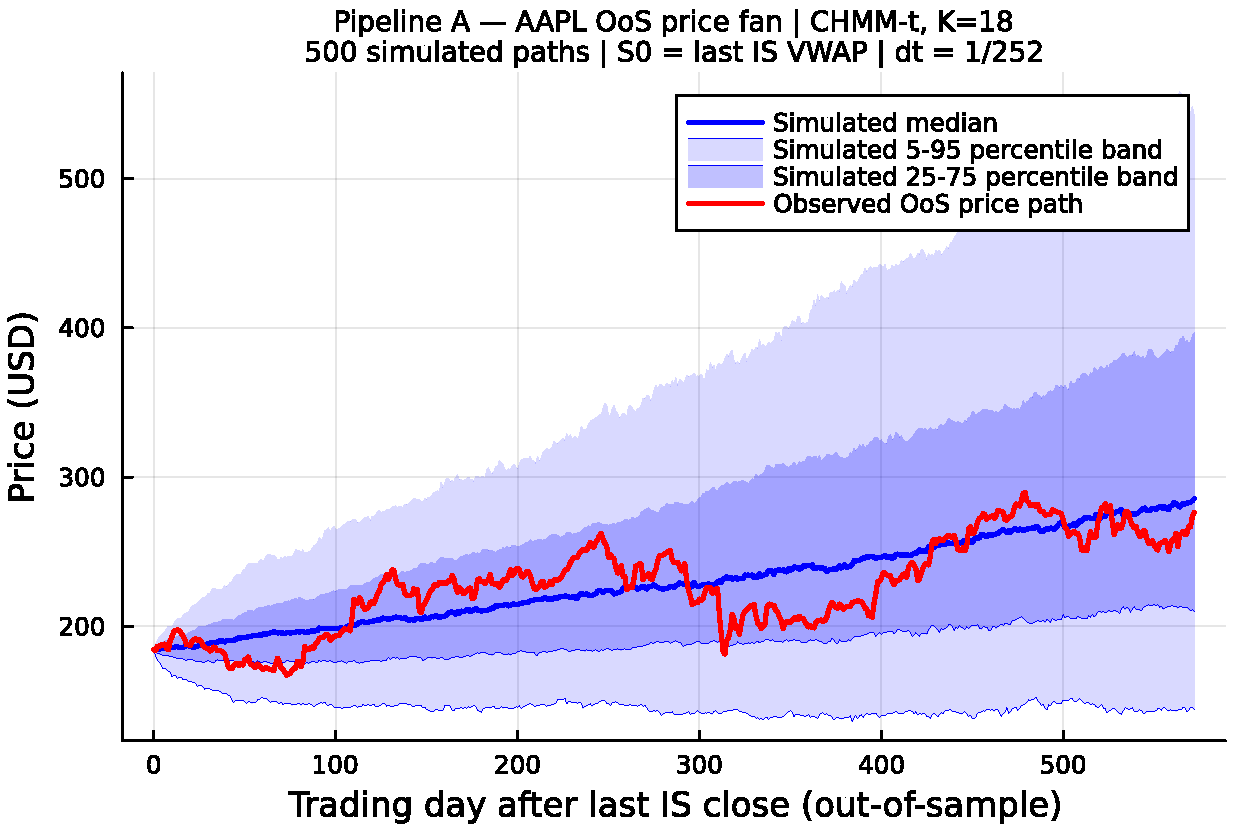
\includegraphics[width=\textwidth]{figs/Fig-AAPL-PriceFan-t.pdf}
    \caption{CHMM-t.}
\end{subfigure}
\begin{subfigure}[t]{0.32\textwidth}
    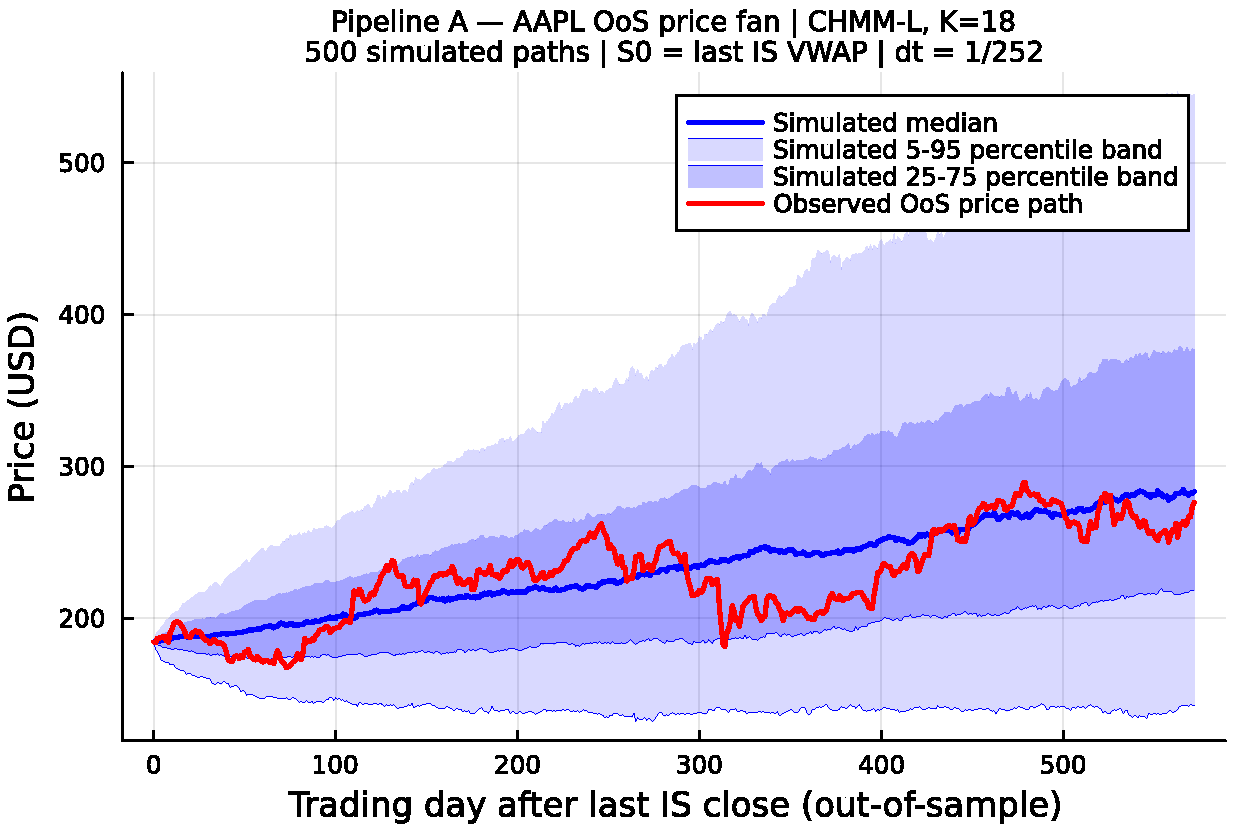
\includegraphics[width=\textwidth]{figs/Fig-AAPL-PriceFan-L.pdf}
    \caption{CHMM-L.}
\end{subfigure}
\caption{AAPL out-of-sample price fan, unconditional CHMM sampler.}
\label{fig:price_fan_aapl_appendix}
\end{figure}

\begin{figure}[h]
\centering
\begin{subfigure}[t]{0.32\textwidth}
    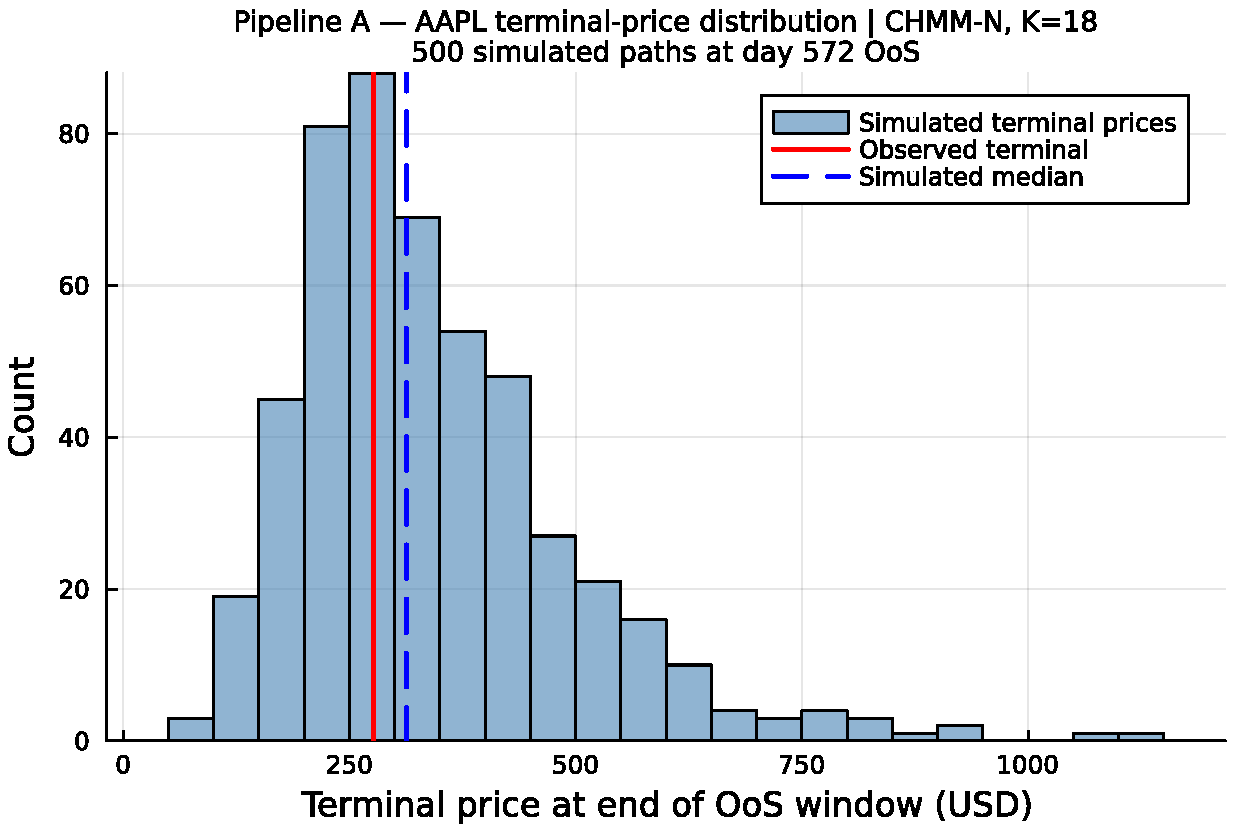
\includegraphics[width=\textwidth]{figs/Fig-AAPL-TerminalDist-N.pdf}
    \caption{CHMM-N.}
\end{subfigure}
\begin{subfigure}[t]{0.32\textwidth}
    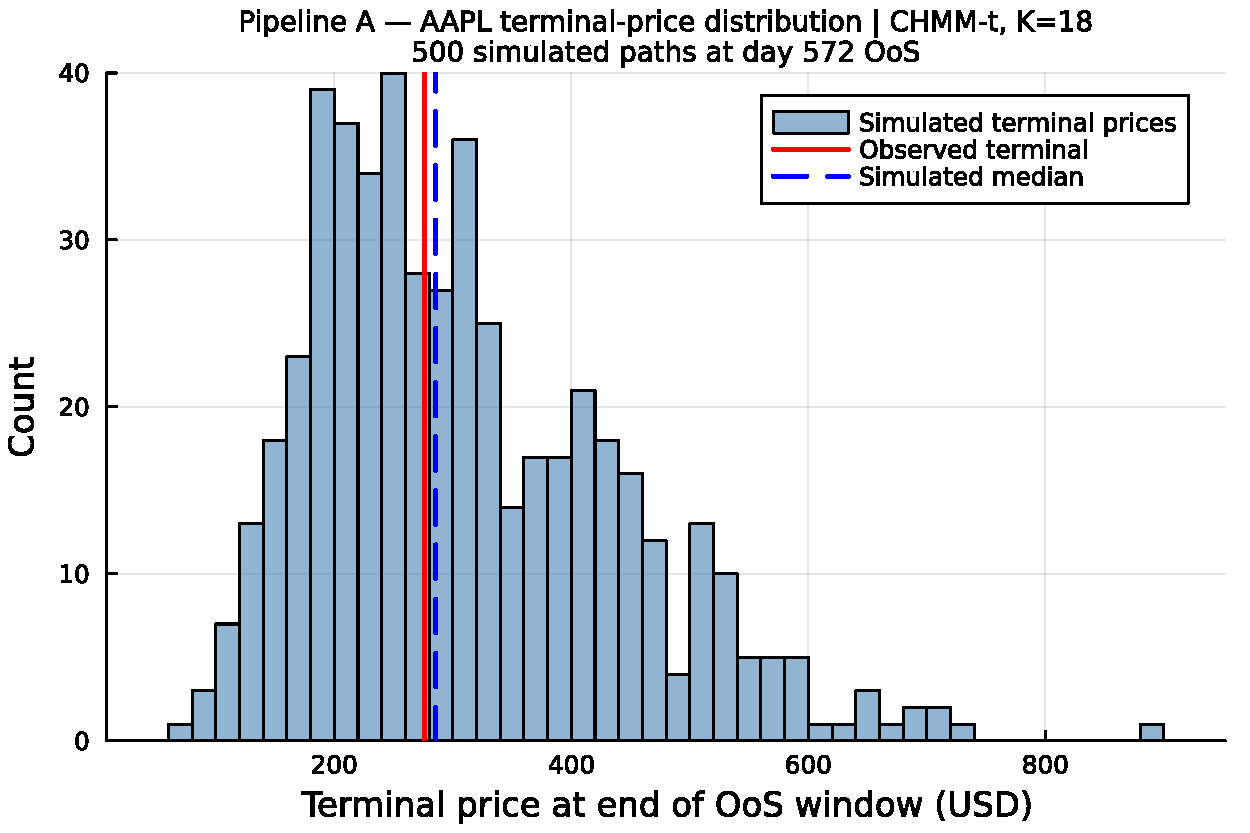
\includegraphics[width=\textwidth]{figs/Fig-AAPL-TerminalDist-t.pdf}
    \caption{CHMM-t.}
\end{subfigure}
\begin{subfigure}[t]{0.32\textwidth}
    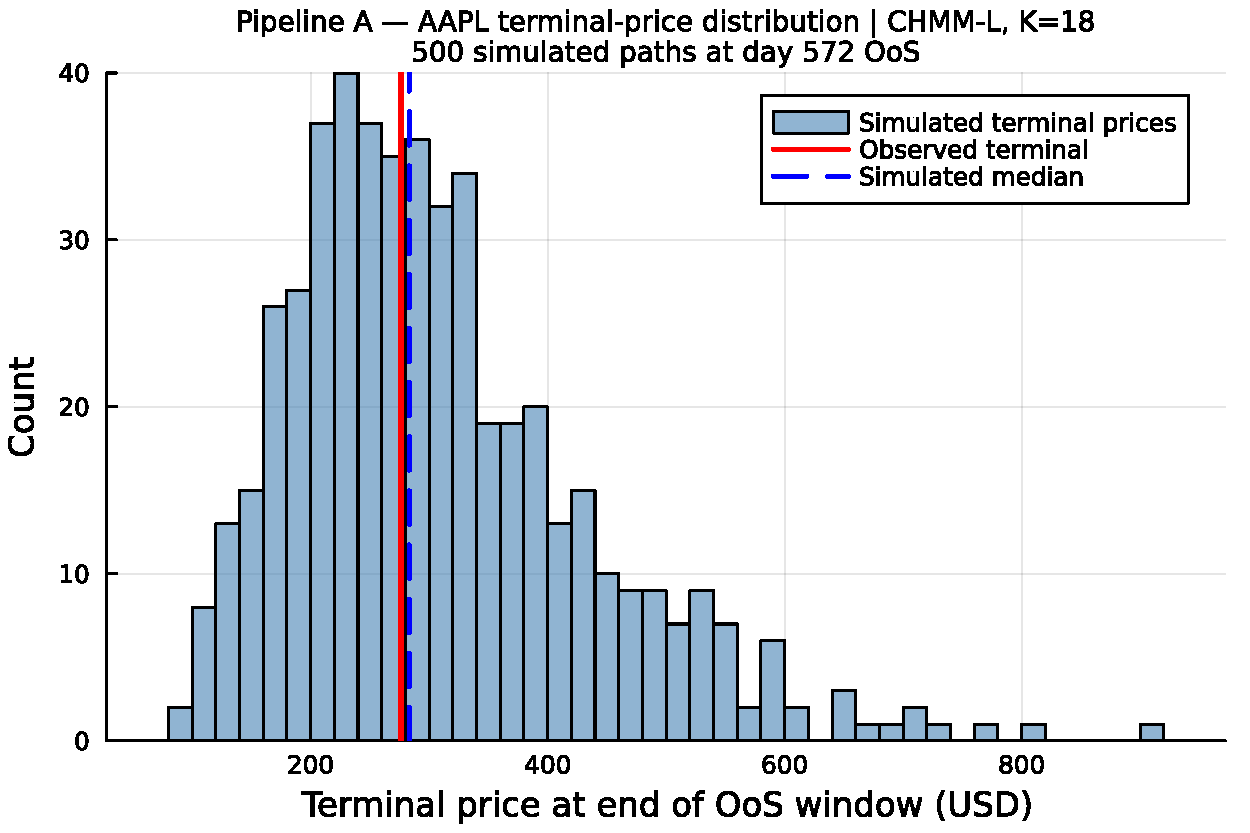
\includegraphics[width=\textwidth]{figs/Fig-AAPL-TerminalDist-L.pdf}
    \caption{CHMM-L.}
\end{subfigure}
\caption{AAPL terminal-price distribution, unconditional CHMM sampler.}
\label{fig:terminal_aapl_appendix}
\end{figure}

\begin{figure}[h]
\centering
\begin{subfigure}[t]{0.32\textwidth}
    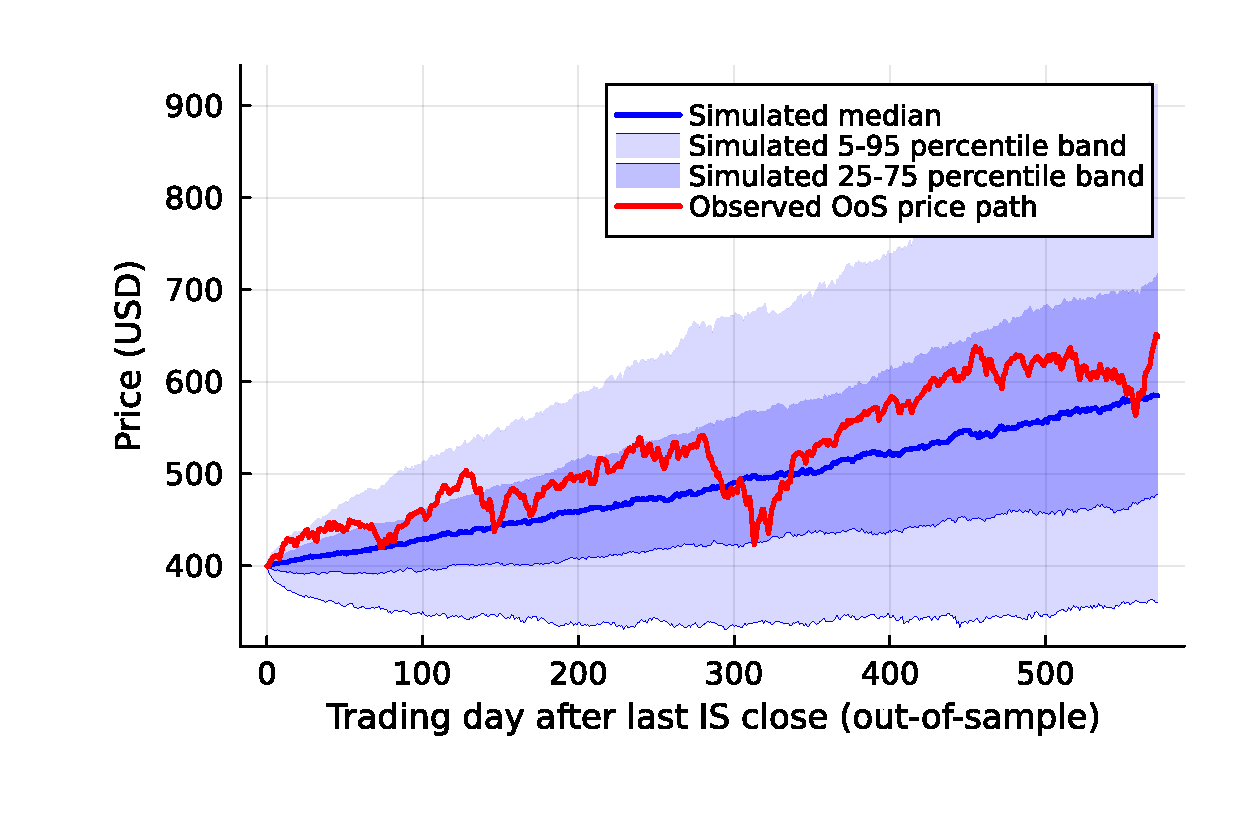
\includegraphics[width=\textwidth]{figs/Fig-QQQ-PriceFan-N.pdf}
    \caption{CHMM-N.}
\end{subfigure}
\begin{subfigure}[t]{0.32\textwidth}
    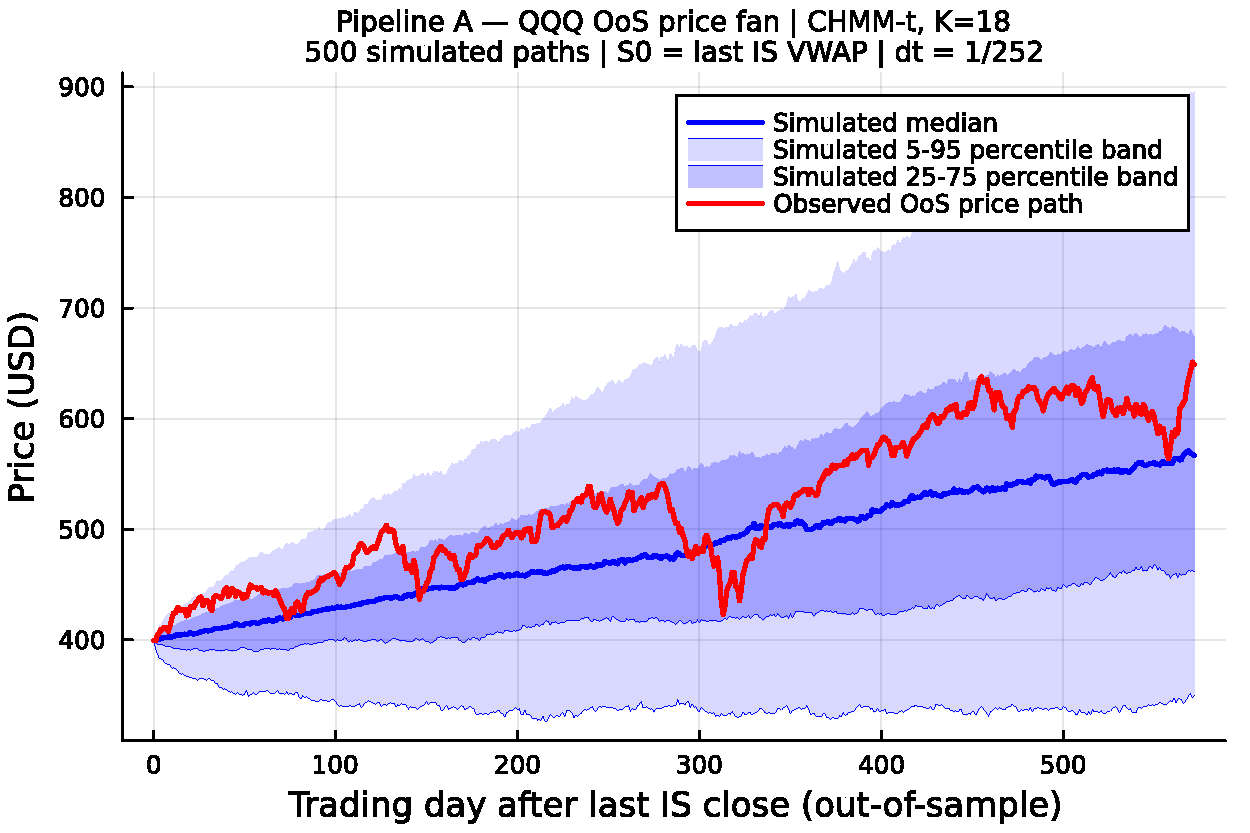
\includegraphics[width=\textwidth]{figs/Fig-QQQ-PriceFan-t.pdf}
    \caption{CHMM-t.}
\end{subfigure}
\begin{subfigure}[t]{0.32\textwidth}
    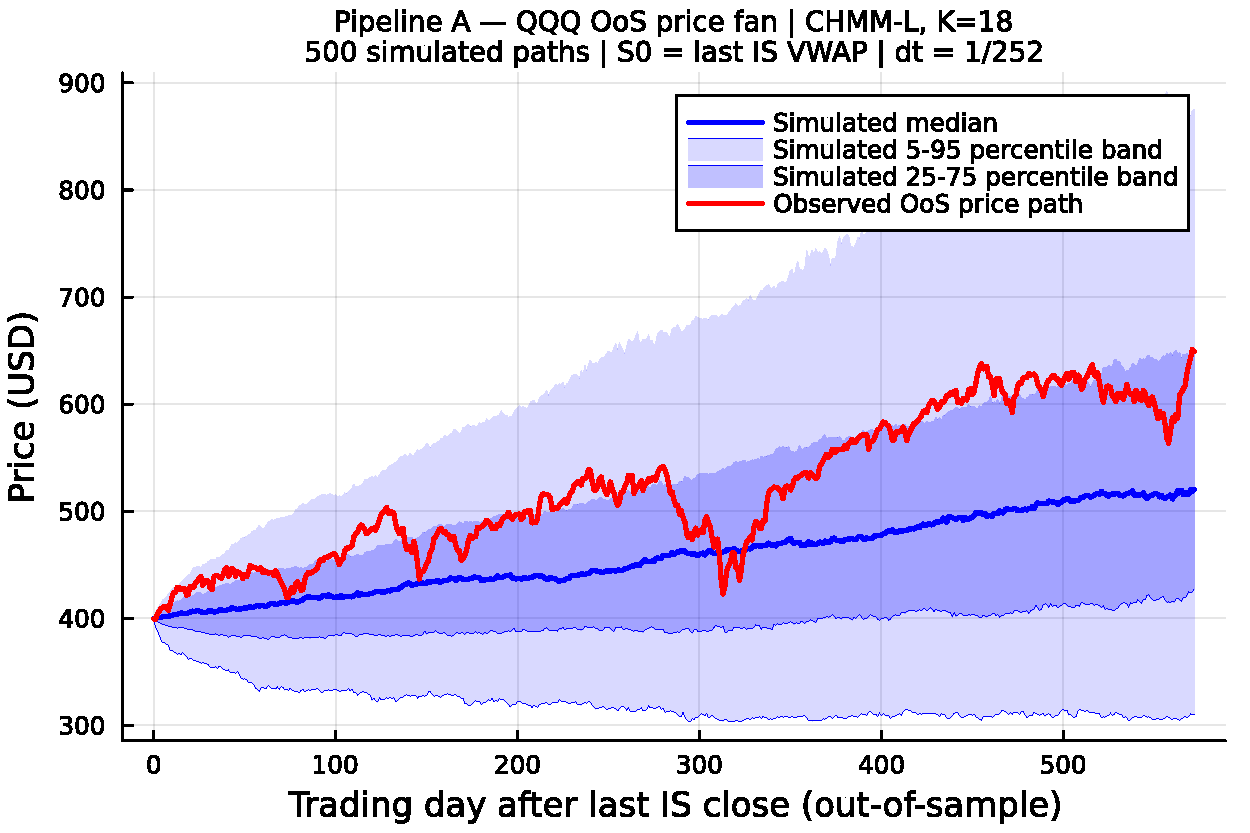
\includegraphics[width=\textwidth]{figs/Fig-QQQ-PriceFan-L.pdf}
    \caption{CHMM-L.}
\end{subfigure}
\caption{QQQ out-of-sample price fan, unconditional CHMM sampler.}
\label{fig:price_fan_qqq_appendix}
\end{figure}

\begin{figure}[h]
\centering
\begin{subfigure}[t]{0.32\textwidth}
    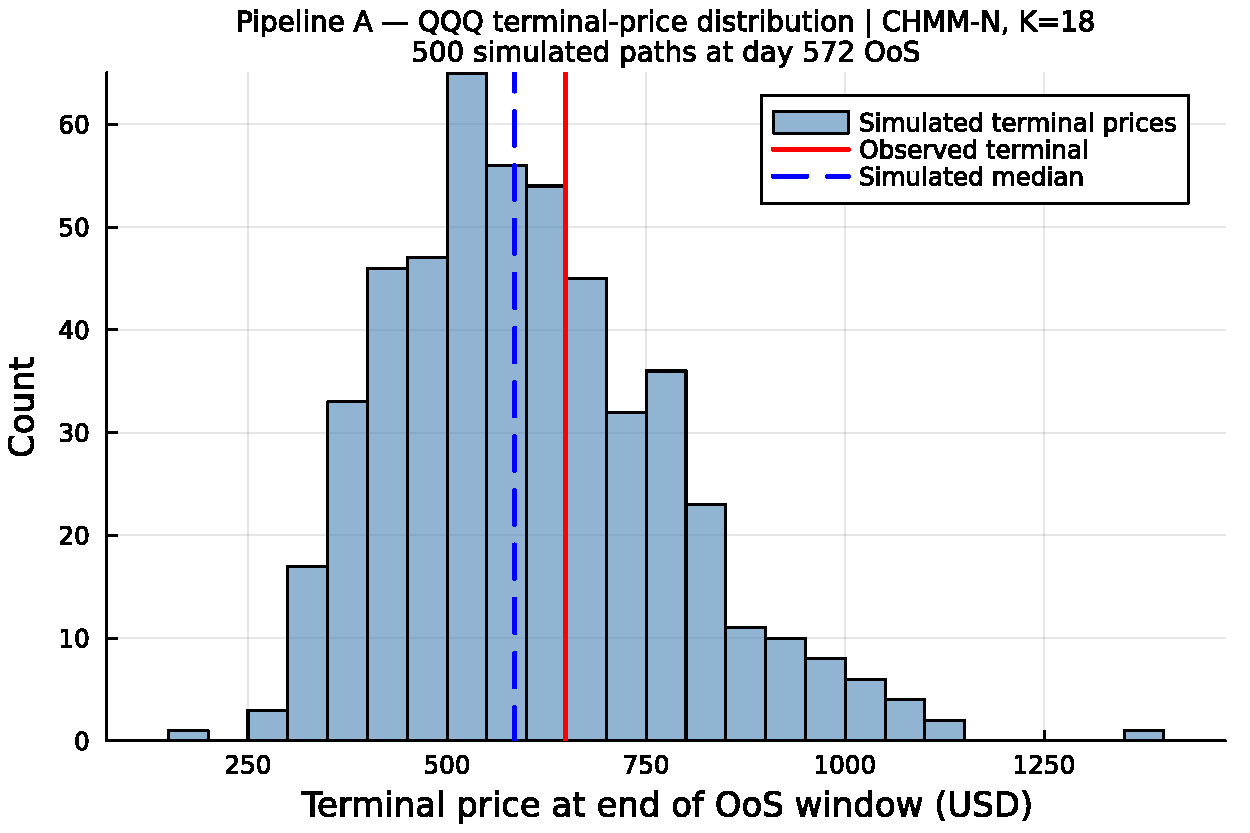
\includegraphics[width=\textwidth]{figs/Fig-QQQ-TerminalDist-N.pdf}
    \caption{CHMM-N.}
\end{subfigure}
\begin{subfigure}[t]{0.32\textwidth}
    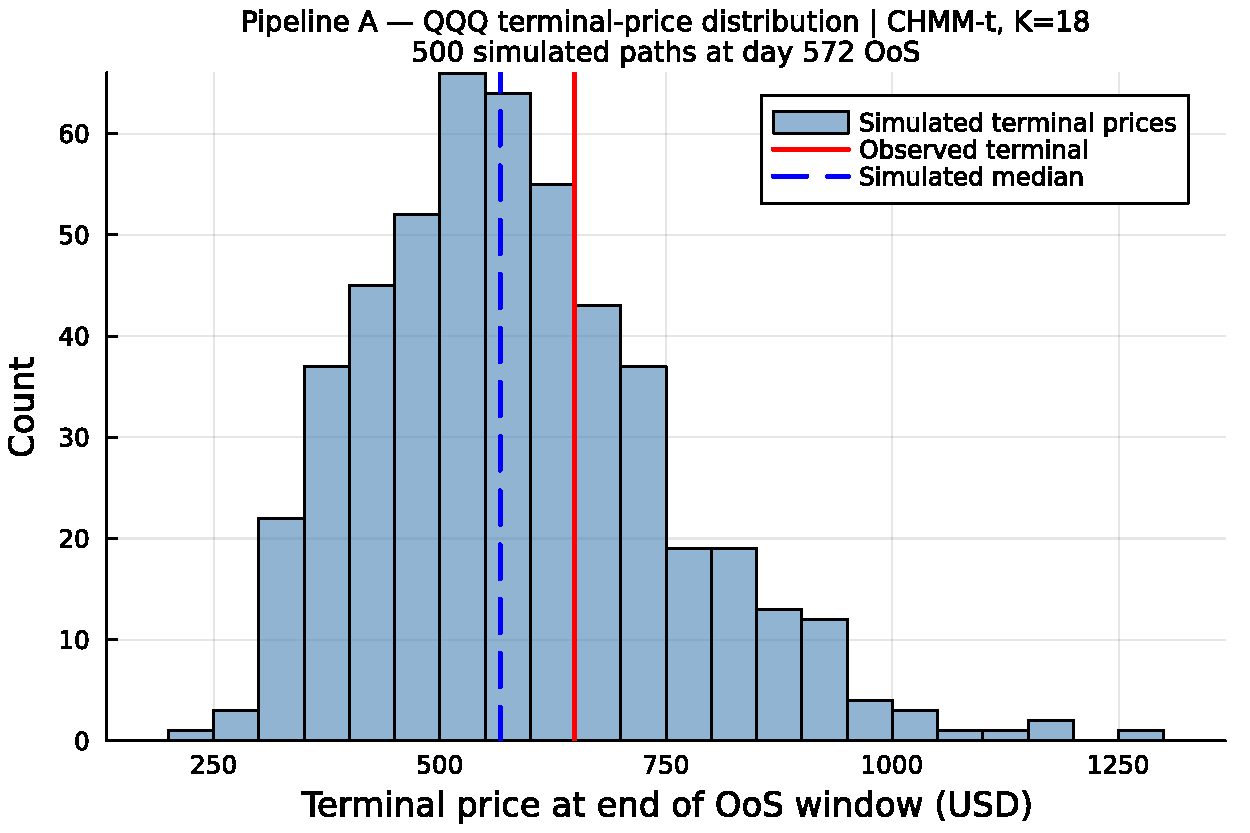
\includegraphics[width=\textwidth]{figs/Fig-QQQ-TerminalDist-t.pdf}
    \caption{CHMM-t.}
\end{subfigure}
\begin{subfigure}[t]{0.32\textwidth}
    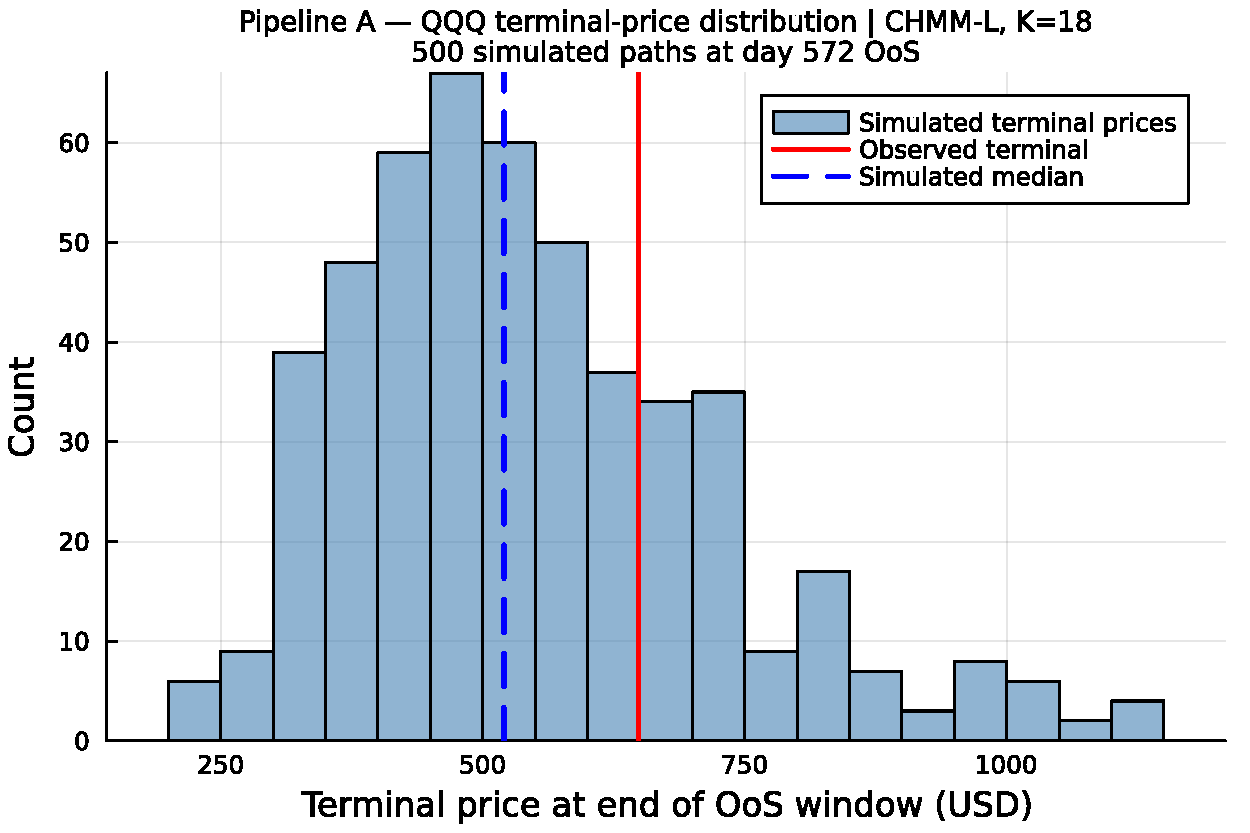
\includegraphics[width=\textwidth]{figs/Fig-QQQ-TerminalDist-L.pdf}
    \caption{CHMM-L.}
\end{subfigure}
\caption{QQQ terminal-price distribution, unconditional CHMM sampler.}
\label{fig:terminal_qqq_appendix}
\end{figure}




\subsection{Cross-Asset Dependence: Full Pipeline~B Panel}
\label{sec:supp_cross_asset}
\subsubsection{Cross-Asset Dependence Models: Derivations and Diagnostics (Pipeline~B)}
\label{sec:cross_asset_supp}

This appendix provides the technical background for the SIM and copula constructions used in Section~\ref{sec:cross_asset} of the main text. These constructions constitute \emph{Pipeline~B}: per-asset marginals come from the independent CHMMs of Pipeline~A (Section~\ref{sec:cross_asset_univariate}) and joint dependence is overlaid on top. Pipeline~A stays purely univariate; Pipeline~B is the sole multi-asset pipeline in the paper.

\paragraph{Sklar's theorem and the rank-reordering simulator.}
Sklar's theorem \cite{sklar1959fonctions, nelsen2006introduction} states that any $d$-dimensional joint CDF $H(g_1, \dots, g_d)$ with continuous marginals $F_1, \dots, F_d$ can be written as $H = C(F_1, \dots, F_d)$ for a unique copula $C$.
The rank-reordering simulator exploits this uniqueness.
If $\tilde{\mathbf{G}}$ is a matrix whose $j$-th column is an i.i.d.\ sample from $F_j$, and $\mathbf{U}$ is an independent sample from $C$, then reordering each column of $\tilde{\mathbf{G}}$ so that its ranks match $\mathbf{U}$'s produces a sample from $H$, up to discrete approximation error in the empirical ranks.
Crucially, reordering never creates new values: each column of the output is a permutation of the corresponding column of $\tilde{\mathbf{G}}$, so marginal distributions are preserved exactly \cite{iman1982distribution}.

\paragraph{Kendall's $\tau$ inversion.}
Given IS returns $\mathbf{R} \in \mathbb{R}^{T \times d}$, we estimate the pairwise Kendall's $\tau_{ij}$ from concordant/discordant pair counts and invert to the correlation scale via the analytic relationship $\rho_{ij} = \sin(\pi \tau_{ij} / 2)$, which holds exactly for the Gaussian copula family and is commonly used as a robust correlation estimator for the Student-t copula \cite{embrechts2002correlation, mcneil2015quantitative}.
The resulting matrix $\hat{\Sigma}$ is symmetric but not guaranteed positive semi-definite; we project to the nearest PSD matrix by clipping negative eigenvalues to $10^{-8}$ and rescaling the diagonal to unity.

\paragraph{Profile MLE for $\nu$.}
The Student-t copula log-density at a single pseudo-uniform observation $\mathbf{u} \in [0,1]^d$, with $x_j = t_\nu^{-1}(u_j)$ and $\mathbf{x} = (x_1, \dots, x_d)^\top$, is
\begin{align}
    \log c_t(\mathbf{u}; \Sigma, \nu)
    \;=\;&
    \log \Gamma\!\left(\tfrac{\nu+d}{2}\right)
    + (d-1)\,\log \Gamma\!\left(\tfrac{\nu}{2}\right)
    - d\,\log \Gamma\!\left(\tfrac{\nu+1}{2}\right)
    - \tfrac{1}{2} \log |\Sigma|
    \notag \\
    &\;
    - \tfrac{\nu+d}{2}\,\log\!\left(1 + \tfrac{\mathbf{x}^{\!\top} \Sigma^{-1} \mathbf{x}}{\nu}\right)
    + \sum_{j=1}^{d} \tfrac{\nu+1}{2}\,\log\!\left(1 + \tfrac{x_j^2}{\nu}\right).
    \label{eq:tcop_ll}
\end{align}
Summing over $t = 1, \dots, T$ pseudo-observations yields the profile log-likelihood as a function of $\nu$ with $\Sigma$ held fixed at the Kendall's-$\tau$ estimate.
We evaluate equation~\eqref{eq:tcop_ll} on the discrete grid $\nu \in \{2, 3, 4, 5, 6, 8, 10, 15, 20, 30\}$ and select $\hat{\nu}$ as the grid point with the largest total log-likelihood.
In Section~\ref{sec:cross_asset} the selected value was $\hat{\nu} = 6$ on the six-asset universe.

\paragraph{Sampling the copula.}
To sample $T$ rows from the $d$-dimensional Gaussian copula with correlation $\Sigma$, we (i) compute the Cholesky factor $\Sigma = L L^\top$, (ii) draw $Z \sim \mathcal{N}(0, I_d)$ i.i.d.\ and form $Y = L Z$, and (iii) return $U = \Phi(Y)$ componentwise.
For the Student-t copula with degrees of freedom $\nu$, we draw $W \sim \chi^2_\nu / \nu$ independent of $Y$ and form the multivariate-$t$ variate $X = Y / \sqrt{W}$, then return $U = t_\nu(X)$ componentwise.

\paragraph{SIM regression summary.}
Table~\ref{tab:sim_regression} reports the fitted SIM regression coefficients and goodness-of-fit statistics for the non-market assets in Section~\ref{sec:cross_asset}.
QQQ's high $R^2 = 0.840$ reflects that the Nasdaq-100 ETF is essentially a linear combination of large-cap technology names that also drive the S\&P~500 index, while JNJ's lower $R^2 = 0.260$ reflects the limited systematic exposure of low-beta healthcare stocks.
These factor loadings and residual magnitudes are what the SIM simulation re-injects at simulation time, and they explain the uneven per-asset KS pass rates reported in Table~\ref{tab:cross_asset_supp_summary}.

\begin{table}[H]
\centering
\caption{SIM regression $\hat{G}_{j,t} = \hat{\alpha}_j + \hat{\beta}_j G_{\text{SPY},t} + \hat{\eta}_{j,t}$ for the five non-market assets, fitted on the $2014$-$01$-$03$ through $2024$-$01$-$03$ IS window ($T = 2{,}516$).}
\label{tab:sim_regression}
\small
\begin{tabular}{l ccc}
\toprule
Ticker & $\hat{\alpha}$ & $\hat{\beta}$ & $R^2$ \\
\midrule
NVDA & $0.321$   & $1.694$ & $0.371$ \\
JNJ  & $0.002$   & $0.576$ & $0.260$ \\
JPM  & $-0.008$  & $1.223$ & $0.507$ \\
AAPL & $0.111$   & $1.205$ & $0.492$ \\
QQQ  & $0.047$   & $1.122$ & $0.840$ \\
\bottomrule
\end{tabular}
\end{table}

\subsubsection{Student-t Copula Profile Log-Likelihood (Pipeline~B)}
\label{sec:copula_profile_supp}

Figure~\ref{fig:copula_profile} plots the profile log-likelihood of the Student-t copula used inside Pipeline~B, computed on the six-asset SPY cross-section over the grid $\nu \in \{2, 3, 4, 5, 6, 8, 10, 15, 20, 30\}$ used in Section~\ref{sec:cross_asset}.
The curve is smooth and single-peaked, with $\nu^{*} = 6$ attaining the maximum profile log-likelihood ($6157.47$), and the neighbouring grid points $\nu = 5$ ($6143.37$) and $\nu = 8$ ($6148.37$) each within $15$ profile-log-likelihood units of the peak, indicating a shallow-but-clean optimum that agrees with the $4$--$10$ range typically reported for equity-portfolio Student-t copulas in the risk-management literature.

\begin{figure}[h]
\centering
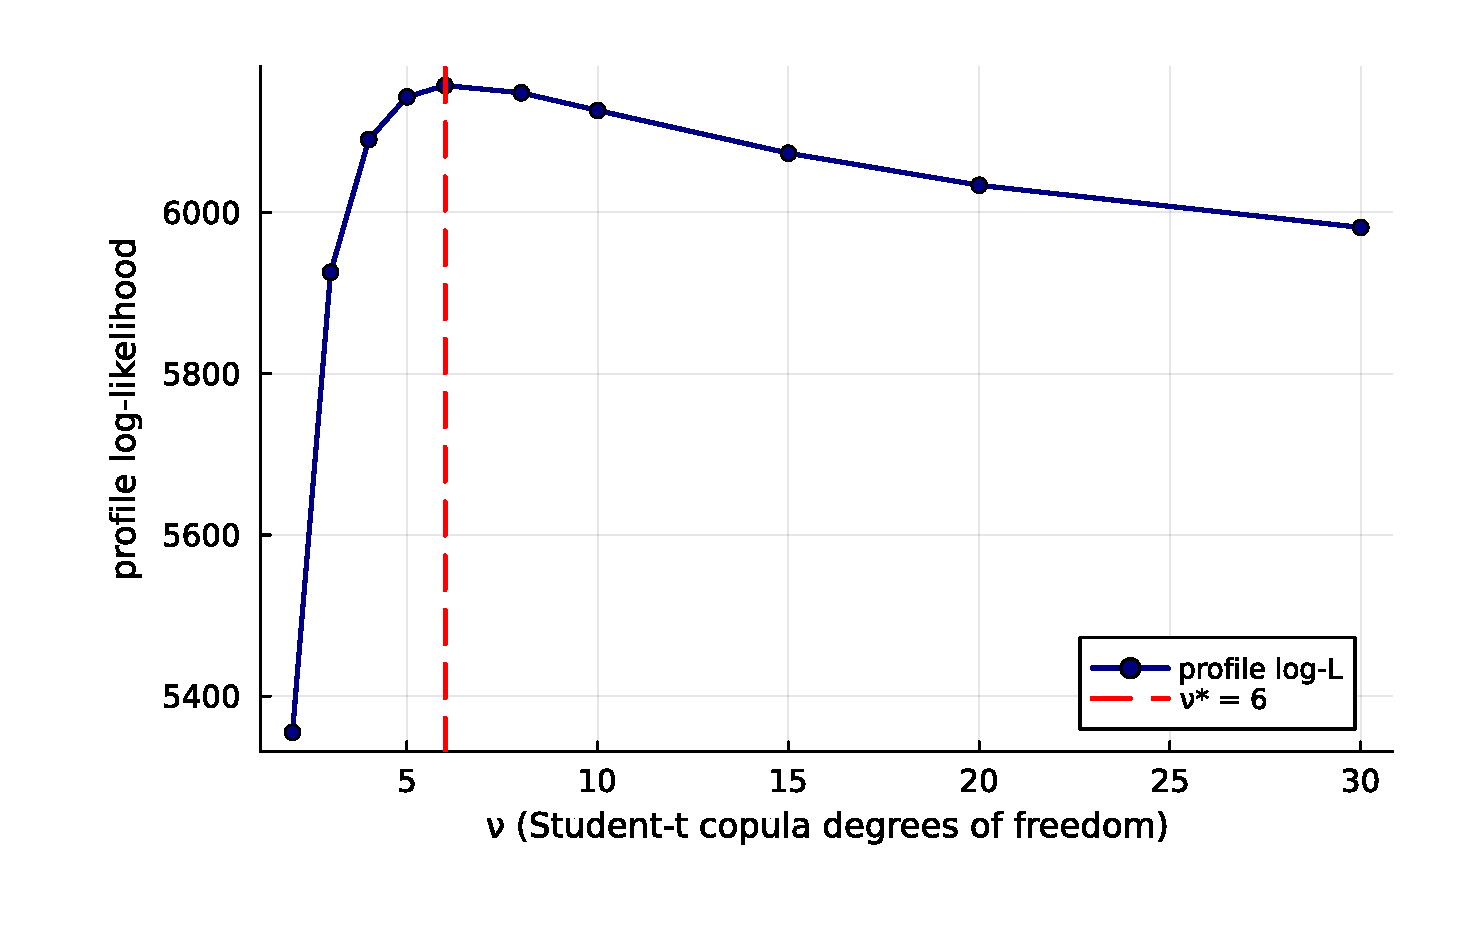
\includegraphics[width=0.70\textwidth]{figs/Fig-Copula-Profile.pdf}
\caption{\textbf{Profile log-likelihood of the Student-t copula} used inside Pipeline~B on the six-asset SPY cross-section (SPY, NVDA, JNJ, JPM, AAPL, QQQ; IS window 2014-01-03 through 2024-01-03). The vertical axis is the profile log-likelihood evaluated at each degrees-of-freedom value $\nu$ on the grid $\{2, 3, 4, 5, 6, 8, 10, 15, 20, 30\}$; the dashed red line marks the profile MLE $\nu^{*} = 6$ (peak value 6157.47). The CHMM-N marginals are held fixed at the Pipeline~A per-asset fits while $\nu$ is varied.}
\label{fig:copula_profile}
\end{figure}

\subsubsection{Cross-Asset Correlation Heat Maps (Pipeline~B, Companion to Table~\ref{tab:cross_asset_supp_summary})}
\label{sec:cross_asset_corr_supp}

Figure~\ref{fig:cross_asset_corr} visualises the observed and path-averaged simulated correlation matrices for the dependence models of Section~\ref{sec:cross_asset}.
The panel ordering is SIM, Gaussian copula, Student-t copula (each reported quantitatively in Table~\ref{tab:cross_asset_supp_summary}), plus a truncated C-vine variant with SPY as root for visual comparison.
All five panels share the six-asset SPY cross-section and the same CHMM-N marginals at $K = 18$, so any visible differences between the simulated panels reflect only the dependence construction.

\begin{figure}[H]
\centering
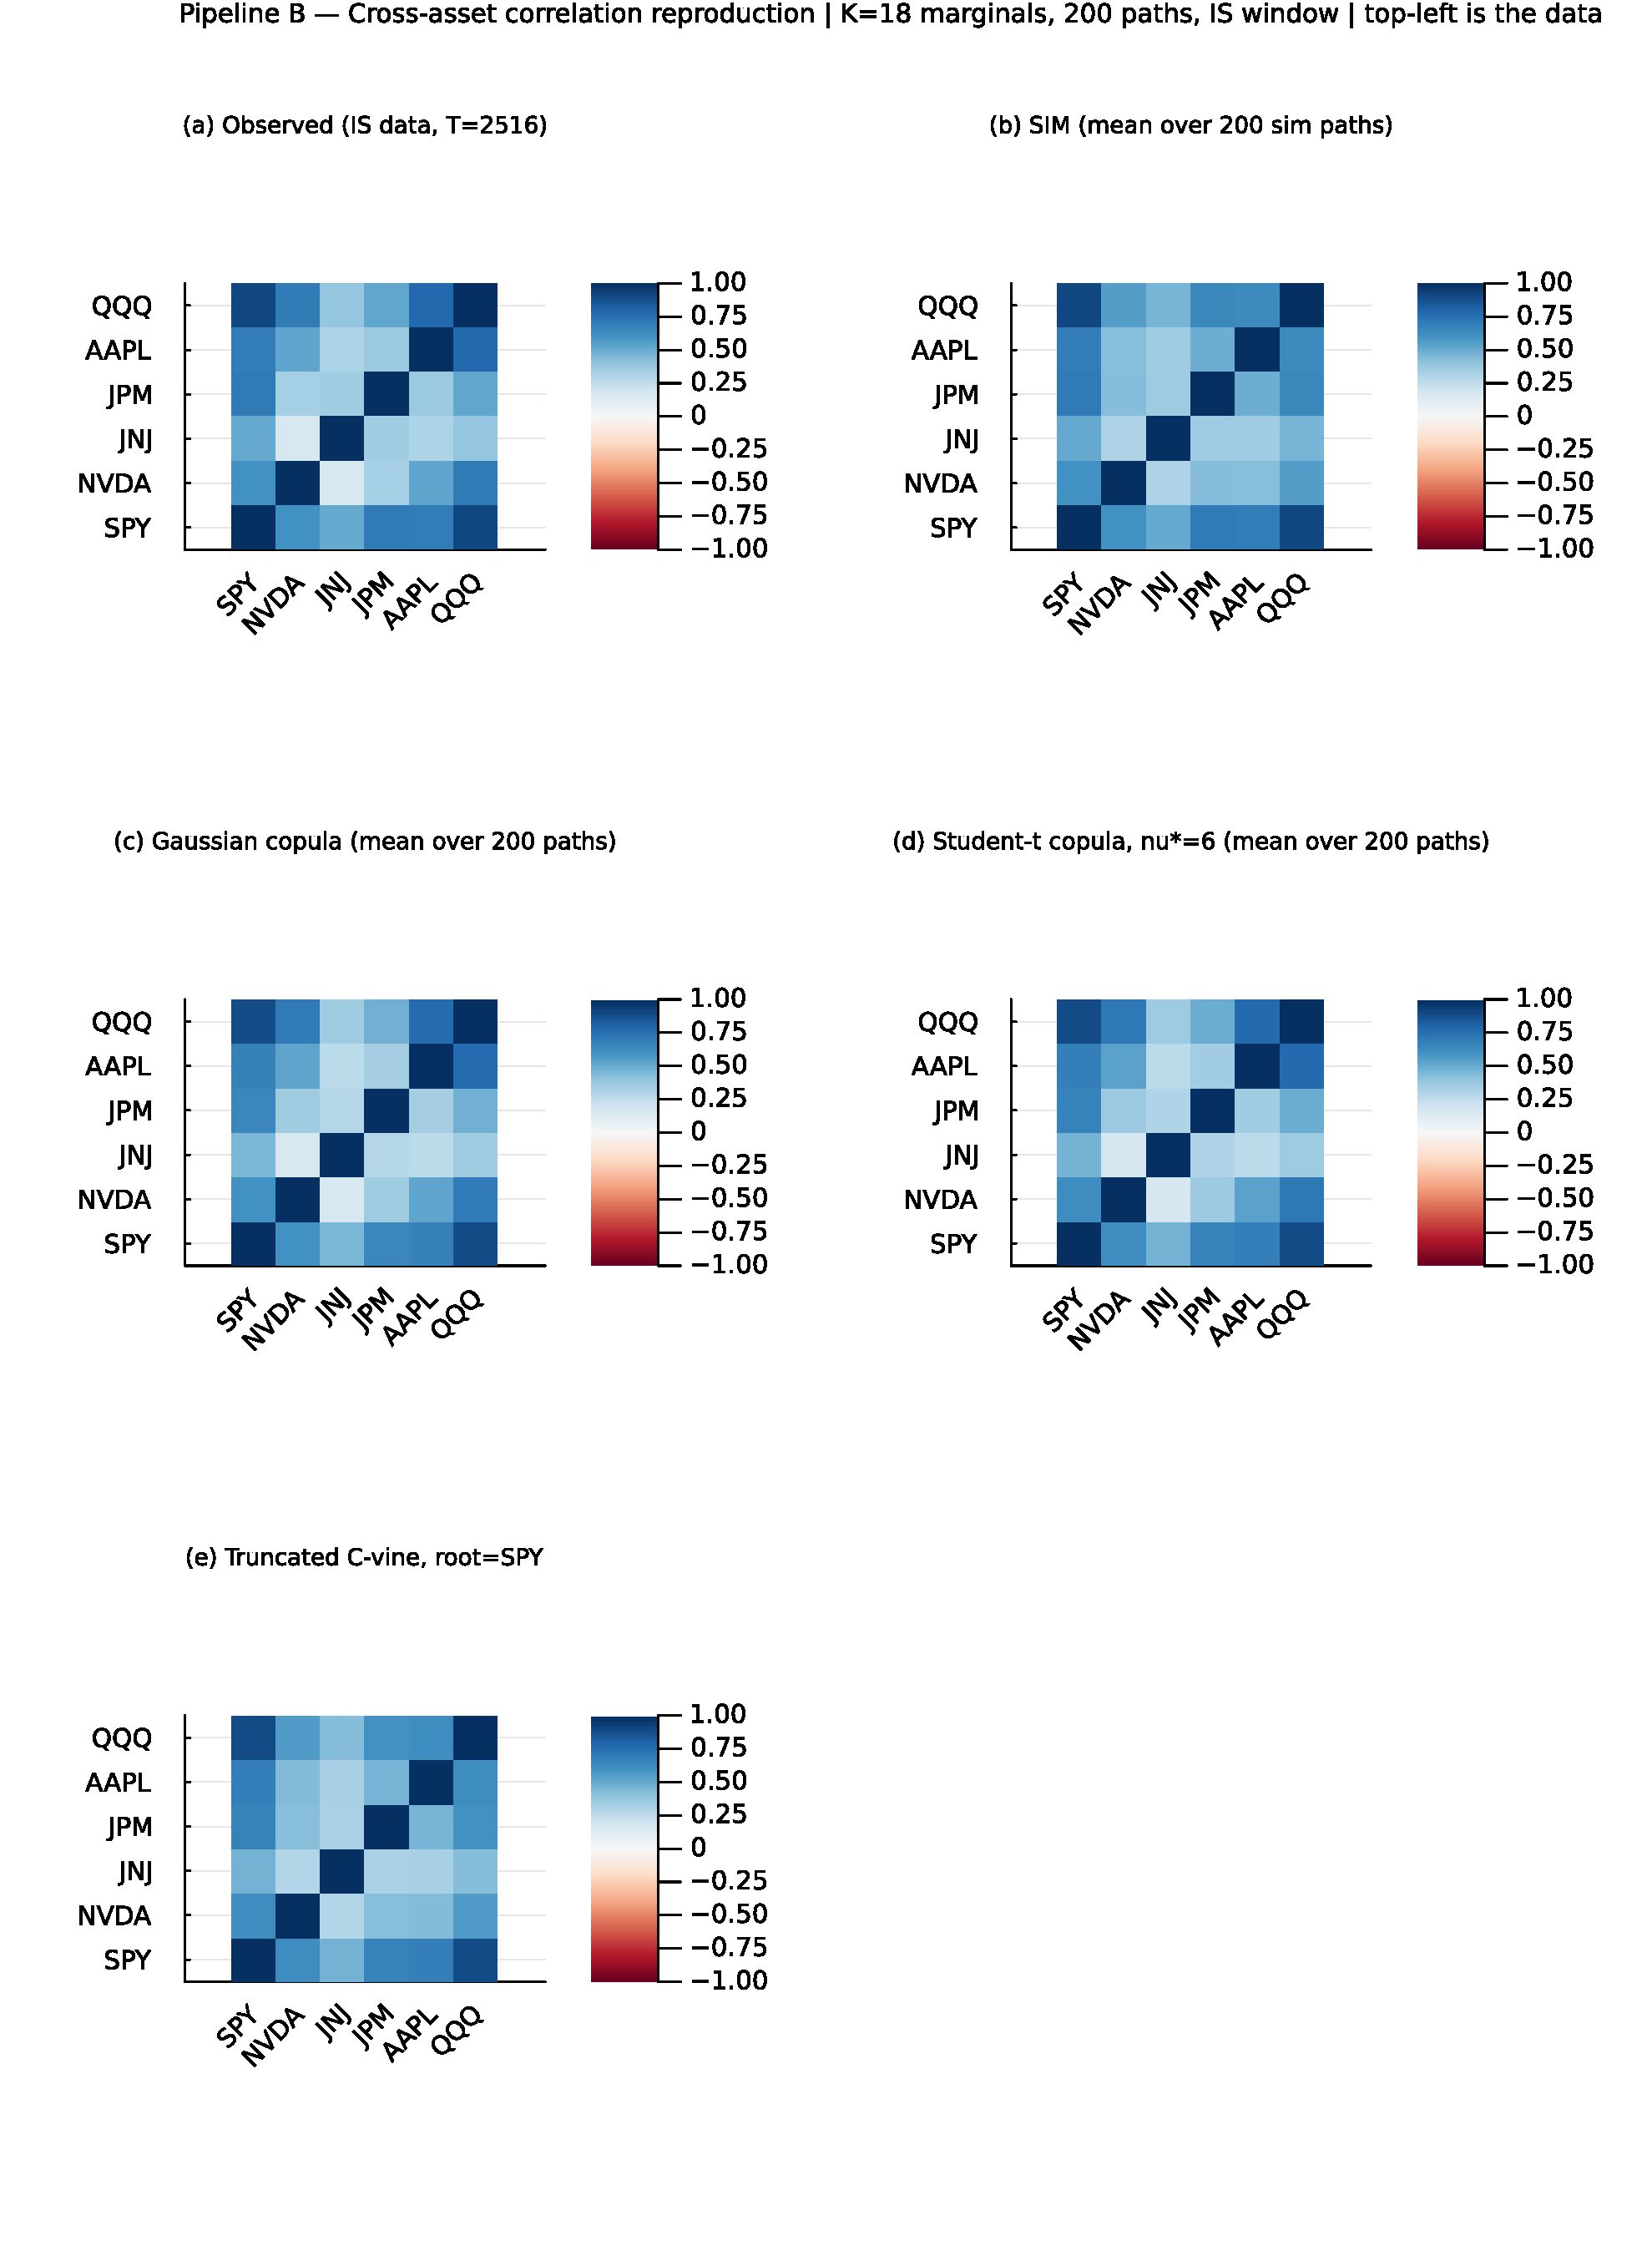
\includegraphics[width=0.75\textwidth]{figs/Fig-Cross-Asset-Correlation.pdf}
\caption{\textbf{Cross-asset IS correlation reproduction across dependence models} (Pipeline~B, companion to Table~\ref{tab:cross_asset_supp_summary}). Panel~(a), top-left: \emph{observed} correlation matrix on 2014-01-03 through 2024-01-03 daily excess log returns for SPY, NVDA, JNJ, JPM, AAPL, QQQ (IS window, $T_{\text{IS}} = 2{,}516$). Panel~(b), top-right: path-averaged correlation under the Single Index Model with SPY as market factor. Panel~(c), middle-left: path-averaged correlation under the Gaussian copula on CHMM marginals. Panel~(d), middle-right: path-averaged correlation under the Student-t copula on CHMM marginals, $\nu^* = 6$. Panel~(e), bottom-left: path-averaged correlation under a truncated C-vine copula with SPY as root. Each simulated panel averages over 200 paths of length $T_{\text{IS}}$. All marginals are the per-asset CHMM-N fits at $K = 18$ from Table~\ref{tab:cross_asset}; color scale in $[-1, 1]$, red-white-blue (RdBu) diverging. Closer visual match to panel~(a) is better.}
\label{fig:cross_asset_corr}
\end{figure}

\subsubsection{Non-US Asset Class Extension and Per-Pair OoS Off-Diagonal Breakdown}
\label{sec:non_us_asset_supp}

The body universe (SPY, NVDA, JNJ, JPM, AAPL, QQQ) is six US-listed equity tickers from one country-index family. To probe whether the cross-asset construction generalises off the equity cluster we extend the universe with GLD (SPDR Gold Trust), a US-listed ETF whose underlying is physically-backed gold, i.e.\ a non-equity commodity asset class.

\paragraph{GLD Pipeline-A univariate fidelity.}
Fitting CHMM-N, CHMM-t, and CHMM-L on the GLD return series at $K = 18$ produces $100\%$ IS KS pass rate for all three families and observed IS excess kurtosis $3.6$ matched closely by CHMM-L ($2.2$); on OoS, however, the KS pass rate collapses to $0\%$ for all three families against an observed OoS excess kurtosis of $6.5$. Inspection of the GLD price path on the $2024$--$2026$ OoS window shows the asset re-priced from $\sim 200$ to $\sim 300$ on a persistent demand shock not represented in the $2014$--$2024$ IS regime library. This is the same stationarity-scope artefact as the NVDA / JPM single-name OoS cliffs reported in Section~\ref{sec:cross_asset_univariate}, on a non-equity asset; the limitation is not equity-specific.

\paragraph{Pipeline-B: 7-ticker Student-t copula off-diagonal MAE.}
Refitting the Student-t copula on the augmented seven-ticker universe at $\nu^\star = 6$ gives IS off-diagonal MAE of $0.029$ (six-ticker baseline: $0.027$) and OoS off-diagonal MAE of $0.179$ (six-ticker baseline: $0.211$). Adding the low-equity-correlation gold ETF \emph{reduces} the OoS off-diagonal MAE, because the equity-cluster correlation degradation is the dominant component; pairs involving GLD have moderate IS-to-OoS shifts ($|\Delta| \in [0.04, 0.19]$) while the largest equity-cluster pairs (JNJ-QQQ, SPY-JNJ, NVDA-JNJ) have $|\Delta| > 0.48$ on OoS.

\paragraph{Per-pair OoS gap localisation.}
Table~\ref{tab:per_pair_offdiag_mae} reports the per-pair off-diagonal absolute deviation between observed and path-averaged simulated correlation matrices on IS and OoS, sorted by OoS $|\Delta|$. The OoS gap concentrates in pairs involving JNJ (the defensive single-name proxy): JNJ's IS correlation with the broad equity factor (QQQ, SPY) collapses on OoS, in some pairs flipping sign, and the IS-fixed copula has no mechanism for tracking that shift. The gold-ETF pairs (SPY-GLD, JPM-GLD, JNJ-GLD, QQQ-GLD) sit in the middle of the ranking with $|\Delta|$ between $0.10$ and $0.19$ on OoS. The dominant cause of the OoS off-diagonal gap is therefore neither equity-cluster size nor copula-degree mis-specification but a single-name regime shift in the JNJ-equity-factor relationship that the IS-fitted dependence layer cannot anticipate.

\begin{table}[t]
\centering
\small
\caption{\textbf{Per-pair off-diagonal correlation MAE on the seven-ticker universe} (Pipeline B, Student-t copula on CHMM-N marginals at $K = 18$, $200$ paths, $\nu^\star = 6$). For each ticker pair $(i, j)$ the table reports $|\Sigma_{\text{sim,avg}}[i,j] - \Sigma_{\text{obs}}[i,j]|$ on IS and OoS, ranked by OoS $|\Delta|$. Only the ten largest-OoS-gap pairs are shown for compactness.}
\label{tab:per_pair_offdiag_mae}
\begin{tabular}{l c c c}
\toprule
Pair & IS $|\Delta|$ & OoS $|\Delta|$ & OoS $-$ IS \\
\midrule
JNJ-QQQ   & $0.027$ & $0.544$ & $0.517$ \\
SPY-JNJ   & $0.037$ & $0.509$ & $0.473$ \\
NVDA-JNJ  & $0.017$ & $0.489$ & $0.473$ \\
NVDA-AAPL & $0.011$ & $0.278$ & $0.268$ \\
JNJ-JPM   & $0.046$ & $0.261$ & $0.216$ \\
JNJ-AAPL  & $0.042$ & $0.244$ & $0.202$ \\
AAPL-QQQ  & $0.003$ & $0.227$ & $0.224$ \\
JPM-GLD   & $0.027$ & $0.187$ & $0.160$ \\
SPY-GLD   & $0.038$ & $0.127$ & $0.089$ \\
JNJ-GLD   & $0.015$ & $0.117$ & $0.101$ \\
\bottomrule
\end{tabular}
\end{table}




\subsection{\texorpdfstring{Pre-OoS Validation $K$-Selection, Walk-Forward Summary, and $\nu_k$ Diagnostics}{Pre-OoS Validation K-Selection, Walk-Forward Summary, and nu\_k Diagnostics}}
\label{sec:supp_misc}

\paragraph{Pre-OoS validation $K$-selection.}
The $K = 18$ operating point in the main panel was chosen via a multi-objective criterion combining information-criterion (IC) rank with IS and OoS distributional pass rates, which uses the same $2024$--$2026$ window later used for VaR. As a clean re-selection that decouples the two, we fit CHMM-N on $2014$-$01$-$03$ through $2021$-$12$-$31$ ($n = 2{,}013$) and score every $K$ in the sweep by the forward-algorithm held-out log-likelihood on $2022$-$01$-$03$ through $2024$-$01$-$03$ ($n = 502$); the $2024$--$2026$ window is not touched. Held-out log-lik, BIC, HQC, and CAIC all select $K^\star = 3$ (per-observation log-lik $-2.5345$ at $K = 3$ vs.\ $-2.5694$ at $K = 18$); AIC selects $K^\star = 6$; held-out two-sample KS selects $K^\star = 9$. None of the six criteria that avoid the OoS window select $K = 18$. The $K = 18$ choice is best read as a multi-metric one that weights tail fidelity (kurtosis, AD) and downstream VaR behaviour alongside likelihood; a parallel main panel at $K = 3$ would re-rank some rows in CHMM's favour on ACF-MAE and against it on tail fidelity. The $2022$--$2023$ validation slice is itself partly a structural-break period (the rate-hike cycle), so any model with substantial IS-specific structure generalises worse on it.

\paragraph{$\nu_k$ bracket and penalised-ECM rate sweep.}
A bracket sweep $\nu_{\min} \in \{2.1, 2.5, 3.0, 4.0\}$ shows the CHMM-t fit does not pile against the lower bracket: median $\nu_k = 50$, only $2/18$ states near the lower edge. Lifting $\nu_{\min}$ does not reduce the $14.30 \to 7.69$ overshoot because the fit shifts posterior mass into the newly-recentred tail states. An exponential $1/\nu_k$ shrinkage prior at rate $\lambda \in \{0, 5, 20, 50, 100, 200\}$ reduces simulated excess kurtosis monotonically: $14.30, 11.19, 8.43, 5.41, 3.96, 3.67$. The recommended rate $\lambda = 20$ brings simulated kurtosis to $\approx 8$ (close to the observed $7.69$) at a $1$pp IS KS cost. Only the $\nu_{\min}$ state parameter actually moves ($2.1 \to 4.89$); upper bracket and median remain at $50$. The overshoot is therefore a single-state artefact of the two tail regimes hitting the lower bracket under unpenalised ECM.

\paragraph{Cross-asset summary.}
The full per-construction Pipeline~B panel is in Section~\ref{sec:supp_cross_asset}; for reference, the headline ordering is summarised in Table~\ref{tab:cross_asset_supp_summary}.

\begin{table}[h]
\centering
\small
\caption{\textbf{Cross-asset dependence summary} (Pipeline~B; CHMM-N marginals at $K = 18$; $200$ paths). Median per-asset KS pass rate (\%) and off-diagonal MAE of the simulated correlation matrix vs.\ observed. The Student-t copula at $\nu^\star = 6$ is the strongest dependence layer on every IS metric; full per-asset detail is in Section~\ref{sec:supp_cross_asset}.}
\label{tab:cross_asset_supp_summary}
\begin{tabular}{l c c c c}
\toprule
& Median IS KS & Median OoS KS & Off-diag MAE IS & Off-diag MAE OoS \\
\midrule
Single Index Model       & $78.5$  & $85.0$  & $0.076$ & $0.261$ \\
Gaussian copula          & $97.8$  & $87.2$  & $0.031$ & $0.202$ \\
Student-t copula ($\nu^\star = 6$) & $\mathbf{96.0}$  & $\mathbf{89.8}$  & $\mathbf{0.027}$ & $\mathbf{0.208}$ \\
\bottomrule
\end{tabular}
\end{table}
